\documentclass[conference]{IEEEtran}
\IEEEoverridecommandlockouts
% The preceding line is only needed to identify funding in the first footnote. If that is unneeded, please comment it out.
\usepackage{amsmath,amssymb,amsfonts}
\usepackage{algorithmic}
\usepackage{graphicx}
\usepackage[inline, shortlabels]{enumitem}
\usepackage{tabularx}
\usepackage{caption}
\usepackage{titlesec}
\usepackage[T2A,T1]{fontenc}
\usepackage[english]{babel}
\captionsetup{font=it}
\usepackage{ragged2e}
\usepackage{hyperref}
\usepackage{pifont}
\usepackage{footmisc}
\usepackage{multirow}

% --- Tickz
\usepackage{physics}
\usepackage{amsmath}
\usepackage{tikz}
\usepackage{mathdots}
\usepackage{yhmath}
\usepackage{cancel}
\usepackage{color}
\usepackage{siunitx}
\usepackage{array}
\usepackage{multirow}
\usepackage{amssymb}
\usepackage{gensymb}
\usepackage{tabularx}
\usepackage{extarrows}
\usepackage{booktabs}
\usetikzlibrary{fadings}
\usetikzlibrary{patterns}
\usetikzlibrary{shadows.blur}
\usetikzlibrary{shapes}
% ---------

\usepackage{pdfpages}
\usepackage{booktabs}
\usepackage{csquotes}
\usepackage{lipsum}  
\usepackage{arydshln}
\usepackage{smartdiagram}
\usepackage[inkscapeformat=png]{svg}
\usepackage{textcomp}
\usepackage{tabularray}\UseTblrLibrary{varwidth}
\usepackage{xcolor}
\def\BibTeX{{\rm B\kern-.05em{\sc i\kern-.025em b}\kern-.08em
    T\kern-.1667em\lower.7ex\hbox{E}\kern-.125emX}}
\usepackage{cite}
\usepackage{amsmath}
\newcommand{\probP}{\text{I\kern-0.15em P}}
\usepackage{etoolbox}
\patchcmd{\thebibliography}{\section*{\refname}}{}{}{}

\setlength{\extrarowheight}{2.5pt}

% \renewcommand{\arraystretch}{1.7}

% \setlength{\extrarowheight}{2.5pt}
% \renewcommand{\arraystretch}{0.2}
% \renewcommand{\arraystretch}{1.7}

% --------------
\titleclass{\subsubsubsection}{straight}[\subsection]

\newcounter{subsubsubsection}[subsubsection]
\renewcommand\thesubsubsubsection{\thesubsubsection.\arabic{subsubsubsection}}
\renewcommand\theparagraph{\thesubsubsubsection.\arabic{paragraph}} % optional; useful if paragraphs are to be numbered

\titleformat{\subsubsubsection}
  {\normalfont\normalsize\bfseries}{\thesubsubsubsection}{1em}{}
\titlespacing*{\subsubsubsection}
{0pt}{3.25ex plus 1ex minus .2ex}{1.5ex plus .2ex}

\makeatletter
\renewcommand\paragraph{\@startsection{paragraph}{5}{\z@}%
  {3.25ex \@plus1ex \@minus.2ex}%
  {-1em}%
  {\normalfont\normalsize\bfseries}}
\renewcommand\subparagraph{\@startsection{subparagraph}{6}{\parindent}%
  {3.25ex \@plus1ex \@minus .2ex}%
  {-1em}%
  {\normalfont\normalsize\bfseries}}
\def\toclevel@subsubsubsection{4}
\def\toclevel@paragraph{5}
\def\toclevel@paragraph{6}
\def\l@subsubsubsection{\@dottedtocline{4}{7em}{4em}}
\def\l@paragraph{\@dottedtocline{5}{10em}{5em}}
\def\l@subparagraph{\@dottedtocline{6}{14em}{6em}}
\makeatother

\setcounter{secnumdepth}{4}
\setcounter{tocdepth}{4}
% --------------


\newcommand{\before}[1]{\textcolor{red}{#1}}
\newcommand{\after}[1]{\textcolor{green}{#1}}

\newcommand{\old}[1]{\textcolor{orange}{#1}}
\newcommand{\rem}[1]{\textcolor{red}{#1}}
\newcommand{\todo}[1]{\textcolor{orange}{\newline \textit{\textbf{TODO:} #1}} \newline \newline }

\makeatletter
\newcommand{\linebreakand}{%
  \end{@IEEEauthorhalign}
  \hfill\mbox{}\par
  \mbox{}\hfill\begin{@IEEEauthorhalign}
}
\makeatother




% ---------------------------


\begin{document}

\title{CybMASFM: A Formal Model for Cyberdefense Multi-Agent Systems\\
    % {\footnotesize \textsuperscript{Note}}
    % \thanks{Identify applicable funding agency here. If none, delete this.}
}

% \IEEEaftertitletext{\vspace{-1\baselineskip}}

\author{

    \IEEEauthorblockN{Julien Soulé}
    \IEEEauthorblockA{\textit{Thales Land and Air Systems, BU IAS}}
    %Rennes, France \\
    \IEEEauthorblockA{\textit{Univ. Grenoble Alpes,} \\
        \textit{Grenoble INP, LCIS, 26000,}\\
        Valence, France \\
        julien.soule@lcis.grenoble-inp.fr}

    \and

    \IEEEauthorblockN{Jean-Paul Jamont\IEEEauthorrefmark{1}, Michel Occello\IEEEauthorrefmark{2}}
    \IEEEauthorblockA{\textit{Univ. Grenoble Alpes,} \\
        \textit{Grenoble INP, LCIS, 26000,}\\
        Valence, France \\
        \{\IEEEauthorrefmark{1}jean-paul.jamont,\IEEEauthorrefmark{2}michel.occello\}@lcis.grenoble-inp.fr
    }

    % \and

    % \IEEEauthorblockN{Michel Occello}
    % \IEEEauthorblockA{\textit{Univ. Grenoble Alpes,} \\
    % \textit{Grenoble INP, LCIS, 26000,}\\
    % Valence, France \\
    % michel.occello@lcis.grenoble-inp.fr}

    \and

    \IEEEauthorblockN{Paul Théron}
    \IEEEauthorblockA{
        \textit{Co-leader of the IST-152 OTAN, 1st president of the AICA IWG} \\
        La Guillermie, France \\
        %lieu-dit Le Bourg, France \\
        paul.theron@orange.fr}

    % \linebreakand

    \and

    \IEEEauthorblockN{Louis-Marie Traonouez}
    \IEEEauthorblockA{\textit{Thales Land and Air Systems, BU IAS} \\
        Rennes, France \\
        louis-marie.traonouez@thalesgroup.com}}


\maketitle

% todo: "promising" -> trop fort
% before trying... -> implique une étape intermediaire alors qu'il s'agit d'un travail sur un modèle utilisable à plusieurs étapes

\begin{abstract}

    Collaboration among cyber-defender agents in a networked host system is a promising approach to tackle cyber-attacks as close as entry points. Indeed, cyber-defense agents that are making up a cyber-defense Multi-Agent System with a flexible organization could handle scalability and adaptivity issues relying on self/re-organization mechanisms. Yet, before empirically trying to implement it, we aim to frame the problem of organization as the design of cyber-defense agents that have to collaborate to reach a cyber-defense goal under the deployment environment constraints; and the means to solve that problem as organizational mechanisms such as multi-agent paradigms or multi-agent deep learning algorithms.
    The paper deals with a general formal model that aims to help framing the design of a cyber-defense multi-agent system by positioning it in related works of cyber-defense, multi-agent systems and reinforcement learning domains.

\end{abstract}

\begin{IEEEkeywords}
    cyberdefense, multi-agent systems, reinforcement learning, organization, formal
\end{IEEEkeywords}

\section{Introduction}

As stated within \textquote{Autonomous Intelligent cyber-defense Agents} works\cite{kott2023autonomous}, the increasing complexity of cyber-threats and the limitations of centralized cyber-defense systems have led to fostering a multi-agent approach of cyber-defense. In this approach, the cyber-defender agents are making up a cyber-defense Multi-Agent System (CMAS). We think this Multi-Agent System (MAS) can only be envisioned in a scenario as blue team that aims to achieve cyber-defense goals to fight against a red team of cyber-attacker agents and tackle their impact on the networked environment and regular users represented as a green team.

Consequently, the design of a CMAS should be made considering a scenario to be ultimately implemented. Yet, a direct empiric implementation of a scenario to assess various CMAS types, may skip important prior theoretical considerations as for the specific problem to be set up in the scenario and the theoretical means to address and solve it. Indeed, not only do we need to realistically and consistently describe and design the networked host environment, the blue, red and green teams; but we also need to theoretically apprehend the scenario when teams are operating ultimately giving means to apprehend and generalize the role of CMAS organization on various scenarios.

In a MAS, we refer to organization among agents as the set of their respective individual behavior whose the collective action impacts the distance expressing how far agents are from their common goal for anytime. We assume research in CMAS is mainly focusing on finding an organization that allows agents being the closest as possible to their common cyber-defense goal at given points.

% A theoretical scenario refers to a set of abstract descriptions or models defining at least partially each component of a scenario. Moreover, we assume a theoretical scenario can always be mapped to real scenarios where the components are real software or hardware assets relying on available hardware and software technology. We refer to development as the whole process allowing real scenarios to be obtained from a theoretical scenario. Therefore, research in CMAS requires developing theoretical scenarios to get some feedback of various organizations among cyber-defender agents.

Currently, we did not identify any directly usable work as for comprehensively modeling such a scenario as it requires considering both a Multi-Agent Systems (MAS) designing point-of-view for agents teams and a cyber-defense point-of-view for the networked environment, attacks and countermeasures.
Gaps between these two point-of-views shows the development of a CMAS lacks of consistent central models to design scenarios, implement and monitor them in simulation or emulation, and analyze results as their organizations.

Our main contribution is the Cyberdefense Multi-Agent Systems Formal Model (CybMASFM) comprising both a formal view of CMAS in a scenario to be used to build realistic models for later implementation, and theoretical means to apprehend its interactions and the key role of organization in various operating CMAS.

\begin{table*}[ht!]

    \centering

    \begin{tblr}{colspec={Q[l,m]Q[c,m]Q[c,m]Q[c,m]Q[c,m]Q[c,m]Q[c,m]Q[c,m]Q[c,m]Q[c,m]Q[c,m]Q[c,m]Q[c,m]Q[c,m]Q[c,m]Q[c,m]},rows={m},measure=vbox,stretch=-1}

        {} & \textbf{\cite{thompson2018}} & \textbf{\cite{aydin2023}} & \textbf{\cite{kotenko2007}} & \textbf{\cite{elhachem2018}} & \textbf{\cite{dan2021}} & \textbf{\cite{Seo2022-ai}} & \textbf{\cite{gulosh2018employment}} & \textbf{\cite{kott2018autonomous}} & \textbf{\cite{padgett2017defensive}} & \textbf{\cite{skroch2009modeling}} & \textbf{\cite{ hamilton2008}} & \textbf{\cite{kavak2021}} & \textbf{\cite{yohanandhan2020cyber}} & \textbf{\cite{attiah2018game}} & \textbf{\cite{leblanc2011overview}} \\
        %& \textbf{\cite{rajivan2013agent}} & \textbf{\cite{nguyen2021deep}} & \textbf{\cite{bergin2015cyber}} & \textbf{\cite{chi2001network}} \\

        \hline

        \\

        { Formal } & { \checkmark } & {  } & {  } & {  } & {  } & { \checkmark } & {  } & {  } & { \checkmark } & { \checkmark } & {  } & {  } & {  } & {  } & {  } \\
        
        { General } & {  } & { \checkmark } & {  } & {  } & {  } & {  } & {  } & {  } & {  } & { \checkmark } & { \checkmark } & {  } & {  } & {  } & {  } \\

        { Designed for implementation } & { \checkmark } & { \checkmark } & {  } & { \checkmark } & {  } & {  } & { \checkmark } & {  } & {  } & { \checkmark } & {  } & {  } & { \checkmark } & {  } & {  } \\

        { Designed for Green team } & {  } & {  } & {  } & {  } & {  } & { \checkmark } & {  } & {  } & {  } & {  } & {  } & {  } & {  } & { \checkmark } & {  } \\

        { Designed for Red team } & { \checkmark } & {  } & { \checkmark } & { \checkmark } & { \checkmark } & { \checkmark } & { \checkmark } & { \checkmark } & { \checkmark } & {  } & { \checkmark } & {  } & { \checkmark } & {  } & {  } \\

        { Designed for Blue team } & {  } & {  } & { \checkmark } & { \checkmark } & {  } & {  } & { \checkmark } & { \checkmark } & {  } & {  } & {  } & { \checkmark } & {  } & {  } & { \checkmark } \\

        { Fidel to reality } & {  } & {  } & {  } & {  } & {  } & {  } & { \checkmark } & {  } & {  } & { \checkmark } & {  } & { \checkmark } & { \checkmark } & {  } & {  } \\

        { Used for experiments } & {  } & {  } & {  } & {  } & {  } & {  } & {  } & {  } & {  } & {  } & {  } & {  } & { \checkmark } & {  } & {  } \\

        { Designed for organization analysis } & {  } & {  } & {  } & {  } & {  } & {  } & { \checkmark } & {  } & {  } & {  } & {  } & {  } & {  } & {  } & {  } \\

        { Designed for MARL } & {  } & {  } & {  } & { \checkmark } & {  } & {  } & { } & {  } & {  } & { } & {  } & {  } & { } & { \checkmark } & { \checkmark } \\

    \end{tblr}

    \caption{An analysis of selected related works covering criteria for a scenario model}

    \label{tab:cmas_formal_model_review}
    
\end{table*}


In section II, we first exposed an informal overview of our vision of an operating CMAS showing how related works in cyber-defense, multi-agent and machine learning domains are thought to be key means to envision scenarios.
In section III, we introduced the fundamentals of the CybMASFM as an integrative formal model to describe a scenario so that a CMAS can be positioned within a same design space; also enabling thorough analysis and comparison between various CMAS types on scenarios.
In section IV, we detailed how CybMASFM integrates cyber-defense and cyber-attack frameworks, Multi-Agent Reinforcement Learning (MARL) algorithms and MAS mechanisms to design blue, green and red teams actions, observations, behavior and rewards.
In section V, we proposed a new approach to envision organization combining classical MAS mechanisms with MARL to unify bottom-up and top-down design approaches showing any point-of-view ranging between these two extrema can be envisioned in CybMASFM.
In section VI, we proposed using CybMASFM to model drone swarm scenarios coming from the third CAGE Challenge\cite{cage_challenge_3_announcement}. We characterized the scenario models as for deployment environment, blue and red teams objectives and organizations for ten of the proposed solutions. We showed CybMASFM can be used to consistently analyze relations between environment, objectives and organization of a CMAS.
In section VII, we concluded on the viability of CybMASFM also showing identified limitations we aim to overcome as perspectives for a wider utility.


\section{Related works}

We identified works that partially rely on modeling the scenario of a CMAS considering both a MAS designing point-of-view for agent teams and a cyber-defense point-of-view for the networked environment, attacks, and countermeasures. Formally, we first conducted a research of works according to the following boolean keywords: ("cyber-attack" or "cyber-defense") or "model" or "simulation" or "agent". Selected works implying a model dealing with the equivalent of red, blue or green in a networked system, were further analyzed with respect to 10 criteria onto the model:

\begin{itemize}
    \item Formal: Is the model relying on any formalism?
    \item General: Is the model applicable in generic scenarios?
    \item Designed for implementation: Is the model a medium to be used during implementation?
    \item Designed for Green Team: Does the model integrate the regular users?
    \item Designed for Blue Team: Does the model integrate the cyberdefense?
    \item Designed for Red Team: Does the model integrate the cyber-attacks
    \item Fidel to reality: Is the model close to real cyber-attack, countermeasures
    \item Used for experiments: Have experiments used the model as a medium?
    \item Designed for organization analysis: Does the model provide means to analyze and design organization in for the blue team?
    \item Designed for MARL: Is the model usable to apply RL algorithms for red and blue teams?
\end{itemize}

Only 16 considered works cover more than one the criteria. Results are summarized in Table \ref{tab:cmas_formal_model_review}.

From results, we observed most of available works do not meet all of the criteria especially as for having both a model to be used in implementation and in a general way. Moreover, almost none of the selected works cover the need to analyze the organization among agents. In a more general way, we consider 4 categories of works: the specific applicative models, the simulation models, the emulation models, the general frameworks. Here we present some representative works for each category.

% "Defensive Swarm: An Agent Based Modeling Analysis" deals with an agent-based computer simulation model for tactical problem of defending against enemies' attacks. It takes into account interaction between defenders and enemies\cite{padgett2017defensive}.

% "Autonomous Intelligent Cyber-defense Agent (AICA) Reference Architecture, Release 2.0" deals with architecture model for Intelligent software agents performing active, largely autonomous cyber-defense actions on military networks\cite{kott2018autonomous}.

% "Employment of Intelligence, Surveillance, and Reconnaissance Drone swarms to enhance ground combat operations" deals with modeling and simulation of drone swarm architecture in a combat scenario\cite{gulosh2018employment}.

% "D-CEWS: DEVS-Based Cyber-Electronic Warfare M\&S Framework for Enhanced Communication Effectiveness Analysis in Battlefield" deals with wargame models using agent-based modeling. It takes into account actor's attack and defense state components within the cyber-electronic warfare-based battlefield scenario\cite{Seo2022-ai}.

% "Multi-agent Modelling and Simulation of Cyber-Attacks and Cyber-Defense for Homeland Security" - This work presents an approach based on the agent-based simulation of cyber-attacks and cyber-protection mechanisms, combining discrete-event simulation, multi-agent modeling, and simulation for homeland security\cite{kotenko2007}.

"Internet of things security: A multi-agent-based defense system design" - The literature review in this work focuses on agent-based approaches in cyber defense and presents a multi-agent-based defense system design for the security of the Internet of Things, considering cyber-attacks and defense mechanisms\cite{aydin2023}.

"Extending a Multi-Agent Systems Simulation Architecture for Systems-of-Systems Security Analysis" - This document presents an approach for extending a multi-agent systems simulation architecture for systems-of-systems security analysis, including the manual derivation of risks and use case descriptions, which is relevant for cyber-defense scenario modeling\cite{elhachem2018}.

"An agent-based modeling framework for cybersecurity in mobile tactical networks" - This framework focuses on agent-based simulation as a modeling methodology for analyzing the effects of individuals' actions and interactions on a dynamic system, specifically in the context of cybersecurity in mobile tactical networks, which can be applied to the design and assessment of CMAS in various scenarios\cite{thompson2018}.

"Physical Safety and Cyber Security Analysis of Multi-Agent Systems: A Survey of Recent Advances" - This survey provides an overview of recent advances in the analysis of multi-agent systems, including their application to cyber security, which can offer valuable insights for the theoretical and practical considerations of modeling CMAS for cyber-defense scenarios\cite{dan2021}.


\section{Fundamentals for a CMAS formal model}

The idea of a CMAS involves considering both the vision of MASs and their development and the world of cyber-defense in particular its constraints. However, reconciling these two areas leads to considering a priori two opposing points of view.

From the point of view of MAS towards Cyberdefense, the process of developing a CMAS could be envisaged as the extension of the multi-agent paradigm to Cyberdefense which would only be one area of application. This process would firstly be based on approaches, methods or models from the world of MASs which would need to be highlighted and adapted to respond to identified constraints and needs arising from Cyberdefense. For example, organizational paradigms applied to cyber-defense agents such as hierarchies, models based on markets, teams could be considered in this approach. The application of these organizational paradigms could make it possible to meet needs such as scaling up when increasing load, reactivity in detecting and responding to attacks, execution performance during implementation of countermeasures, etc.

From the point of view of Cyberdefense towards MASs, the process of developing a CMAS could be envisaged as taking advantage of capabilities from the multi-agent paradigm to increase the capabilities of Cyberdefense systems with the timely aim of face specific challenges and constraints. This process would emphasize the identification of the needs and constraints of the systems to be protected, which could be shown to be covered by the application of certain tailor-made multi-agent mechanisms. For example, in a cyber-defense system protecting an open network system, the problem of adapting the cyber-defense system to changes in network topology could be covered by the redundant deployment of autonomous protection agents as part of the cyber-defense system.

The approach of our vision in the development of a CMAS considers these two points of view in a complementary manner. First, the development of a CMAS could benefit from feedback from first attempts at creation and experimentation with an MAS approach to cyber-defense in order to understand the impact of multi-agent mechanisms to cover constraints and needs identified on several case studies. In doing so, it would contribute to enriching the known links between Cyberdefense constraints and multi-agent mechanisms for the Cyberdefense point of view towards MASs. The accumulated experiences and knowledge could allow the application of the cyber-defense point of view to MAS by directly advocating the multi-agent mechanisms to be considered to precisely cover the identified cyber-defense constraints and needs.

Our vision of development uses several approaches, terms, concepts and notions that it is necessary to formalize and rationalize in order to have a common and coherent framework in which it would make sense to rigorously present our vision of the development of an MAS of Cyberdefense. No current work is intentionally part of this approach to building a link between the multi-agent paradigm and cyber-defense. For this reason, we propose CybMASFM as a basic structure to understand and rigorously organize the concepts related to our vision of a CMAS and its development.

\begin{figure*}[]
    \centering
    


\tikzset{every picture/.style={line width=0.75pt}} %set default line width to 0.75pt        

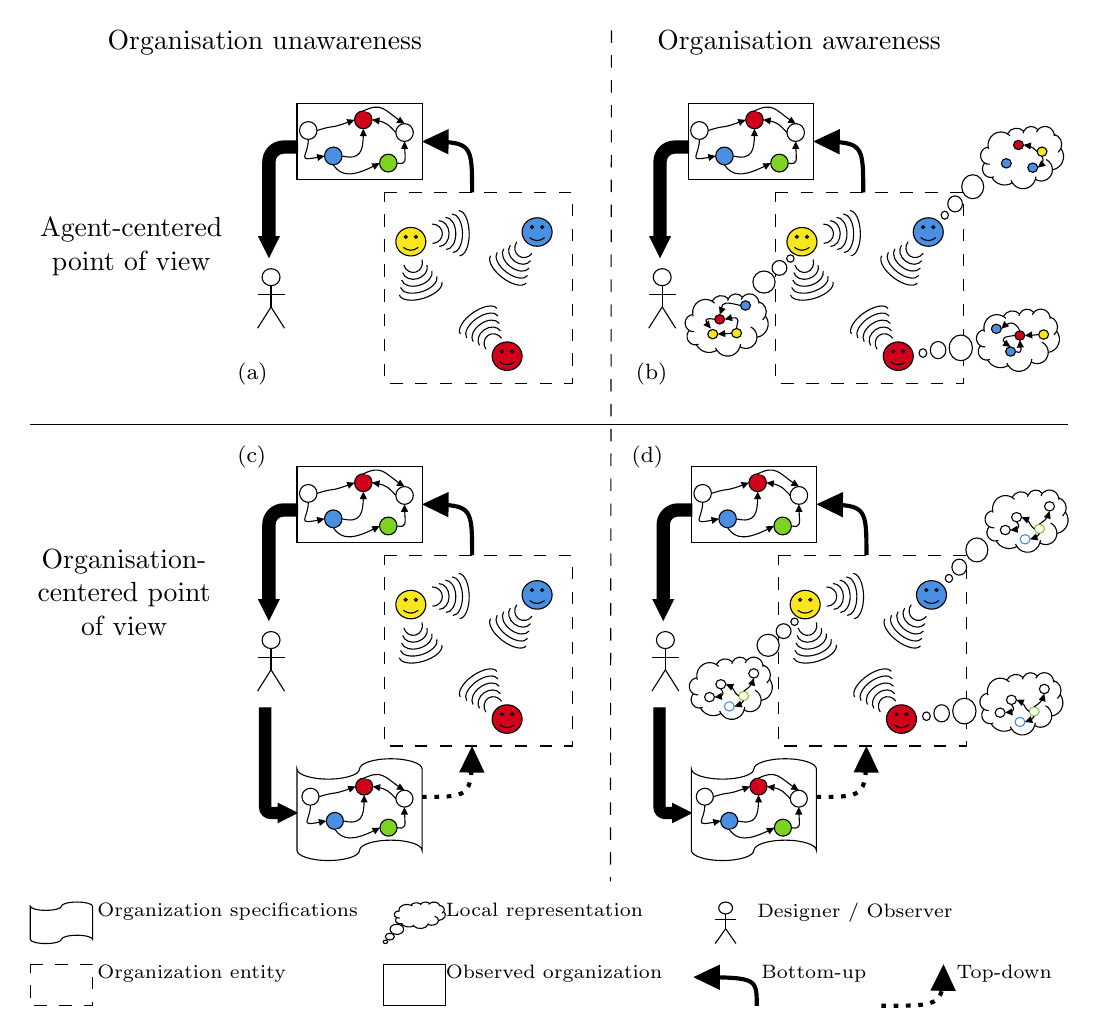
\begin{tikzpicture}[x=0.75pt,y=0.75pt,yscale=-1,xscale=1]
%uncomment if require: \path (0,558); %set diagram left start at 0, and has height of 558

%Shape: Cloud [id:dp19528938797470152] 
\draw  [fill={rgb, 255:red, 255; green, 255; blue, 255 }  ,fill opacity=1 ] (331.14,331.88) .. controls (330.82,329.46) and (331.88,327.06) .. (333.86,325.71) .. controls (335.85,324.36) and (338.42,324.28) .. (340.48,325.51) .. controls (341.21,324.11) and (342.55,323.14) .. (344.09,322.89) .. controls (345.63,322.65) and (347.19,323.17) .. (348.3,324.29) .. controls (348.92,323.01) and (350.14,322.15) .. (351.53,322.02) .. controls (352.92,321.88) and (354.28,322.49) .. (355.12,323.62) .. controls (356.24,322.27) and (358.03,321.7) .. (359.71,322.16) .. controls (361.39,322.62) and (362.66,324.03) .. (362.97,325.77) .. controls (364.34,326.16) and (365.49,327.13) .. (366.11,328.45) .. controls (366.73,329.76) and (366.77,331.29) .. (366.2,332.63) .. controls (367.56,334.44) and (367.88,336.84) .. (367.04,338.95) .. controls (366.2,341.05) and (364.33,342.55) .. (362.12,342.87) .. controls (362.11,344.84) and (361.05,346.66) .. (359.35,347.61) .. controls (357.65,348.56) and (355.58,348.5) .. (353.94,347.46) .. controls (353.24,349.82) and (351.27,351.57) .. (348.88,351.93) .. controls (346.49,352.29) and (344.12,351.21) .. (342.77,349.16) .. controls (341.13,350.17) and (339.15,350.46) .. (337.3,349.97) .. controls (335.44,349.47) and (333.86,348.23) .. (332.9,346.52) .. controls (331.22,346.72) and (329.6,345.84) .. (328.83,344.3) .. controls (328.07,342.76) and (328.33,340.9) .. (329.49,339.64) .. controls (327.99,338.73) and (327.22,336.95) .. (327.59,335.2) .. controls (327.96,333.46) and (329.38,332.15) .. (331.11,331.97) ; \draw   (329.49,339.64) .. controls (330.2,340.06) and (331.01,340.26) .. (331.83,340.19)(332.9,346.52) .. controls (333.25,346.48) and (333.6,346.39) .. (333.93,346.26)(342.77,349.16) .. controls (342.53,348.78) and (342.32,348.37) .. (342.16,347.95)(353.94,347.46) .. controls (354.07,347.03) and (354.15,346.58) .. (354.19,346.13)(362.12,342.87) .. controls (362.14,340.76) and (360.97,338.84) .. (359.11,337.91)(366.2,332.63) .. controls (365.9,333.35) and (365.44,333.99) .. (364.86,334.49)(362.97,325.77) .. controls (363.02,326.06) and (363.04,326.36) .. (363.04,326.65)(355.12,323.62) .. controls (354.84,323.96) and (354.61,324.34) .. (354.43,324.74)(348.3,324.29) .. controls (348.15,324.59) and (348.04,324.91) .. (347.97,325.25)(340.48,325.51) .. controls (340.92,325.77) and (341.32,326.09) .. (341.69,326.45)(331.14,331.88) .. controls (331.18,332.21) and (331.25,332.54) .. (331.35,332.86) ;
%Shape: Ellipse [id:dp20045654522113487] 
\draw   (356.15,329.85) .. controls (356.15,328.6) and (357.22,327.59) .. (358.55,327.59) .. controls (359.88,327.59) and (360.95,328.6) .. (360.95,329.85) .. controls (360.95,331.09) and (359.88,332.1) .. (358.55,332.1) .. controls (357.22,332.1) and (356.15,331.09) .. (356.15,329.85) -- cycle ;
%Shape: Ellipse [id:dp5160356195220477] 
\draw  [color={rgb, 255:red, 126; green, 211; blue, 33 }  ,draw opacity=1 ] (351.29,340.7) .. controls (351.29,339.45) and (352.36,338.45) .. (353.69,338.45) .. controls (355.02,338.45) and (356.1,339.45) .. (356.1,340.7) .. controls (356.1,341.94) and (355.02,342.95) .. (353.69,342.95) .. controls (352.36,342.95) and (351.29,341.94) .. (351.29,340.7) -- cycle ;
%Shape: Ellipse [id:dp2409525564375865] 
\draw  [color={rgb, 255:red, 74; green, 144; blue, 226 }  ,draw opacity=1 ] (344.4,345.74) .. controls (344.4,344.49) and (345.47,343.48) .. (346.8,343.48) .. controls (348.13,343.48) and (349.2,344.49) .. (349.2,345.74) .. controls (349.2,346.98) and (348.13,347.99) .. (346.8,347.99) .. controls (345.47,347.99) and (344.4,346.98) .. (344.4,345.74) -- cycle ;
%Curve Lines [id:da5915338019174681] 
\draw [fill={rgb, 255:red, 255; green, 255; blue, 255 }  ,fill opacity=1 ]   (351.29,340.7) .. controls (348.44,338.54) and (349.58,337.79) .. (347.74,336.47) ;
\draw [shift={(345.11,335.08)}, rotate = 23.5] [fill={rgb, 255:red, 0; green, 0; blue, 0 }  ][line width=0.08]  [draw opacity=0] (3.57,-1.72) -- (0,0) -- (3.57,1.72) -- cycle    ;
%Shape: Ellipse [id:dp7650379431870593] 
\draw   (340.3,335.08) .. controls (340.3,333.83) and (341.37,332.83) .. (342.7,332.83) .. controls (344.03,332.83) and (345.11,333.83) .. (345.11,335.08) .. controls (345.11,336.32) and (344.03,337.33) .. (342.7,337.33) .. controls (341.37,337.33) and (340.3,336.32) .. (340.3,335.08) -- cycle ;
%Curve Lines [id:da9568062574948017] 
\draw [fill={rgb, 255:red, 255; green, 255; blue, 255 }  ,fill opacity=1 ]   (353.69,338.45) .. controls (354.79,337.22) and (356.13,337.32) .. (357.44,334.87) ;
\draw [shift={(358.55,332.1)}, rotate = 107.08] [fill={rgb, 255:red, 0; green, 0; blue, 0 }  ][line width=0.08]  [draw opacity=0] (3.57,-1.72) -- (0,0) -- (3.57,1.72) -- cycle    ;
%Shape: Ellipse [id:dp9945538983225337] 
\draw   (334.83,341.27) .. controls (334.83,340.02) and (335.91,339.02) .. (337.24,339.02) .. controls (338.56,339.02) and (339.64,340.02) .. (339.64,341.27) .. controls (339.64,342.51) and (338.56,343.52) .. (337.24,343.52) .. controls (335.91,343.52) and (334.83,342.51) .. (334.83,341.27) -- cycle ;
%Curve Lines [id:da5828153636997717] 
\draw [fill={rgb, 255:red, 255; green, 255; blue, 255 }  ,fill opacity=1 ]   (353.69,342.95) .. controls (352.67,344.19) and (352.35,344.67) .. (352.07,344.89) ;
\draw [shift={(349.2,345.74)}, rotate = 341.19] [fill={rgb, 255:red, 0; green, 0; blue, 0 }  ][line width=0.08]  [draw opacity=0] (3.57,-1.72) -- (0,0) -- (3.57,1.72) -- cycle    ;
%Curve Lines [id:da7758791060336989] 
\draw [fill={rgb, 255:red, 255; green, 255; blue, 255 }  ,fill opacity=1 ]   (342.7,337.33) .. controls (344.34,339.32) and (343.82,340.25) .. (342.55,340.73) ;
\draw [shift={(339.64,341.27)}, rotate = 353.99] [fill={rgb, 255:red, 0; green, 0; blue, 0 }  ][line width=0.08]  [draw opacity=0] (3.57,-1.72) -- (0,0) -- (3.57,1.72) -- cycle    ;

%Shape: Cloud [id:dp6757171810574312] 
\draw  [fill={rgb, 255:red, 255; green, 255; blue, 255 }  ,fill opacity=1 ] (471.14,339.38) .. controls (470.82,336.96) and (471.88,334.56) .. (473.86,333.21) .. controls (475.85,331.86) and (478.42,331.78) .. (480.48,333.01) .. controls (481.21,331.61) and (482.55,330.64) .. (484.09,330.39) .. controls (485.63,330.15) and (487.19,330.67) .. (488.3,331.79) .. controls (488.92,330.51) and (490.14,329.65) .. (491.53,329.52) .. controls (492.92,329.38) and (494.28,329.99) .. (495.12,331.12) .. controls (496.24,329.77) and (498.03,329.2) .. (499.71,329.66) .. controls (501.39,330.12) and (502.66,331.53) .. (502.97,333.27) .. controls (504.34,333.66) and (505.49,334.63) .. (506.11,335.95) .. controls (506.73,337.26) and (506.77,338.79) .. (506.2,340.13) .. controls (507.56,341.94) and (507.88,344.34) .. (507.04,346.45) .. controls (506.2,348.55) and (504.33,350.05) .. (502.12,350.37) .. controls (502.11,352.34) and (501.05,354.16) .. (499.35,355.11) .. controls (497.65,356.06) and (495.58,356) .. (493.94,354.96) .. controls (493.24,357.32) and (491.27,359.07) .. (488.88,359.43) .. controls (486.49,359.79) and (484.12,358.71) .. (482.77,356.66) .. controls (481.13,357.67) and (479.15,357.96) .. (477.3,357.47) .. controls (475.44,356.97) and (473.86,355.73) .. (472.9,354.02) .. controls (471.22,354.22) and (469.6,353.34) .. (468.83,351.8) .. controls (468.07,350.26) and (468.33,348.4) .. (469.49,347.14) .. controls (467.99,346.23) and (467.22,344.45) .. (467.59,342.7) .. controls (467.96,340.96) and (469.38,339.65) .. (471.11,339.47) ; \draw   (469.49,347.14) .. controls (470.2,347.56) and (471.01,347.76) .. (471.83,347.69)(472.9,354.02) .. controls (473.25,353.98) and (473.6,353.89) .. (473.93,353.76)(482.77,356.66) .. controls (482.53,356.28) and (482.32,355.87) .. (482.16,355.45)(493.94,354.96) .. controls (494.07,354.53) and (494.15,354.08) .. (494.19,353.63)(502.12,350.37) .. controls (502.14,348.26) and (500.97,346.34) .. (499.11,345.41)(506.2,340.13) .. controls (505.9,340.85) and (505.44,341.49) .. (504.86,341.99)(502.97,333.27) .. controls (503.02,333.56) and (503.04,333.86) .. (503.04,334.15)(495.12,331.12) .. controls (494.84,331.46) and (494.61,331.84) .. (494.43,332.24)(488.3,331.79) .. controls (488.15,332.09) and (488.04,332.41) .. (487.97,332.75)(480.48,333.01) .. controls (480.92,333.27) and (481.32,333.59) .. (481.69,333.95)(471.14,339.38) .. controls (471.18,339.71) and (471.25,340.04) .. (471.35,340.36) ;
%Shape: Ellipse [id:dp36740066632393154] 
\draw   (496.15,337.35) .. controls (496.15,336.1) and (497.22,335.09) .. (498.55,335.09) .. controls (499.88,335.09) and (500.95,336.1) .. (500.95,337.35) .. controls (500.95,338.59) and (499.88,339.6) .. (498.55,339.6) .. controls (497.22,339.6) and (496.15,338.59) .. (496.15,337.35) -- cycle ;
%Shape: Ellipse [id:dp6735996448101857] 
\draw  [color={rgb, 255:red, 126; green, 211; blue, 33 }  ,draw opacity=1 ] (491.29,348.2) .. controls (491.29,346.95) and (492.36,345.95) .. (493.69,345.95) .. controls (495.02,345.95) and (496.1,346.95) .. (496.1,348.2) .. controls (496.1,349.44) and (495.02,350.45) .. (493.69,350.45) .. controls (492.36,350.45) and (491.29,349.44) .. (491.29,348.2) -- cycle ;
%Shape: Ellipse [id:dp9057422977098057] 
\draw  [color={rgb, 255:red, 74; green, 144; blue, 226 }  ,draw opacity=1 ] (484.4,353.24) .. controls (484.4,351.99) and (485.47,350.98) .. (486.8,350.98) .. controls (488.13,350.98) and (489.2,351.99) .. (489.2,353.24) .. controls (489.2,354.48) and (488.13,355.49) .. (486.8,355.49) .. controls (485.47,355.49) and (484.4,354.48) .. (484.4,353.24) -- cycle ;
%Curve Lines [id:da995081389821721] 
\draw [fill={rgb, 255:red, 255; green, 255; blue, 255 }  ,fill opacity=1 ]   (491.29,348.2) .. controls (488.44,346.04) and (489.58,345.29) .. (487.74,343.97) ;
\draw [shift={(485.11,342.58)}, rotate = 23.5] [fill={rgb, 255:red, 0; green, 0; blue, 0 }  ][line width=0.08]  [draw opacity=0] (3.57,-1.72) -- (0,0) -- (3.57,1.72) -- cycle    ;
%Shape: Ellipse [id:dp511750531559336] 
\draw   (480.3,342.58) .. controls (480.3,341.33) and (481.37,340.33) .. (482.7,340.33) .. controls (484.03,340.33) and (485.11,341.33) .. (485.11,342.58) .. controls (485.11,343.82) and (484.03,344.83) .. (482.7,344.83) .. controls (481.37,344.83) and (480.3,343.82) .. (480.3,342.58) -- cycle ;
%Curve Lines [id:da21484163927436972] 
\draw [fill={rgb, 255:red, 255; green, 255; blue, 255 }  ,fill opacity=1 ]   (493.69,345.95) .. controls (494.79,344.72) and (496.13,344.82) .. (497.44,342.37) ;
\draw [shift={(498.55,339.6)}, rotate = 107.08] [fill={rgb, 255:red, 0; green, 0; blue, 0 }  ][line width=0.08]  [draw opacity=0] (3.57,-1.72) -- (0,0) -- (3.57,1.72) -- cycle    ;
%Shape: Ellipse [id:dp581602588817042] 
\draw   (474.83,348.77) .. controls (474.83,347.52) and (475.91,346.52) .. (477.24,346.52) .. controls (478.56,346.52) and (479.64,347.52) .. (479.64,348.77) .. controls (479.64,350.01) and (478.56,351.02) .. (477.24,351.02) .. controls (475.91,351.02) and (474.83,350.01) .. (474.83,348.77) -- cycle ;
%Curve Lines [id:da7386901523107792] 
\draw [fill={rgb, 255:red, 255; green, 255; blue, 255 }  ,fill opacity=1 ]   (493.69,350.45) .. controls (492.67,351.69) and (492.35,352.17) .. (492.07,352.39) ;
\draw [shift={(489.2,353.24)}, rotate = 341.19] [fill={rgb, 255:red, 0; green, 0; blue, 0 }  ][line width=0.08]  [draw opacity=0] (3.57,-1.72) -- (0,0) -- (3.57,1.72) -- cycle    ;
%Curve Lines [id:da1616182330305993] 
\draw [fill={rgb, 255:red, 255; green, 255; blue, 255 }  ,fill opacity=1 ]   (482.7,344.83) .. controls (484.34,346.82) and (483.82,347.75) .. (482.55,348.23) ;
\draw [shift={(479.64,348.77)}, rotate = 353.99] [fill={rgb, 255:red, 0; green, 0; blue, 0 }  ][line width=0.08]  [draw opacity=0] (3.57,-1.72) -- (0,0) -- (3.57,1.72) -- cycle    ;

%Shape: Cloud [id:dp24886198761594924] 
\draw  [fill={rgb, 255:red, 255; green, 255; blue, 255 }  ,fill opacity=1 ] (473.64,251.38) .. controls (473.32,248.96) and (474.38,246.56) .. (476.36,245.21) .. controls (478.35,243.86) and (480.92,243.78) .. (482.98,245.01) .. controls (483.71,243.61) and (485.05,242.64) .. (486.59,242.39) .. controls (488.13,242.15) and (489.69,242.67) .. (490.8,243.79) .. controls (491.42,242.51) and (492.64,241.65) .. (494.03,241.52) .. controls (495.42,241.38) and (496.78,241.99) .. (497.62,243.12) .. controls (498.74,241.77) and (500.53,241.2) .. (502.21,241.66) .. controls (503.89,242.12) and (505.16,243.53) .. (505.47,245.27) .. controls (506.84,245.66) and (507.99,246.63) .. (508.61,247.95) .. controls (509.23,249.26) and (509.27,250.79) .. (508.7,252.13) .. controls (510.06,253.94) and (510.38,256.34) .. (509.54,258.45) .. controls (508.7,260.55) and (506.83,262.05) .. (504.62,262.37) .. controls (504.61,264.34) and (503.55,266.16) .. (501.85,267.11) .. controls (500.15,268.06) and (498.08,268) .. (496.44,266.96) .. controls (495.74,269.32) and (493.77,271.07) .. (491.38,271.43) .. controls (488.99,271.79) and (486.62,270.71) .. (485.27,268.66) .. controls (483.63,269.67) and (481.65,269.96) .. (479.8,269.47) .. controls (477.94,268.97) and (476.36,267.73) .. (475.4,266.02) .. controls (473.72,266.22) and (472.1,265.34) .. (471.33,263.8) .. controls (470.57,262.26) and (470.83,260.4) .. (471.99,259.14) .. controls (470.49,258.23) and (469.72,256.45) .. (470.09,254.7) .. controls (470.46,252.96) and (471.88,251.65) .. (473.61,251.47) ; \draw   (471.99,259.14) .. controls (472.7,259.56) and (473.51,259.76) .. (474.33,259.69)(475.4,266.02) .. controls (475.75,265.98) and (476.1,265.89) .. (476.43,265.76)(485.27,268.66) .. controls (485.03,268.28) and (484.82,267.87) .. (484.66,267.45)(496.44,266.96) .. controls (496.57,266.53) and (496.65,266.08) .. (496.69,265.63)(504.62,262.37) .. controls (504.64,260.26) and (503.47,258.34) .. (501.61,257.41)(508.7,252.13) .. controls (508.4,252.85) and (507.94,253.49) .. (507.36,253.99)(505.47,245.27) .. controls (505.52,245.56) and (505.54,245.86) .. (505.54,246.15)(497.62,243.12) .. controls (497.34,243.46) and (497.11,243.84) .. (496.93,244.24)(490.8,243.79) .. controls (490.65,244.09) and (490.54,244.41) .. (490.47,244.75)(482.98,245.01) .. controls (483.42,245.27) and (483.82,245.59) .. (484.19,245.95)(473.64,251.38) .. controls (473.68,251.71) and (473.75,252.04) .. (473.85,252.36) ;
%Shape: Ellipse [id:dp3714195505543674] 
\draw   (498.65,249.35) .. controls (498.65,248.1) and (499.72,247.09) .. (501.05,247.09) .. controls (502.38,247.09) and (503.45,248.1) .. (503.45,249.35) .. controls (503.45,250.59) and (502.38,251.6) .. (501.05,251.6) .. controls (499.72,251.6) and (498.65,250.59) .. (498.65,249.35) -- cycle ;
%Shape: Ellipse [id:dp6433500964532655] 
\draw  [color={rgb, 255:red, 126; green, 211; blue, 33 }  ,draw opacity=1 ] (493.79,260.2) .. controls (493.79,258.95) and (494.86,257.95) .. (496.19,257.95) .. controls (497.52,257.95) and (498.6,258.95) .. (498.6,260.2) .. controls (498.6,261.44) and (497.52,262.45) .. (496.19,262.45) .. controls (494.86,262.45) and (493.79,261.44) .. (493.79,260.2) -- cycle ;
%Shape: Ellipse [id:dp2637409829243822] 
\draw  [color={rgb, 255:red, 74; green, 144; blue, 226 }  ,draw opacity=1 ] (486.9,265.24) .. controls (486.9,263.99) and (487.97,262.98) .. (489.3,262.98) .. controls (490.63,262.98) and (491.7,263.99) .. (491.7,265.24) .. controls (491.7,266.48) and (490.63,267.49) .. (489.3,267.49) .. controls (487.97,267.49) and (486.9,266.48) .. (486.9,265.24) -- cycle ;
%Curve Lines [id:da5631188708920092] 
\draw [fill={rgb, 255:red, 255; green, 255; blue, 255 }  ,fill opacity=1 ]   (493.79,260.2) .. controls (490.94,258.04) and (492.08,257.29) .. (490.24,255.97) ;
\draw [shift={(487.61,254.58)}, rotate = 23.5] [fill={rgb, 255:red, 0; green, 0; blue, 0 }  ][line width=0.08]  [draw opacity=0] (3.57,-1.72) -- (0,0) -- (3.57,1.72) -- cycle    ;
%Shape: Ellipse [id:dp8107214105094749] 
\draw   (482.8,254.58) .. controls (482.8,253.33) and (483.87,252.33) .. (485.2,252.33) .. controls (486.53,252.33) and (487.61,253.33) .. (487.61,254.58) .. controls (487.61,255.82) and (486.53,256.83) .. (485.2,256.83) .. controls (483.87,256.83) and (482.8,255.82) .. (482.8,254.58) -- cycle ;
%Curve Lines [id:da6793909009127135] 
\draw [fill={rgb, 255:red, 255; green, 255; blue, 255 }  ,fill opacity=1 ]   (496.19,257.95) .. controls (497.29,256.72) and (498.63,256.82) .. (499.94,254.37) ;
\draw [shift={(501.05,251.6)}, rotate = 107.08] [fill={rgb, 255:red, 0; green, 0; blue, 0 }  ][line width=0.08]  [draw opacity=0] (3.57,-1.72) -- (0,0) -- (3.57,1.72) -- cycle    ;
%Shape: Ellipse [id:dp21056560776274869] 
\draw   (477.33,260.77) .. controls (477.33,259.52) and (478.41,258.52) .. (479.74,258.52) .. controls (481.06,258.52) and (482.14,259.52) .. (482.14,260.77) .. controls (482.14,262.01) and (481.06,263.02) .. (479.74,263.02) .. controls (478.41,263.02) and (477.33,262.01) .. (477.33,260.77) -- cycle ;
%Curve Lines [id:da016616298023254705] 
\draw [fill={rgb, 255:red, 255; green, 255; blue, 255 }  ,fill opacity=1 ]   (496.19,262.45) .. controls (495.17,263.69) and (494.85,264.17) .. (494.57,264.39) ;
\draw [shift={(491.7,265.24)}, rotate = 341.19] [fill={rgb, 255:red, 0; green, 0; blue, 0 }  ][line width=0.08]  [draw opacity=0] (3.57,-1.72) -- (0,0) -- (3.57,1.72) -- cycle    ;
%Curve Lines [id:da3006283628396156] 
\draw [fill={rgb, 255:red, 255; green, 255; blue, 255 }  ,fill opacity=1 ]   (485.2,256.83) .. controls (486.84,258.82) and (486.32,259.75) .. (485.05,260.23) ;
\draw [shift={(482.14,260.77)}, rotate = 353.99] [fill={rgb, 255:red, 0; green, 0; blue, 0 }  ][line width=0.08]  [draw opacity=0] (3.57,-1.72) -- (0,0) -- (3.57,1.72) -- cycle    ;

%Straight Lines [id:da8529065816728076] 
\draw    (10,210) -- (510,210) ;
%Straight Lines [id:da01871179981145743] 
\draw  [dash pattern={on 4.5pt off 4.5pt}]  (290,20) -- (289.5,430) ;
%Shape: Rectangle [id:dp10703839639017065] 
\draw  [dash pattern={on 4.5pt off 4.5pt}] (370.68,272.9) -- (461.05,272.9) -- (461.05,364.84) -- (370.68,364.84) -- cycle ;
%Shape: Smiley Face [id:dp3869479243277134] 
\draw  [fill={rgb, 255:red, 248; green, 231; blue, 28 }  ,fill opacity=1 ] (376.1,296.68) .. controls (376.1,292.89) and (379.34,289.82) .. (383.33,289.82) .. controls (387.32,289.82) and (390.56,292.89) .. (390.56,296.68) .. controls (390.56,300.48) and (387.32,303.55) .. (383.33,303.55) .. controls (379.34,303.55) and (376.1,300.48) .. (376.1,296.68) -- cycle ; \draw  [fill={rgb, 255:red, 248; green, 231; blue, 28 }  ,fill opacity=1 ] (380.15,294.35) .. controls (380.15,293.97) and (380.47,293.66) .. (380.87,293.66) .. controls (381.27,293.66) and (381.59,293.97) .. (381.59,294.35) .. controls (381.59,294.73) and (381.27,295.04) .. (380.87,295.04) .. controls (380.47,295.04) and (380.15,294.73) .. (380.15,294.35) -- cycle ; \draw  [fill={rgb, 255:red, 248; green, 231; blue, 28 }  ,fill opacity=1 ] (385.06,294.35) .. controls (385.06,293.97) and (385.39,293.66) .. (385.79,293.66) .. controls (386.19,293.66) and (386.51,293.97) .. (386.51,294.35) .. controls (386.51,294.73) and (386.19,295.04) .. (385.79,295.04) .. controls (385.39,295.04) and (385.06,294.73) .. (385.06,294.35) -- cycle ; \draw   (379.71,299.43) .. controls (382.12,301.26) and (384.53,301.26) .. (386.94,299.43) ;
%Shape: Arc [id:dp8237609377452255] 
\draw  [draw opacity=0] (398.28,316.11) .. controls (399.05,318.72) and (395.09,322.23) .. (389.44,323.95) .. controls (383.78,325.67) and (378.58,324.94) .. (377.81,322.33) -- (388.05,319.22) -- cycle ; \draw   (398.28,316.11) .. controls (399.05,318.72) and (395.09,322.23) .. (389.44,323.95) .. controls (383.78,325.67) and (378.58,324.94) .. (377.81,322.33) ;  
%Shape: Arc [id:dp5232395763928064] 
\draw  [draw opacity=0] (395.89,313.4) .. controls (395.89,313.4) and (395.89,313.4) .. (395.89,313.4) .. controls (395.89,313.4) and (395.89,313.4) .. (395.89,313.4) .. controls (396.66,316.01) and (393.36,319.32) .. (388.51,320.8) .. controls (383.67,322.27) and (379.12,321.35) .. (378.35,318.74) -- (387.12,316.07) -- cycle ; \draw   (395.89,313.4) .. controls (395.89,313.4) and (395.89,313.4) .. (395.89,313.4) .. controls (395.89,313.4) and (395.89,313.4) .. (395.89,313.4) .. controls (396.66,316.01) and (393.36,319.32) .. (388.51,320.8) .. controls (383.67,322.27) and (379.12,321.35) .. (378.35,318.74) ;  
%Shape: Arc [id:dp3907996654045398] 
\draw  [draw opacity=0] (393.51,310.7) .. controls (393.51,310.7) and (393.51,310.7) .. (393.51,310.7) .. controls (394.27,313.31) and (391.62,316.42) .. (387.58,317.65) .. controls (383.55,318.87) and (379.65,317.75) .. (378.89,315.14) -- (386.2,312.92) -- cycle ; \draw   (393.51,310.7) .. controls (393.51,310.7) and (393.51,310.7) .. (393.51,310.7) .. controls (394.27,313.31) and (391.62,316.42) .. (387.58,317.65) .. controls (383.55,318.87) and (379.65,317.75) .. (378.89,315.14) ;  
%Shape: Arc [id:dp6774300693433266] 
\draw  [draw opacity=0] (391.12,307.99) .. controls (391.12,307.99) and (391.12,307.99) .. (391.12,307.99) .. controls (391.12,307.99) and (391.12,307.99) .. (391.12,307.99) .. controls (391.89,310.6) and (389.89,313.51) .. (386.66,314.49) .. controls (383.43,315.48) and (380.19,314.16) .. (379.42,311.55) -- (385.27,309.77) -- cycle ; \draw   (391.12,307.99) .. controls (391.12,307.99) and (391.12,307.99) .. (391.12,307.99) .. controls (391.12,307.99) and (391.12,307.99) .. (391.12,307.99) .. controls (391.89,310.6) and (389.89,313.51) .. (386.66,314.49) .. controls (383.43,315.48) and (380.19,314.16) .. (379.42,311.55) ;  
%Shape: Arc [id:dp5904986105414511] 
\draw  [draw opacity=0] (388.73,305.28) .. controls (388.73,305.28) and (388.73,305.28) .. (388.73,305.28) .. controls (389.5,307.89) and (388.16,310.61) .. (385.73,311.34) .. controls (383.31,312.08) and (380.73,310.56) .. (379.96,307.95) -- (384.34,306.62) -- cycle ; \draw   (388.73,305.28) .. controls (388.73,305.28) and (388.73,305.28) .. (388.73,305.28) .. controls (389.5,307.89) and (388.16,310.61) .. (385.73,311.34) .. controls (383.31,312.08) and (380.73,310.56) .. (379.96,307.95) ;  

%Shape: Arc [id:dp5943283724296453] 
\draw  [draw opacity=0] (406.41,281.72) .. controls (406.41,281.72) and (406.41,281.72) .. (406.41,281.72) .. controls (409.08,281.67) and (411.35,286.49) .. (411.46,292.49) .. controls (411.58,298.49) and (409.5,303.4) .. (406.83,303.45) -- (406.62,292.59) -- cycle ; \draw   (406.41,281.72) .. controls (406.41,281.72) and (406.41,281.72) .. (406.41,281.72) .. controls (409.08,281.67) and (411.35,286.49) .. (411.46,292.49) .. controls (411.58,298.49) and (409.5,303.4) .. (406.83,303.45) ;  
%Shape: Arc [id:dp7408810368893224] 
\draw  [draw opacity=0] (403.2,283.34) .. controls (405.88,283.28) and (408.13,287.41) .. (408.23,292.55) .. controls (408.33,297.7) and (406.24,301.91) .. (403.57,301.96) -- (403.38,292.65) -- cycle ; \draw   (403.2,283.34) .. controls (405.88,283.28) and (408.13,287.41) .. (408.23,292.55) .. controls (408.33,297.7) and (406.24,301.91) .. (403.57,301.96) ;  
%Shape: Arc [id:dp8224484878672862] 
\draw  [draw opacity=0] (400,284.95) .. controls (400,284.95) and (400,284.95) .. (400,284.95) .. controls (402.68,284.9) and (404.92,288.33) .. (405,292.62) .. controls (405.08,296.9) and (402.98,300.42) .. (400.3,300.48) -- (400.15,292.72) -- cycle ; \draw   (400,284.95) .. controls (400,284.95) and (400,284.95) .. (400,284.95) .. controls (402.68,284.9) and (404.92,288.33) .. (405,292.62) .. controls (405.08,296.9) and (402.98,300.42) .. (400.3,300.48) ;  
%Shape: Arc [id:dp36884512812877546] 
\draw  [draw opacity=0] (396.8,286.57) .. controls (396.8,286.57) and (396.8,286.57) .. (396.8,286.57) .. controls (399.48,286.52) and (401.7,289.25) .. (401.77,292.68) .. controls (401.84,296.11) and (399.72,298.94) .. (397.04,298.99) .. controls (397.04,298.99) and (397.04,298.99) .. (397.04,298.99) -- (396.92,292.78) -- cycle ; \draw   (396.8,286.57) .. controls (396.8,286.57) and (396.8,286.57) .. (396.8,286.57) .. controls (399.48,286.52) and (401.7,289.25) .. (401.77,292.68) .. controls (401.84,296.11) and (399.72,298.94) .. (397.04,298.99) .. controls (397.04,298.99) and (397.04,298.99) .. (397.04,298.99) ;  
%Shape: Arc [id:dp3915492188453855] 
\draw  [draw opacity=0] (393.6,288.19) .. controls (393.6,288.19) and (393.6,288.19) .. (393.6,288.19) .. controls (396.28,288.13) and (398.49,290.18) .. (398.54,292.75) .. controls (398.59,295.32) and (396.46,297.45) .. (393.78,297.5) -- (393.69,292.85) -- cycle ; \draw   (393.6,288.19) .. controls (393.6,288.19) and (393.6,288.19) .. (393.6,288.19) .. controls (396.28,288.13) and (398.49,290.18) .. (398.54,292.75) .. controls (398.59,295.32) and (396.46,297.45) .. (393.78,297.5) ;  

%Shape: Smiley Face [id:dp988614598957863] 
\draw  [fill={rgb, 255:red, 208; green, 2; blue, 27 }  ,fill opacity=1 ] (422.49,351.85) .. controls (422.49,348.05) and (425.72,344.98) .. (429.72,344.98) .. controls (433.71,344.98) and (436.95,348.05) .. (436.95,351.85) .. controls (436.95,355.64) and (433.71,358.71) .. (429.72,358.71) .. controls (425.72,358.71) and (422.49,355.64) .. (422.49,351.85) -- cycle ; \draw  [fill={rgb, 255:red, 208; green, 2; blue, 27 }  ,fill opacity=1 ] (426.54,349.51) .. controls (426.54,349.13) and (426.86,348.82) .. (427.26,348.82) .. controls (427.66,348.82) and (427.98,349.13) .. (427.98,349.51) .. controls (427.98,349.89) and (427.66,350.2) .. (427.26,350.2) .. controls (426.86,350.2) and (426.54,349.89) .. (426.54,349.51) -- cycle ; \draw  [fill={rgb, 255:red, 208; green, 2; blue, 27 }  ,fill opacity=1 ] (431.45,349.51) .. controls (431.45,349.13) and (431.78,348.82) .. (432.18,348.82) .. controls (432.57,348.82) and (432.9,349.13) .. (432.9,349.51) .. controls (432.9,349.89) and (432.57,350.2) .. (432.18,350.2) .. controls (431.78,350.2) and (431.45,349.89) .. (431.45,349.51) -- cycle ; \draw   (426.1,354.59) .. controls (428.51,356.42) and (430.92,356.42) .. (433.33,354.59) ;
%Shape: Arc [id:dp8753083142807865] 
\draw  [draw opacity=0] (407.16,341.18) .. controls (405.64,338.93) and (408.36,334.36) .. (413.22,330.96) .. controls (418.09,327.57) and (423.26,326.64) .. (424.78,328.88) -- (415.97,335.03) -- cycle ; \draw   (407.16,341.18) .. controls (405.64,338.93) and (408.36,334.36) .. (413.22,330.96) .. controls (418.09,327.57) and (423.26,326.64) .. (424.78,328.88) ;  
%Shape: Arc [id:dp6777143782771846] 
\draw  [draw opacity=0] (410.24,343.01) .. controls (410.24,343.01) and (410.24,343.01) .. (410.24,343.01) .. controls (410.24,343.01) and (410.24,343.01) .. (410.24,343.01) .. controls (408.73,340.76) and (410.88,336.58) .. (415.05,333.67) .. controls (419.22,330.76) and (423.83,330.23) .. (425.35,332.47) -- (417.79,337.74) -- cycle ; \draw   (410.24,343.01) .. controls (410.24,343.01) and (410.24,343.01) .. (410.24,343.01) .. controls (410.24,343.01) and (410.24,343.01) .. (410.24,343.01) .. controls (408.73,340.76) and (410.88,336.58) .. (415.05,333.67) .. controls (419.22,330.76) and (423.83,330.23) .. (425.35,332.47) ;  
%Shape: Arc [id:dp3547186961595412] 
\draw  [draw opacity=0] (413.33,344.84) .. controls (413.33,344.84) and (413.33,344.84) .. (413.33,344.84) .. controls (411.82,342.6) and (413.41,338.81) .. (416.88,336.39) .. controls (420.36,333.96) and (424.4,333.82) .. (425.92,336.06) -- (419.62,340.45) -- cycle ; \draw   (413.33,344.84) .. controls (413.33,344.84) and (413.33,344.84) .. (413.33,344.84) .. controls (411.82,342.6) and (413.41,338.81) .. (416.88,336.39) .. controls (420.36,333.96) and (424.4,333.82) .. (425.92,336.06) ;  
%Shape: Arc [id:dp2128251501338161] 
\draw  [draw opacity=0] (416.42,346.68) .. controls (416.42,346.68) and (416.42,346.68) .. (416.42,346.68) .. controls (414.9,344.43) and (415.93,341.04) .. (418.71,339.1) .. controls (421.49,337.16) and (424.97,337.41) .. (426.49,339.65) -- (421.45,343.17) -- cycle ; \draw   (416.42,346.68) .. controls (416.42,346.68) and (416.42,346.68) .. (416.42,346.68) .. controls (414.9,344.43) and (415.93,341.04) .. (418.71,339.1) .. controls (421.49,337.16) and (424.97,337.41) .. (426.49,339.65) ;  
%Shape: Arc [id:dp5571107725474194] 
\draw  [draw opacity=0] (419.5,348.51) .. controls (417.99,346.27) and (418.45,343.26) .. (420.54,341.81) .. controls (422.62,340.36) and (425.54,341) .. (427.05,343.24) -- (423.28,345.88) -- cycle ; \draw   (419.5,348.51) .. controls (417.99,346.27) and (418.45,343.26) .. (420.54,341.81) .. controls (422.62,340.36) and (425.54,341) .. (427.05,343.24) ;  

%Shape: Smiley Face [id:dp9623754418294168] 
\draw  [fill={rgb, 255:red, 74; green, 144; blue, 226 }  ,fill opacity=1 ] (436.95,292.03) .. controls (436.95,288.23) and (440.18,285.16) .. (444.18,285.16) .. controls (448.17,285.16) and (451.41,288.23) .. (451.41,292.03) .. controls (451.41,295.82) and (448.17,298.89) .. (444.18,298.89) .. controls (440.18,298.89) and (436.95,295.82) .. (436.95,292.03) -- cycle ; \draw  [fill={rgb, 255:red, 74; green, 144; blue, 226 }  ,fill opacity=1 ] (441,289.69) .. controls (441,289.31) and (441.32,289.01) .. (441.72,289.01) .. controls (442.12,289.01) and (442.44,289.31) .. (442.44,289.69) .. controls (442.44,290.07) and (442.12,290.38) .. (441.72,290.38) .. controls (441.32,290.38) and (441,290.07) .. (441,289.69) -- cycle ; \draw  [fill={rgb, 255:red, 74; green, 144; blue, 226 }  ,fill opacity=1 ] (445.91,289.69) .. controls (445.91,289.31) and (446.24,289.01) .. (446.63,289.01) .. controls (447.03,289.01) and (447.36,289.31) .. (447.36,289.69) .. controls (447.36,290.07) and (447.03,290.38) .. (446.63,290.38) .. controls (446.24,290.38) and (445.91,290.07) .. (445.91,289.69) -- cycle ; \draw   (440.56,294.77) .. controls (442.97,296.6) and (445.38,296.6) .. (447.79,294.77) ;
%Shape: Arc [id:dp7665865548370878] 
\draw  [draw opacity=0] (438.88,316.55) .. controls (438.88,316.55) and (438.88,316.55) .. (438.88,316.55) .. controls (437.27,318.72) and (432.14,317.57) .. (427.42,313.98) .. controls (422.7,310.38) and (420.18,305.69) .. (421.78,303.51) -- (430.33,310.03) -- cycle ; \draw   (438.88,316.55) .. controls (438.88,316.55) and (438.88,316.55) .. (438.88,316.55) .. controls (437.27,318.72) and (432.14,317.57) .. (427.42,313.98) .. controls (422.7,310.38) and (420.18,305.69) .. (421.78,303.51) ;  
%Shape: Arc [id:dp6649623287433064] 
\draw  [draw opacity=0] (439.6,312.98) .. controls (437.99,315.16) and (433.41,314.43) .. (429.36,311.34) .. controls (425.31,308.26) and (423.34,303.99) .. (424.94,301.81) -- (432.27,307.4) -- cycle ; \draw   (439.6,312.98) .. controls (437.99,315.16) and (433.41,314.43) .. (429.36,311.34) .. controls (425.31,308.26) and (423.34,303.99) .. (424.94,301.81) ;  
%Shape: Arc [id:dp7430892960379802] 
\draw  [draw opacity=0] (440.31,309.42) .. controls (440.31,309.42) and (440.31,309.42) .. (440.31,309.42) .. controls (438.71,311.6) and (434.67,311.28) .. (431.3,308.71) .. controls (427.93,306.14) and (426.49,302.29) .. (428.1,300.11) -- (434.21,304.77) -- cycle ; \draw   (440.31,309.42) .. controls (440.31,309.42) and (440.31,309.42) .. (440.31,309.42) .. controls (438.71,311.6) and (434.67,311.28) .. (431.3,308.71) .. controls (427.93,306.14) and (426.49,302.29) .. (428.1,300.11) ;  
%Shape: Arc [id:dp3945653964835283] 
\draw  [draw opacity=0] (441.03,305.86) .. controls (441.03,305.86) and (441.03,305.86) .. (441.03,305.86) .. controls (439.42,308.04) and (435.94,308.14) .. (433.24,306.08) .. controls (430.54,304.02) and (429.65,300.59) .. (431.26,298.41) -- (436.15,302.13) -- cycle ; \draw   (441.03,305.86) .. controls (441.03,305.86) and (441.03,305.86) .. (441.03,305.86) .. controls (439.42,308.04) and (435.94,308.14) .. (433.24,306.08) .. controls (430.54,304.02) and (429.65,300.59) .. (431.26,298.41) ;  
%Shape: Arc [id:dp42497989160292815] 
\draw  [draw opacity=0] (441.75,302.29) .. controls (440.14,304.47) and (437.2,304.99) .. (435.18,303.45) .. controls (433.15,301.91) and (432.81,298.89) .. (434.42,296.71) -- (438.08,299.5) -- cycle ; \draw   (441.75,302.29) .. controls (440.14,304.47) and (437.2,304.99) .. (435.18,303.45) .. controls (433.15,301.91) and (432.81,298.89) .. (434.42,296.71) ;  

%Shape: Rectangle [id:dp546857417644991] 
\draw  [fill={rgb, 255:red, 255; green, 255; blue, 255 }  ,fill opacity=1 ] (328.5,230) -- (388.75,230) -- (388.75,266.77) -- (328.5,266.77) -- cycle ;
%Shape: Ellipse [id:dp24918374283361144] 
\draw  [fill={rgb, 255:red, 255; green, 255; blue, 255 }  ,fill opacity=1 ] (329.71,243.12) .. controls (329.71,240.75) and (331.6,238.83) .. (333.93,238.83) .. controls (336.26,238.83) and (338.14,240.75) .. (338.14,243.12) .. controls (338.14,245.49) and (336.26,247.41) .. (333.93,247.41) .. controls (331.6,247.41) and (329.71,245.49) .. (329.71,243.12) -- cycle ;
%Shape: Ellipse [id:dp5450965462940762] 
\draw  [fill={rgb, 255:red, 74; green, 144; blue, 226 }  ,fill opacity=1 ] (341.76,255.37) .. controls (341.76,253) and (343.65,251.08) .. (345.98,251.08) .. controls (348.31,251.08) and (350.19,253) .. (350.19,255.37) .. controls (350.19,257.74) and (348.31,259.66) .. (345.98,259.66) .. controls (343.65,259.66) and (341.76,257.74) .. (341.76,255.37) -- cycle ;
%Shape: Ellipse [id:dp7987375819279374] 
\draw  [fill={rgb, 255:red, 208; green, 2; blue, 27 }  ,fill opacity=1 ] (356.22,237.97) .. controls (356.22,235.6) and (358.11,233.68) .. (360.44,233.68) .. controls (362.76,233.68) and (364.65,235.6) .. (364.65,237.97) .. controls (364.65,240.34) and (362.76,242.26) .. (360.44,242.26) .. controls (358.11,242.26) and (356.22,240.34) .. (356.22,237.97) -- cycle ;
%Shape: Ellipse [id:dp5534074056729055] 
\draw  [fill={rgb, 255:red, 255; green, 255; blue, 255 }  ,fill opacity=1 ] (376.1,244.1) .. controls (376.1,241.73) and (377.99,239.81) .. (380.32,239.81) .. controls (382.65,239.81) and (384.53,241.73) .. (384.53,244.1) .. controls (384.53,246.47) and (382.65,248.39) .. (380.32,248.39) .. controls (377.99,248.39) and (376.1,246.47) .. (376.1,244.1) -- cycle ;
%Shape: Ellipse [id:dp16861920570326183] 
\draw  [fill={rgb, 255:red, 126; green, 211; blue, 33 }  ,fill opacity=1 ] (368.27,258.81) .. controls (368.27,256.44) and (370.16,254.52) .. (372.48,254.52) .. controls (374.81,254.52) and (376.7,256.44) .. (376.7,258.81) .. controls (376.7,261.18) and (374.81,263.1) .. (372.48,263.1) .. controls (370.16,263.1) and (368.27,261.18) .. (368.27,258.81) -- cycle ;
%Curve Lines [id:da39315316180596604] 
\draw [fill={rgb, 255:red, 255; green, 255; blue, 255 }  ,fill opacity=1 ]   (338.14,243.12) .. controls (347.62,240.05) and (343.17,242.76) .. (353.42,239.01) ;
\draw [shift={(356.22,237.97)}, rotate = 159.17] [fill={rgb, 255:red, 0; green, 0; blue, 0 }  ][line width=0.08]  [draw opacity=0] (3.57,-1.72) -- (0,0) -- (3.57,1.72) -- cycle    ;
%Curve Lines [id:da4175483162604987] 
\draw [fill={rgb, 255:red, 255; green, 255; blue, 255 }  ,fill opacity=1 ]   (350.19,255.37) .. controls (359.26,257.65) and (360.3,252.63) .. (360.42,245.25) ;
\draw [shift={(360.44,242.26)}, rotate = 90] [fill={rgb, 255:red, 0; green, 0; blue, 0 }  ][line width=0.08]  [draw opacity=0] (3.57,-1.72) -- (0,0) -- (3.57,1.72) -- cycle    ;
%Curve Lines [id:da42460565406359896] 
\draw [fill={rgb, 255:red, 255; green, 255; blue, 255 }  ,fill opacity=1 ]   (376.1,244.1) .. controls (372.6,240.33) and (371.59,239.27) .. (367.56,238.46) ;
\draw [shift={(364.65,237.97)}, rotate = 8.42] [fill={rgb, 255:red, 0; green, 0; blue, 0 }  ][line width=0.08]  [draw opacity=0] (3.57,-1.72) -- (0,0) -- (3.57,1.72) -- cycle    ;
%Curve Lines [id:da015834809446955367] 
\draw [fill={rgb, 255:red, 255; green, 255; blue, 255 }  ,fill opacity=1 ]   (376.7,258.81) .. controls (381.47,259.67) and (380.65,257.87) .. (380.38,251.33) ;
\draw [shift={(380.32,248.39)}, rotate = 90] [fill={rgb, 255:red, 0; green, 0; blue, 0 }  ][line width=0.08]  [draw opacity=0] (3.57,-1.72) -- (0,0) -- (3.57,1.72) -- cycle    ;
%Curve Lines [id:da09383707527505059] 
\draw [fill={rgb, 255:red, 255; green, 255; blue, 255 }  ,fill opacity=1 ]   (333.93,247.41) .. controls (333.93,255.5) and (327.67,258.19) .. (338.91,255.96) ;
\draw [shift={(341.76,255.37)}, rotate = 168.05] [fill={rgb, 255:red, 0; green, 0; blue, 0 }  ][line width=0.08]  [draw opacity=0] (3.57,-1.72) -- (0,0) -- (3.57,1.72) -- cycle    ;
%Curve Lines [id:da23718287082828216] 
\draw [fill={rgb, 255:red, 255; green, 255; blue, 255 }  ,fill opacity=1 ]   (345.98,259.66) .. controls (349.88,265.45) and (355.32,265.36) .. (365.66,260.17) ;
\draw [shift={(368.27,258.81)}, rotate = 151.67] [fill={rgb, 255:red, 0; green, 0; blue, 0 }  ][line width=0.08]  [draw opacity=0] (3.57,-1.72) -- (0,0) -- (3.57,1.72) -- cycle    ;
%Curve Lines [id:da28563814500050566] 
\draw [fill={rgb, 255:red, 255; green, 255; blue, 255 }  ,fill opacity=1 ]   (360.44,233.68) .. controls (369.21,229.44) and (370.5,233.12) .. (377.92,238.25) ;
\draw [shift={(380.32,239.81)}, rotate = 211.4] [fill={rgb, 255:red, 0; green, 0; blue, 0 }  ][line width=0.08]  [draw opacity=0] (3.57,-1.72) -- (0,0) -- (3.57,1.72) -- cycle    ;
%Bend Arrow [id:dp14494363252865816] 
\draw  [fill={rgb, 255:red, 0; green, 0; blue, 0 }  ,fill opacity=1 ] (310.43,346.45) -- (310.43,394.38) .. controls (310.43,397.38) and (312.86,399.81) .. (315.85,399.81) -- (319.47,399.81) -- (319.47,401.61) -- (328.5,397.09) -- (319.47,392.58) -- (319.47,394.38) -- (315.85,394.38) .. controls (315.85,394.38) and (315.85,394.38) .. (315.85,394.38) -- (315.85,346.45) -- cycle ;
%Shape: Ellipse [id:dp34407288704185013] 
\draw   (311.66,313.78) .. controls (311.66,311.51) and (313.6,309.68) .. (315.99,309.68) .. controls (318.38,309.68) and (320.32,311.51) .. (320.32,313.78) .. controls (320.32,316.04) and (318.38,317.88) .. (315.99,317.88) .. controls (313.6,317.88) and (311.66,316.04) .. (311.66,313.78) -- cycle ;
%Straight Lines [id:da960872603126619] 
\draw    (315.99,317.88) -- (315.99,328.12) ;
%Straight Lines [id:da02863617740959179] 
\draw    (315.99,328.12) -- (309.5,338.37) ;
%Straight Lines [id:da09592937404823143] 
\draw    (315.99,328.12) -- (322.48,338.37) ;
%Straight Lines [id:da3956257675851418] 
\draw    (322.48,321.98) -- (309.5,321.98) ;

%Bend Arrow [id:dp7504124150412457] 
\draw  [fill={rgb, 255:red, 0; green, 0; blue, 0 }  ,fill opacity=1 ][line width=0.75]  (328.5,248.39) -- (322,248.39) .. controls (316.61,248.39) and (312.24,252.76) .. (312.24,258.15) -- (312.24,294.51) -- (310.43,294.51) -- (314.95,303.55) -- (319.47,294.51) -- (317.66,294.51) -- (317.66,258.15) .. controls (317.66,255.75) and (319.6,253.81) .. (322,253.81) -- (328.5,253.81) -- cycle ;
%Flowchart: Punched Tape [id:dp9872594248314814] 
\draw  [fill={rgb, 255:red, 255; green, 255; blue, 255 }  ,fill opacity=1 ] (328.5,375.87) .. controls (328.5,378.58) and (335.25,380.77) .. (343.57,380.77) .. controls (351.88,380.77) and (358.63,378.58) .. (358.63,375.87) .. controls (358.63,373.16) and (365.37,370.97) .. (373.69,370.97) .. controls (382.01,370.97) and (388.75,373.16) .. (388.75,375.87) -- (388.75,415.1) .. controls (388.75,412.39) and (382.01,410.19) .. (373.69,410.19) .. controls (365.37,410.19) and (358.63,412.39) .. (358.63,415.1) .. controls (358.63,417.8) and (351.88,420) .. (343.57,420) .. controls (335.25,420) and (328.5,417.8) .. (328.5,415.1) -- cycle ;
%Shape: Ellipse [id:dp9937474442416085] 
\draw  [fill={rgb, 255:red, 255; green, 255; blue, 255 }  ,fill opacity=1 ] (330.86,389.26) .. controls (330.86,387.01) and (332.7,385.18) .. (334.97,385.18) .. controls (337.25,385.18) and (339.09,387.01) .. (339.09,389.26) .. controls (339.09,391.51) and (337.25,393.33) .. (334.97,393.33) .. controls (332.7,393.33) and (330.86,391.51) .. (330.86,389.26) -- cycle ;
%Shape: Ellipse [id:dp696973406112954] 
\draw  [fill={rgb, 255:red, 74; green, 144; blue, 226 }  ,fill opacity=1 ] (342.62,400.91) .. controls (342.62,398.65) and (344.46,396.83) .. (346.73,396.83) .. controls (349.01,396.83) and (350.85,398.65) .. (350.85,400.91) .. controls (350.85,403.16) and (349.01,404.98) .. (346.73,404.98) .. controls (344.46,404.98) and (342.62,403.16) .. (342.62,400.91) -- cycle ;
%Shape: Ellipse [id:dp6539295815985688] 
\draw  [fill={rgb, 255:red, 208; green, 2; blue, 27 }  ,fill opacity=1 ] (356.73,384.36) .. controls (356.73,382.11) and (358.57,380.29) .. (360.85,380.29) .. controls (363.12,380.29) and (364.96,382.11) .. (364.96,384.36) .. controls (364.96,386.62) and (363.12,388.44) .. (360.85,388.44) .. controls (358.57,388.44) and (356.73,386.62) .. (356.73,384.36) -- cycle ;
%Shape: Ellipse [id:dp633915390476385] 
\draw  [fill={rgb, 255:red, 255; green, 255; blue, 255 }  ,fill opacity=1 ] (376.13,390.19) .. controls (376.13,387.94) and (377.98,386.11) .. (380.25,386.11) .. controls (382.52,386.11) and (384.37,387.94) .. (384.37,390.19) .. controls (384.37,392.44) and (382.52,394.27) .. (380.25,394.27) .. controls (377.98,394.27) and (376.13,392.44) .. (376.13,390.19) -- cycle ;
%Shape: Ellipse [id:dp6416083133951336] 
\draw  [fill={rgb, 255:red, 126; green, 211; blue, 33 }  ,fill opacity=1 ] (368.49,404.17) .. controls (368.49,401.92) and (370.33,400.09) .. (372.61,400.09) .. controls (374.88,400.09) and (376.72,401.92) .. (376.72,404.17) .. controls (376.72,406.42) and (374.88,408.24) .. (372.61,408.24) .. controls (370.33,408.24) and (368.49,406.42) .. (368.49,404.17) -- cycle ;
%Curve Lines [id:da6276833595037365] 
\draw [fill={rgb, 255:red, 255; green, 255; blue, 255 }  ,fill opacity=1 ]   (339.09,389.26) .. controls (348.34,386.35) and (344,388.92) .. (354,385.36) ;
\draw [shift={(356.73,384.36)}, rotate = 159.68] [fill={rgb, 255:red, 0; green, 0; blue, 0 }  ][line width=0.08]  [draw opacity=0] (3.57,-1.72) -- (0,0) -- (3.57,1.72) -- cycle    ;
%Curve Lines [id:da06674481461522297] 
\draw [fill={rgb, 255:red, 255; green, 255; blue, 255 }  ,fill opacity=1 ]   (350.85,400.91) .. controls (359.65,403.06) and (360.7,398.36) .. (360.83,391.4) ;
\draw [shift={(360.85,388.44)}, rotate = 90] [fill={rgb, 255:red, 0; green, 0; blue, 0 }  ][line width=0.08]  [draw opacity=0] (3.57,-1.72) -- (0,0) -- (3.57,1.72) -- cycle    ;
%Curve Lines [id:da7021701347418892] 
\draw [fill={rgb, 255:red, 255; green, 255; blue, 255 }  ,fill opacity=1 ]   (376.13,390.19) .. controls (372.74,386.63) and (371.74,385.61) .. (367.87,384.84) ;
\draw [shift={(364.96,384.36)}, rotate = 8.2] [fill={rgb, 255:red, 0; green, 0; blue, 0 }  ][line width=0.08]  [draw opacity=0] (3.57,-1.72) -- (0,0) -- (3.57,1.72) -- cycle    ;
%Curve Lines [id:da22084028756933338] 
\draw [fill={rgb, 255:red, 255; green, 255; blue, 255 }  ,fill opacity=1 ]   (376.72,404.17) .. controls (381.35,404.98) and (380.58,403.3) .. (380.32,397.17) ;
\draw [shift={(380.25,394.27)}, rotate = 90] [fill={rgb, 255:red, 0; green, 0; blue, 0 }  ][line width=0.08]  [draw opacity=0] (3.57,-1.72) -- (0,0) -- (3.57,1.72) -- cycle    ;
%Curve Lines [id:da713039546157396] 
\draw [fill={rgb, 255:red, 255; green, 255; blue, 255 }  ,fill opacity=1 ]   (334.97,393.33) .. controls (334.97,401.03) and (328.87,403.58) .. (339.84,401.46) ;
\draw [shift={(342.62,400.91)}, rotate = 168.36] [fill={rgb, 255:red, 0; green, 0; blue, 0 }  ][line width=0.08]  [draw opacity=0] (3.57,-1.72) -- (0,0) -- (3.57,1.72) -- cycle    ;
%Curve Lines [id:da5097502528215505] 
\draw [fill={rgb, 255:red, 255; green, 255; blue, 255 }  ,fill opacity=1 ]   (346.73,404.98) .. controls (350.54,410.48) and (355.86,410.39) .. (365.94,405.46) ;
\draw [shift={(368.49,404.17)}, rotate = 152.3] [fill={rgb, 255:red, 0; green, 0; blue, 0 }  ][line width=0.08]  [draw opacity=0] (3.57,-1.72) -- (0,0) -- (3.57,1.72) -- cycle    ;
%Curve Lines [id:da542437045911365] 
\draw [fill={rgb, 255:red, 255; green, 255; blue, 255 }  ,fill opacity=1 ]   (360.85,380.29) .. controls (369.36,376.28) and (370.65,379.72) .. (377.79,384.55) ;
\draw [shift={(380.25,386.11)}, rotate = 210.72] [fill={rgb, 255:red, 0; green, 0; blue, 0 }  ][line width=0.08]  [draw opacity=0] (3.57,-1.72) -- (0,0) -- (3.57,1.72) -- cycle    ;
%Curve Lines [id:da5848843590813868] 
\draw [line width=1.5]  [dash pattern={on 1.69pt off 2.76pt}]  (388.75,389.35) .. controls (411.3,389.35) and (412.54,389.35) .. (412.81,368.67) ;
\draw [shift={(412.85,364.84)}, rotate = 90.56] [fill={rgb, 255:red, 0; green, 0; blue, 0 }  ][line width=0.08]  [draw opacity=0] (12.77,-6.13) -- (0,0) -- (12.77,6.13) -- cycle    ;
%Shape: Boxed Bezier Curve [id:dp9234142242986265] 
\draw [line width=1.5]    (412.85,272.9) .. controls (412.85,249.97) and (412.85,248.71) .. (392.51,248.43) ;
\draw [shift={(388.75,248.39)}, rotate = 0.58] [fill={rgb, 255:red, 0; green, 0; blue, 0 }  ][line width=0.08]  [draw opacity=0] (12.77,-6.13) -- (0,0) -- (12.77,6.13) -- cycle    ;

%Shape: Rectangle [id:dp038417671609133786] 
\draw  [dash pattern={on 4.5pt off 4.5pt}] (180.68,272.9) -- (271.05,272.9) -- (271.05,364.84) -- (180.68,364.84) -- cycle ;
%Shape: Smiley Face [id:dp9716572095259455] 
\draw  [fill={rgb, 255:red, 248; green, 231; blue, 28 }  ,fill opacity=1 ] (186.1,296.68) .. controls (186.1,292.89) and (189.34,289.82) .. (193.33,289.82) .. controls (197.32,289.82) and (200.56,292.89) .. (200.56,296.68) .. controls (200.56,300.48) and (197.32,303.55) .. (193.33,303.55) .. controls (189.34,303.55) and (186.1,300.48) .. (186.1,296.68) -- cycle ; \draw  [fill={rgb, 255:red, 248; green, 231; blue, 28 }  ,fill opacity=1 ] (190.15,294.35) .. controls (190.15,293.97) and (190.47,293.66) .. (190.87,293.66) .. controls (191.27,293.66) and (191.59,293.97) .. (191.59,294.35) .. controls (191.59,294.73) and (191.27,295.04) .. (190.87,295.04) .. controls (190.47,295.04) and (190.15,294.73) .. (190.15,294.35) -- cycle ; \draw  [fill={rgb, 255:red, 248; green, 231; blue, 28 }  ,fill opacity=1 ] (195.06,294.35) .. controls (195.06,293.97) and (195.39,293.66) .. (195.79,293.66) .. controls (196.19,293.66) and (196.51,293.97) .. (196.51,294.35) .. controls (196.51,294.73) and (196.19,295.04) .. (195.79,295.04) .. controls (195.39,295.04) and (195.06,294.73) .. (195.06,294.35) -- cycle ; \draw   (189.71,299.43) .. controls (192.12,301.26) and (194.53,301.26) .. (196.94,299.43) ;
%Shape: Arc [id:dp3069489593189756] 
\draw  [draw opacity=0] (208.28,316.11) .. controls (208.28,316.11) and (208.28,316.11) .. (208.28,316.11) .. controls (209.05,318.72) and (205.09,322.23) .. (199.44,323.95) .. controls (193.78,325.67) and (188.58,324.94) .. (187.81,322.33) -- (198.05,319.22) -- cycle ; \draw   (208.28,316.11) .. controls (208.28,316.11) and (208.28,316.11) .. (208.28,316.11) .. controls (209.05,318.72) and (205.09,322.23) .. (199.44,323.95) .. controls (193.78,325.67) and (188.58,324.94) .. (187.81,322.33) ;  
%Shape: Arc [id:dp1587851862141385] 
\draw  [draw opacity=0] (205.89,313.4) .. controls (205.89,313.4) and (205.89,313.4) .. (205.89,313.4) .. controls (205.89,313.4) and (205.89,313.4) .. (205.89,313.4) .. controls (206.66,316.01) and (203.36,319.32) .. (198.51,320.8) .. controls (193.67,322.27) and (189.12,321.35) .. (188.35,318.74) -- (197.12,316.07) -- cycle ; \draw   (205.89,313.4) .. controls (205.89,313.4) and (205.89,313.4) .. (205.89,313.4) .. controls (205.89,313.4) and (205.89,313.4) .. (205.89,313.4) .. controls (206.66,316.01) and (203.36,319.32) .. (198.51,320.8) .. controls (193.67,322.27) and (189.12,321.35) .. (188.35,318.74) ;  
%Shape: Arc [id:dp3091994715315485] 
\draw  [draw opacity=0] (203.51,310.7) .. controls (203.51,310.7) and (203.51,310.7) .. (203.51,310.7) .. controls (204.27,313.31) and (201.62,316.42) .. (197.58,317.65) .. controls (193.55,318.87) and (189.65,317.75) .. (188.89,315.14) -- (196.2,312.92) -- cycle ; \draw   (203.51,310.7) .. controls (203.51,310.7) and (203.51,310.7) .. (203.51,310.7) .. controls (204.27,313.31) and (201.62,316.42) .. (197.58,317.65) .. controls (193.55,318.87) and (189.65,317.75) .. (188.89,315.14) ;  
%Shape: Arc [id:dp701724508845611] 
\draw  [draw opacity=0] (201.12,307.99) .. controls (201.12,307.99) and (201.12,307.99) .. (201.12,307.99) .. controls (201.12,307.99) and (201.12,307.99) .. (201.12,307.99) .. controls (201.89,310.6) and (199.89,313.51) .. (196.66,314.49) .. controls (193.43,315.48) and (190.19,314.16) .. (189.42,311.55) -- (195.27,309.77) -- cycle ; \draw   (201.12,307.99) .. controls (201.12,307.99) and (201.12,307.99) .. (201.12,307.99) .. controls (201.12,307.99) and (201.12,307.99) .. (201.12,307.99) .. controls (201.89,310.6) and (199.89,313.51) .. (196.66,314.49) .. controls (193.43,315.48) and (190.19,314.16) .. (189.42,311.55) ;  
%Shape: Arc [id:dp4139611225011828] 
\draw  [draw opacity=0] (198.73,305.28) .. controls (198.73,305.28) and (198.73,305.28) .. (198.73,305.28) .. controls (199.5,307.89) and (198.16,310.61) .. (195.73,311.34) .. controls (193.31,312.08) and (190.73,310.56) .. (189.96,307.95) -- (194.34,306.62) -- cycle ; \draw   (198.73,305.28) .. controls (198.73,305.28) and (198.73,305.28) .. (198.73,305.28) .. controls (199.5,307.89) and (198.16,310.61) .. (195.73,311.34) .. controls (193.31,312.08) and (190.73,310.56) .. (189.96,307.95) ;  

%Shape: Arc [id:dp3029809869694706] 
\draw  [draw opacity=0] (216.41,281.72) .. controls (216.41,281.72) and (216.41,281.72) .. (216.41,281.72) .. controls (219.08,281.67) and (221.35,286.49) .. (221.46,292.49) .. controls (221.58,298.49) and (219.5,303.4) .. (216.83,303.45) -- (216.62,292.59) -- cycle ; \draw   (216.41,281.72) .. controls (216.41,281.72) and (216.41,281.72) .. (216.41,281.72) .. controls (219.08,281.67) and (221.35,286.49) .. (221.46,292.49) .. controls (221.58,298.49) and (219.5,303.4) .. (216.83,303.45) ;  
%Shape: Arc [id:dp5165343689317023] 
\draw  [draw opacity=0] (213.2,283.34) .. controls (215.88,283.28) and (218.13,287.41) .. (218.23,292.55) .. controls (218.33,297.7) and (216.24,301.91) .. (213.57,301.96) -- (213.38,292.65) -- cycle ; \draw   (213.2,283.34) .. controls (215.88,283.28) and (218.13,287.41) .. (218.23,292.55) .. controls (218.33,297.7) and (216.24,301.91) .. (213.57,301.96) ;  
%Shape: Arc [id:dp9821431873250026] 
\draw  [draw opacity=0] (210,284.95) .. controls (210,284.95) and (210,284.95) .. (210,284.95) .. controls (212.68,284.9) and (214.92,288.33) .. (215,292.62) .. controls (215.08,296.9) and (212.98,300.42) .. (210.3,300.48) .. controls (210.3,300.48) and (210.3,300.48) .. (210.3,300.48) -- (210.15,292.72) -- cycle ; \draw   (210,284.95) .. controls (210,284.95) and (210,284.95) .. (210,284.95) .. controls (212.68,284.9) and (214.92,288.33) .. (215,292.62) .. controls (215.08,296.9) and (212.98,300.42) .. (210.3,300.48) .. controls (210.3,300.48) and (210.3,300.48) .. (210.3,300.48) ;  
%Shape: Arc [id:dp08775704034114207] 
\draw  [draw opacity=0] (206.8,286.57) .. controls (209.48,286.52) and (211.7,289.25) .. (211.77,292.68) .. controls (211.84,296.11) and (209.72,298.94) .. (207.04,298.99) -- (206.92,292.78) -- cycle ; \draw   (206.8,286.57) .. controls (209.48,286.52) and (211.7,289.25) .. (211.77,292.68) .. controls (211.84,296.11) and (209.72,298.94) .. (207.04,298.99) ;  
%Shape: Arc [id:dp5940065928919354] 
\draw  [draw opacity=0] (203.6,288.19) .. controls (203.6,288.19) and (203.6,288.19) .. (203.6,288.19) .. controls (206.28,288.13) and (208.49,290.18) .. (208.54,292.75) .. controls (208.59,295.32) and (206.46,297.45) .. (203.78,297.5) -- (203.69,292.85) -- cycle ; \draw   (203.6,288.19) .. controls (203.6,288.19) and (203.6,288.19) .. (203.6,288.19) .. controls (206.28,288.13) and (208.49,290.18) .. (208.54,292.75) .. controls (208.59,295.32) and (206.46,297.45) .. (203.78,297.5) ;  

%Shape: Smiley Face [id:dp04556614430760053] 
\draw  [fill={rgb, 255:red, 208; green, 2; blue, 27 }  ,fill opacity=1 ] (232.49,351.85) .. controls (232.49,348.05) and (235.72,344.98) .. (239.72,344.98) .. controls (243.71,344.98) and (246.95,348.05) .. (246.95,351.85) .. controls (246.95,355.64) and (243.71,358.71) .. (239.72,358.71) .. controls (235.72,358.71) and (232.49,355.64) .. (232.49,351.85) -- cycle ; \draw  [fill={rgb, 255:red, 208; green, 2; blue, 27 }  ,fill opacity=1 ] (236.54,349.51) .. controls (236.54,349.13) and (236.86,348.82) .. (237.26,348.82) .. controls (237.66,348.82) and (237.98,349.13) .. (237.98,349.51) .. controls (237.98,349.89) and (237.66,350.2) .. (237.26,350.2) .. controls (236.86,350.2) and (236.54,349.89) .. (236.54,349.51) -- cycle ; \draw  [fill={rgb, 255:red, 208; green, 2; blue, 27 }  ,fill opacity=1 ] (241.45,349.51) .. controls (241.45,349.13) and (241.78,348.82) .. (242.18,348.82) .. controls (242.57,348.82) and (242.9,349.13) .. (242.9,349.51) .. controls (242.9,349.89) and (242.57,350.2) .. (242.18,350.2) .. controls (241.78,350.2) and (241.45,349.89) .. (241.45,349.51) -- cycle ; \draw   (236.1,354.59) .. controls (238.51,356.42) and (240.92,356.42) .. (243.33,354.59) ;
%Shape: Arc [id:dp323262092827896] 
\draw  [draw opacity=0] (217.16,341.18) .. controls (217.16,341.18) and (217.16,341.18) .. (217.16,341.18) .. controls (215.64,338.93) and (218.36,334.36) .. (223.22,330.96) .. controls (228.09,327.57) and (233.26,326.64) .. (234.78,328.88) -- (225.97,335.03) -- cycle ; \draw   (217.16,341.18) .. controls (217.16,341.18) and (217.16,341.18) .. (217.16,341.18) .. controls (215.64,338.93) and (218.36,334.36) .. (223.22,330.96) .. controls (228.09,327.57) and (233.26,326.64) .. (234.78,328.88) ;  
%Shape: Arc [id:dp5974482786950237] 
\draw  [draw opacity=0] (220.24,343.01) .. controls (220.24,343.01) and (220.24,343.01) .. (220.24,343.01) .. controls (218.73,340.76) and (220.88,336.58) .. (225.05,333.67) .. controls (229.22,330.76) and (233.83,330.23) .. (235.35,332.47) -- (227.79,337.74) -- cycle ; \draw   (220.24,343.01) .. controls (220.24,343.01) and (220.24,343.01) .. (220.24,343.01) .. controls (218.73,340.76) and (220.88,336.58) .. (225.05,333.67) .. controls (229.22,330.76) and (233.83,330.23) .. (235.35,332.47) ;  
%Shape: Arc [id:dp6456518692321449] 
\draw  [draw opacity=0] (223.33,344.84) .. controls (221.82,342.6) and (223.41,338.81) .. (226.88,336.39) .. controls (230.36,333.96) and (234.4,333.82) .. (235.92,336.06) -- (229.62,340.45) -- cycle ; \draw   (223.33,344.84) .. controls (221.82,342.6) and (223.41,338.81) .. (226.88,336.39) .. controls (230.36,333.96) and (234.4,333.82) .. (235.92,336.06) ;  
%Shape: Arc [id:dp9900103513107401] 
\draw  [draw opacity=0] (226.42,346.68) .. controls (226.42,346.68) and (226.42,346.68) .. (226.42,346.68) .. controls (224.9,344.43) and (225.93,341.04) .. (228.71,339.1) .. controls (231.49,337.16) and (234.97,337.41) .. (236.49,339.65) -- (231.45,343.17) -- cycle ; \draw   (226.42,346.68) .. controls (226.42,346.68) and (226.42,346.68) .. (226.42,346.68) .. controls (224.9,344.43) and (225.93,341.04) .. (228.71,339.1) .. controls (231.49,337.16) and (234.97,337.41) .. (236.49,339.65) ;  
%Shape: Arc [id:dp6495647423177111] 
\draw  [draw opacity=0] (229.5,348.51) .. controls (229.5,348.51) and (229.5,348.51) .. (229.5,348.51) .. controls (227.99,346.27) and (228.45,343.26) .. (230.54,341.81) .. controls (232.62,340.36) and (235.54,341) .. (237.05,343.24) -- (233.28,345.88) -- cycle ; \draw   (229.5,348.51) .. controls (229.5,348.51) and (229.5,348.51) .. (229.5,348.51) .. controls (227.99,346.27) and (228.45,343.26) .. (230.54,341.81) .. controls (232.62,340.36) and (235.54,341) .. (237.05,343.24) ;  

%Shape: Smiley Face [id:dp6662307911150986] 
\draw  [fill={rgb, 255:red, 74; green, 144; blue, 226 }  ,fill opacity=1 ] (246.95,292.03) .. controls (246.95,288.23) and (250.18,285.16) .. (254.18,285.16) .. controls (258.17,285.16) and (261.41,288.23) .. (261.41,292.03) .. controls (261.41,295.82) and (258.17,298.89) .. (254.18,298.89) .. controls (250.18,298.89) and (246.95,295.82) .. (246.95,292.03) -- cycle ; \draw  [fill={rgb, 255:red, 74; green, 144; blue, 226 }  ,fill opacity=1 ] (251,289.69) .. controls (251,289.31) and (251.32,289.01) .. (251.72,289.01) .. controls (252.12,289.01) and (252.44,289.31) .. (252.44,289.69) .. controls (252.44,290.07) and (252.12,290.38) .. (251.72,290.38) .. controls (251.32,290.38) and (251,290.07) .. (251,289.69) -- cycle ; \draw  [fill={rgb, 255:red, 74; green, 144; blue, 226 }  ,fill opacity=1 ] (255.91,289.69) .. controls (255.91,289.31) and (256.24,289.01) .. (256.63,289.01) .. controls (257.03,289.01) and (257.36,289.31) .. (257.36,289.69) .. controls (257.36,290.07) and (257.03,290.38) .. (256.63,290.38) .. controls (256.24,290.38) and (255.91,290.07) .. (255.91,289.69) -- cycle ; \draw   (250.56,294.77) .. controls (252.97,296.6) and (255.38,296.6) .. (257.79,294.77) ;
%Shape: Arc [id:dp5199114206161695] 
\draw  [draw opacity=0] (248.88,316.55) .. controls (248.88,316.55) and (248.88,316.55) .. (248.88,316.55) .. controls (247.27,318.72) and (242.14,317.57) .. (237.42,313.98) .. controls (232.7,310.38) and (230.18,305.69) .. (231.78,303.51) -- (240.33,310.03) -- cycle ; \draw   (248.88,316.55) .. controls (248.88,316.55) and (248.88,316.55) .. (248.88,316.55) .. controls (247.27,318.72) and (242.14,317.57) .. (237.42,313.98) .. controls (232.7,310.38) and (230.18,305.69) .. (231.78,303.51) ;  
%Shape: Arc [id:dp9677219722001149] 
\draw  [draw opacity=0] (249.6,312.98) .. controls (249.6,312.98) and (249.6,312.98) .. (249.6,312.98) .. controls (249.6,312.98) and (249.6,312.98) .. (249.6,312.98) .. controls (247.99,315.16) and (243.41,314.43) .. (239.36,311.34) .. controls (235.31,308.26) and (233.34,303.99) .. (234.94,301.81) -- (242.27,307.4) -- cycle ; \draw   (249.6,312.98) .. controls (249.6,312.98) and (249.6,312.98) .. (249.6,312.98) .. controls (249.6,312.98) and (249.6,312.98) .. (249.6,312.98) .. controls (247.99,315.16) and (243.41,314.43) .. (239.36,311.34) .. controls (235.31,308.26) and (233.34,303.99) .. (234.94,301.81) ;  
%Shape: Arc [id:dp39029670567481345] 
\draw  [draw opacity=0] (250.31,309.42) .. controls (248.71,311.6) and (244.67,311.28) .. (241.3,308.71) .. controls (237.93,306.14) and (236.49,302.29) .. (238.1,300.11) -- (244.21,304.77) -- cycle ; \draw   (250.31,309.42) .. controls (248.71,311.6) and (244.67,311.28) .. (241.3,308.71) .. controls (237.93,306.14) and (236.49,302.29) .. (238.1,300.11) ;  
%Shape: Arc [id:dp3598307111738779] 
\draw  [draw opacity=0] (251.03,305.86) .. controls (249.42,308.04) and (245.94,308.14) .. (243.24,306.08) .. controls (240.54,304.02) and (239.65,300.59) .. (241.26,298.41) -- (246.15,302.13) -- cycle ; \draw   (251.03,305.86) .. controls (249.42,308.04) and (245.94,308.14) .. (243.24,306.08) .. controls (240.54,304.02) and (239.65,300.59) .. (241.26,298.41) ;  
%Shape: Arc [id:dp9487370596092919] 
\draw  [draw opacity=0] (251.75,302.29) .. controls (250.14,304.47) and (247.2,304.99) .. (245.18,303.45) .. controls (243.15,301.91) and (242.81,298.89) .. (244.42,296.71) -- (248.08,299.5) -- cycle ; \draw   (251.75,302.29) .. controls (250.14,304.47) and (247.2,304.99) .. (245.18,303.45) .. controls (243.15,301.91) and (242.81,298.89) .. (244.42,296.71) ;  

%Shape: Rectangle [id:dp2957771657370434] 
\draw  [fill={rgb, 255:red, 255; green, 255; blue, 255 }  ,fill opacity=1 ] (138.5,230) -- (198.75,230) -- (198.75,266.77) -- (138.5,266.77) -- cycle ;
%Shape: Ellipse [id:dp20979852086273576] 
\draw  [fill={rgb, 255:red, 255; green, 255; blue, 255 }  ,fill opacity=1 ] (139.71,243.12) .. controls (139.71,240.75) and (141.6,238.83) .. (143.93,238.83) .. controls (146.26,238.83) and (148.14,240.75) .. (148.14,243.12) .. controls (148.14,245.49) and (146.26,247.41) .. (143.93,247.41) .. controls (141.6,247.41) and (139.71,245.49) .. (139.71,243.12) -- cycle ;
%Shape: Ellipse [id:dp13050810964628412] 
\draw  [fill={rgb, 255:red, 74; green, 144; blue, 226 }  ,fill opacity=1 ] (151.76,255.37) .. controls (151.76,253) and (153.65,251.08) .. (155.98,251.08) .. controls (158.31,251.08) and (160.19,253) .. (160.19,255.37) .. controls (160.19,257.74) and (158.31,259.66) .. (155.98,259.66) .. controls (153.65,259.66) and (151.76,257.74) .. (151.76,255.37) -- cycle ;
%Shape: Ellipse [id:dp6251632817276846] 
\draw  [fill={rgb, 255:red, 208; green, 2; blue, 27 }  ,fill opacity=1 ] (166.22,237.97) .. controls (166.22,235.6) and (168.11,233.68) .. (170.44,233.68) .. controls (172.76,233.68) and (174.65,235.6) .. (174.65,237.97) .. controls (174.65,240.34) and (172.76,242.26) .. (170.44,242.26) .. controls (168.11,242.26) and (166.22,240.34) .. (166.22,237.97) -- cycle ;
%Shape: Ellipse [id:dp42202042668133233] 
\draw  [fill={rgb, 255:red, 255; green, 255; blue, 255 }  ,fill opacity=1 ] (186.1,244.1) .. controls (186.1,241.73) and (187.99,239.81) .. (190.32,239.81) .. controls (192.65,239.81) and (194.53,241.73) .. (194.53,244.1) .. controls (194.53,246.47) and (192.65,248.39) .. (190.32,248.39) .. controls (187.99,248.39) and (186.1,246.47) .. (186.1,244.1) -- cycle ;
%Shape: Ellipse [id:dp7549761595533702] 
\draw  [fill={rgb, 255:red, 126; green, 211; blue, 33 }  ,fill opacity=1 ] (178.27,258.81) .. controls (178.27,256.44) and (180.16,254.52) .. (182.48,254.52) .. controls (184.81,254.52) and (186.7,256.44) .. (186.7,258.81) .. controls (186.7,261.18) and (184.81,263.1) .. (182.48,263.1) .. controls (180.16,263.1) and (178.27,261.18) .. (178.27,258.81) -- cycle ;
%Curve Lines [id:da037381844999033076] 
\draw [fill={rgb, 255:red, 255; green, 255; blue, 255 }  ,fill opacity=1 ]   (148.14,243.12) .. controls (157.62,240.05) and (153.17,242.76) .. (163.42,239.01) ;
\draw [shift={(166.22,237.97)}, rotate = 159.17] [fill={rgb, 255:red, 0; green, 0; blue, 0 }  ][line width=0.08]  [draw opacity=0] (3.57,-1.72) -- (0,0) -- (3.57,1.72) -- cycle    ;
%Curve Lines [id:da9052970628657517] 
\draw [fill={rgb, 255:red, 255; green, 255; blue, 255 }  ,fill opacity=1 ]   (160.19,255.37) .. controls (169.26,257.65) and (170.3,252.63) .. (170.42,245.25) ;
\draw [shift={(170.44,242.26)}, rotate = 90] [fill={rgb, 255:red, 0; green, 0; blue, 0 }  ][line width=0.08]  [draw opacity=0] (3.57,-1.72) -- (0,0) -- (3.57,1.72) -- cycle    ;
%Curve Lines [id:da3591981779978355] 
\draw [fill={rgb, 255:red, 255; green, 255; blue, 255 }  ,fill opacity=1 ]   (186.1,244.1) .. controls (182.6,240.33) and (181.59,239.27) .. (177.56,238.46) ;
\draw [shift={(174.65,237.97)}, rotate = 8.42] [fill={rgb, 255:red, 0; green, 0; blue, 0 }  ][line width=0.08]  [draw opacity=0] (3.57,-1.72) -- (0,0) -- (3.57,1.72) -- cycle    ;
%Curve Lines [id:da6030519187118517] 
\draw [fill={rgb, 255:red, 255; green, 255; blue, 255 }  ,fill opacity=1 ]   (186.7,258.81) .. controls (191.47,259.67) and (190.65,257.87) .. (190.38,251.33) ;
\draw [shift={(190.32,248.39)}, rotate = 90] [fill={rgb, 255:red, 0; green, 0; blue, 0 }  ][line width=0.08]  [draw opacity=0] (3.57,-1.72) -- (0,0) -- (3.57,1.72) -- cycle    ;
%Curve Lines [id:da6041218467038296] 
\draw [fill={rgb, 255:red, 255; green, 255; blue, 255 }  ,fill opacity=1 ]   (143.93,247.41) .. controls (143.93,255.5) and (137.67,258.19) .. (148.91,255.96) ;
\draw [shift={(151.76,255.37)}, rotate = 168.05] [fill={rgb, 255:red, 0; green, 0; blue, 0 }  ][line width=0.08]  [draw opacity=0] (3.57,-1.72) -- (0,0) -- (3.57,1.72) -- cycle    ;
%Curve Lines [id:da12039507836027852] 
\draw [fill={rgb, 255:red, 255; green, 255; blue, 255 }  ,fill opacity=1 ]   (155.98,259.66) .. controls (159.88,265.45) and (165.32,265.36) .. (175.66,260.17) ;
\draw [shift={(178.27,258.81)}, rotate = 151.67] [fill={rgb, 255:red, 0; green, 0; blue, 0 }  ][line width=0.08]  [draw opacity=0] (3.57,-1.72) -- (0,0) -- (3.57,1.72) -- cycle    ;
%Curve Lines [id:da6271034651364642] 
\draw [fill={rgb, 255:red, 255; green, 255; blue, 255 }  ,fill opacity=1 ]   (170.44,233.68) .. controls (179.21,229.44) and (180.5,233.12) .. (187.92,238.25) ;
\draw [shift={(190.32,239.81)}, rotate = 211.4] [fill={rgb, 255:red, 0; green, 0; blue, 0 }  ][line width=0.08]  [draw opacity=0] (3.57,-1.72) -- (0,0) -- (3.57,1.72) -- cycle    ;
%Bend Arrow [id:dp5994501296338741] 
\draw  [fill={rgb, 255:red, 0; green, 0; blue, 0 }  ,fill opacity=1 ] (120.43,346.45) -- (120.43,394.38) .. controls (120.43,397.38) and (122.86,399.81) .. (125.85,399.81) -- (129.47,399.81) -- (129.47,401.61) -- (138.5,397.09) -- (129.47,392.58) -- (129.47,394.38) -- (125.85,394.38) .. controls (125.85,394.38) and (125.85,394.38) .. (125.85,394.38) -- (125.85,346.45) -- cycle ;
%Shape: Ellipse [id:dp9483503267525337] 
\draw   (121.66,313.78) .. controls (121.66,311.51) and (123.6,309.68) .. (125.99,309.68) .. controls (128.38,309.68) and (130.32,311.51) .. (130.32,313.78) .. controls (130.32,316.04) and (128.38,317.88) .. (125.99,317.88) .. controls (123.6,317.88) and (121.66,316.04) .. (121.66,313.78) -- cycle ;
%Straight Lines [id:da1838505962582151] 
\draw    (125.99,317.88) -- (125.99,328.12) ;
%Straight Lines [id:da6092932551055767] 
\draw    (125.99,328.12) -- (119.5,338.37) ;
%Straight Lines [id:da42866812336269966] 
\draw    (125.99,328.12) -- (132.48,338.37) ;
%Straight Lines [id:da5009018734507784] 
\draw    (132.48,321.98) -- (119.5,321.98) ;

%Bend Arrow [id:dp3981398979269859] 
\draw  [fill={rgb, 255:red, 0; green, 0; blue, 0 }  ,fill opacity=1 ][line width=0.75]  (138.5,248.39) -- (132,248.39) .. controls (126.61,248.39) and (122.24,252.76) .. (122.24,258.15) -- (122.24,294.51) -- (120.43,294.51) -- (124.95,303.55) -- (129.47,294.51) -- (127.66,294.51) -- (127.66,258.15) .. controls (127.66,255.75) and (129.6,253.81) .. (132,253.81) -- (138.5,253.81) -- cycle ;
%Flowchart: Punched Tape [id:dp42006380035009316] 
\draw  [fill={rgb, 255:red, 255; green, 255; blue, 255 }  ,fill opacity=1 ] (138.5,375.87) .. controls (138.5,378.58) and (145.25,380.77) .. (153.57,380.77) .. controls (161.88,380.77) and (168.63,378.58) .. (168.63,375.87) .. controls (168.63,373.16) and (175.37,370.97) .. (183.69,370.97) .. controls (192.01,370.97) and (198.75,373.16) .. (198.75,375.87) -- (198.75,415.1) .. controls (198.75,412.39) and (192.01,410.19) .. (183.69,410.19) .. controls (175.37,410.19) and (168.63,412.39) .. (168.63,415.1) .. controls (168.63,417.8) and (161.88,420) .. (153.57,420) .. controls (145.25,420) and (138.5,417.8) .. (138.5,415.1) -- cycle ;
%Shape: Ellipse [id:dp5635059616267319] 
\draw  [fill={rgb, 255:red, 255; green, 255; blue, 255 }  ,fill opacity=1 ] (140.86,389.26) .. controls (140.86,387.01) and (142.7,385.18) .. (144.97,385.18) .. controls (147.25,385.18) and (149.09,387.01) .. (149.09,389.26) .. controls (149.09,391.51) and (147.25,393.33) .. (144.97,393.33) .. controls (142.7,393.33) and (140.86,391.51) .. (140.86,389.26) -- cycle ;
%Shape: Ellipse [id:dp7974297068658951] 
\draw  [fill={rgb, 255:red, 74; green, 144; blue, 226 }  ,fill opacity=1 ] (152.62,400.91) .. controls (152.62,398.65) and (154.46,396.83) .. (156.73,396.83) .. controls (159.01,396.83) and (160.85,398.65) .. (160.85,400.91) .. controls (160.85,403.16) and (159.01,404.98) .. (156.73,404.98) .. controls (154.46,404.98) and (152.62,403.16) .. (152.62,400.91) -- cycle ;
%Shape: Ellipse [id:dp8226180742249218] 
\draw  [fill={rgb, 255:red, 208; green, 2; blue, 27 }  ,fill opacity=1 ] (166.73,384.36) .. controls (166.73,382.11) and (168.57,380.29) .. (170.85,380.29) .. controls (173.12,380.29) and (174.96,382.11) .. (174.96,384.36) .. controls (174.96,386.62) and (173.12,388.44) .. (170.85,388.44) .. controls (168.57,388.44) and (166.73,386.62) .. (166.73,384.36) -- cycle ;
%Shape: Ellipse [id:dp5292272091758374] 
\draw  [fill={rgb, 255:red, 255; green, 255; blue, 255 }  ,fill opacity=1 ] (186.13,390.19) .. controls (186.13,387.94) and (187.98,386.11) .. (190.25,386.11) .. controls (192.52,386.11) and (194.37,387.94) .. (194.37,390.19) .. controls (194.37,392.44) and (192.52,394.27) .. (190.25,394.27) .. controls (187.98,394.27) and (186.13,392.44) .. (186.13,390.19) -- cycle ;
%Shape: Ellipse [id:dp3560245105912889] 
\draw  [fill={rgb, 255:red, 126; green, 211; blue, 33 }  ,fill opacity=1 ] (178.49,404.17) .. controls (178.49,401.92) and (180.33,400.09) .. (182.61,400.09) .. controls (184.88,400.09) and (186.72,401.92) .. (186.72,404.17) .. controls (186.72,406.42) and (184.88,408.24) .. (182.61,408.24) .. controls (180.33,408.24) and (178.49,406.42) .. (178.49,404.17) -- cycle ;
%Curve Lines [id:da6155160971922808] 
\draw [fill={rgb, 255:red, 255; green, 255; blue, 255 }  ,fill opacity=1 ]   (149.09,389.26) .. controls (158.34,386.35) and (154,388.92) .. (164,385.36) ;
\draw [shift={(166.73,384.36)}, rotate = 159.68] [fill={rgb, 255:red, 0; green, 0; blue, 0 }  ][line width=0.08]  [draw opacity=0] (3.57,-1.72) -- (0,0) -- (3.57,1.72) -- cycle    ;
%Curve Lines [id:da6781256698011275] 
\draw [fill={rgb, 255:red, 255; green, 255; blue, 255 }  ,fill opacity=1 ]   (160.85,400.91) .. controls (169.65,403.06) and (170.7,398.36) .. (170.83,391.4) ;
\draw [shift={(170.85,388.44)}, rotate = 90] [fill={rgb, 255:red, 0; green, 0; blue, 0 }  ][line width=0.08]  [draw opacity=0] (3.57,-1.72) -- (0,0) -- (3.57,1.72) -- cycle    ;
%Curve Lines [id:da47025147472172724] 
\draw [fill={rgb, 255:red, 255; green, 255; blue, 255 }  ,fill opacity=1 ]   (186.13,390.19) .. controls (182.74,386.63) and (181.74,385.61) .. (177.87,384.84) ;
\draw [shift={(174.96,384.36)}, rotate = 8.2] [fill={rgb, 255:red, 0; green, 0; blue, 0 }  ][line width=0.08]  [draw opacity=0] (3.57,-1.72) -- (0,0) -- (3.57,1.72) -- cycle    ;
%Curve Lines [id:da6625936610581984] 
\draw [fill={rgb, 255:red, 255; green, 255; blue, 255 }  ,fill opacity=1 ]   (186.72,404.17) .. controls (191.35,404.98) and (190.58,403.3) .. (190.32,397.17) ;
\draw [shift={(190.25,394.27)}, rotate = 90] [fill={rgb, 255:red, 0; green, 0; blue, 0 }  ][line width=0.08]  [draw opacity=0] (3.57,-1.72) -- (0,0) -- (3.57,1.72) -- cycle    ;
%Curve Lines [id:da5608684264163912] 
\draw [fill={rgb, 255:red, 255; green, 255; blue, 255 }  ,fill opacity=1 ]   (144.97,393.33) .. controls (144.97,401.03) and (138.87,403.58) .. (149.84,401.46) ;
\draw [shift={(152.62,400.91)}, rotate = 168.36] [fill={rgb, 255:red, 0; green, 0; blue, 0 }  ][line width=0.08]  [draw opacity=0] (3.57,-1.72) -- (0,0) -- (3.57,1.72) -- cycle    ;
%Curve Lines [id:da7743408531851985] 
\draw [fill={rgb, 255:red, 255; green, 255; blue, 255 }  ,fill opacity=1 ]   (156.73,404.98) .. controls (160.54,410.48) and (165.86,410.39) .. (175.94,405.46) ;
\draw [shift={(178.49,404.17)}, rotate = 152.3] [fill={rgb, 255:red, 0; green, 0; blue, 0 }  ][line width=0.08]  [draw opacity=0] (3.57,-1.72) -- (0,0) -- (3.57,1.72) -- cycle    ;
%Curve Lines [id:da6802699451949246] 
\draw [fill={rgb, 255:red, 255; green, 255; blue, 255 }  ,fill opacity=1 ]   (170.85,380.29) .. controls (179.36,376.28) and (180.65,379.72) .. (187.79,384.55) ;
\draw [shift={(190.25,386.11)}, rotate = 210.72] [fill={rgb, 255:red, 0; green, 0; blue, 0 }  ][line width=0.08]  [draw opacity=0] (3.57,-1.72) -- (0,0) -- (3.57,1.72) -- cycle    ;
%Curve Lines [id:da9676248578679112] 
\draw [line width=1.5]  [dash pattern={on 1.69pt off 2.76pt}]  (198.75,389.35) .. controls (221.3,389.35) and (222.54,389.35) .. (222.81,368.67) ;
\draw [shift={(222.85,364.84)}, rotate = 90.56] [fill={rgb, 255:red, 0; green, 0; blue, 0 }  ][line width=0.08]  [draw opacity=0] (12.77,-6.13) -- (0,0) -- (12.77,6.13) -- cycle    ;
%Shape: Boxed Bezier Curve [id:dp47475506369988985] 
\draw [line width=1.5]    (222.85,272.9) .. controls (222.85,249.97) and (222.85,248.71) .. (202.51,248.43) ;
\draw [shift={(198.75,248.39)}, rotate = 0.58] [fill={rgb, 255:red, 0; green, 0; blue, 0 }  ][line width=0.08]  [draw opacity=0] (12.77,-6.13) -- (0,0) -- (12.77,6.13) -- cycle    ;

%Shape: Rectangle [id:dp10985824181702597] 
\draw  [dash pattern={on 4.5pt off 4.5pt}] (180.68,98.06) -- (271.05,98.06) -- (271.05,190) -- (180.68,190) -- cycle ;
%Shape: Smiley Face [id:dp11853519791695377] 
\draw  [fill={rgb, 255:red, 248; green, 231; blue, 28 }  ,fill opacity=1 ] (186.1,121.85) .. controls (186.1,118.05) and (189.34,114.98) .. (193.33,114.98) .. controls (197.32,114.98) and (200.56,118.05) .. (200.56,121.85) .. controls (200.56,125.64) and (197.32,128.71) .. (193.33,128.71) .. controls (189.34,128.71) and (186.1,125.64) .. (186.1,121.85) -- cycle ; \draw  [fill={rgb, 255:red, 248; green, 231; blue, 28 }  ,fill opacity=1 ] (190.15,119.51) .. controls (190.15,119.13) and (190.47,118.82) .. (190.87,118.82) .. controls (191.27,118.82) and (191.59,119.13) .. (191.59,119.51) .. controls (191.59,119.89) and (191.27,120.2) .. (190.87,120.2) .. controls (190.47,120.2) and (190.15,119.89) .. (190.15,119.51) -- cycle ; \draw  [fill={rgb, 255:red, 248; green, 231; blue, 28 }  ,fill opacity=1 ] (195.06,119.51) .. controls (195.06,119.13) and (195.39,118.82) .. (195.79,118.82) .. controls (196.19,118.82) and (196.51,119.13) .. (196.51,119.51) .. controls (196.51,119.89) and (196.19,120.2) .. (195.79,120.2) .. controls (195.39,120.2) and (195.06,119.89) .. (195.06,119.51) -- cycle ; \draw   (189.71,124.59) .. controls (192.12,126.42) and (194.53,126.42) .. (196.94,124.59) ;
%Shape: Arc [id:dp6754768208026447] 
\draw  [draw opacity=0] (208.28,141.27) .. controls (208.28,141.27) and (208.28,141.27) .. (208.28,141.27) .. controls (209.05,143.88) and (205.09,147.39) .. (199.44,149.11) .. controls (193.78,150.83) and (188.58,150.1) .. (187.81,147.49) -- (198.05,144.38) -- cycle ; \draw   (208.28,141.27) .. controls (208.28,141.27) and (208.28,141.27) .. (208.28,141.27) .. controls (209.05,143.88) and (205.09,147.39) .. (199.44,149.11) .. controls (193.78,150.83) and (188.58,150.1) .. (187.81,147.49) ;  
%Shape: Arc [id:dp03482702928344561] 
\draw  [draw opacity=0] (205.89,138.56) .. controls (205.89,138.56) and (205.89,138.56) .. (205.89,138.56) .. controls (205.89,138.56) and (205.89,138.56) .. (205.89,138.56) .. controls (206.66,141.17) and (203.36,144.48) .. (198.51,145.96) .. controls (193.67,147.43) and (189.12,146.51) .. (188.35,143.9) -- (197.12,141.23) -- cycle ; \draw   (205.89,138.56) .. controls (205.89,138.56) and (205.89,138.56) .. (205.89,138.56) .. controls (205.89,138.56) and (205.89,138.56) .. (205.89,138.56) .. controls (206.66,141.17) and (203.36,144.48) .. (198.51,145.96) .. controls (193.67,147.43) and (189.12,146.51) .. (188.35,143.9) ;  
%Shape: Arc [id:dp7395691989556363] 
\draw  [draw opacity=0] (203.51,135.86) .. controls (203.51,135.86) and (203.51,135.86) .. (203.51,135.86) .. controls (204.27,138.47) and (201.62,141.58) .. (197.58,142.81) .. controls (193.55,144.03) and (189.65,142.91) .. (188.89,140.3) -- (196.2,138.08) -- cycle ; \draw   (203.51,135.86) .. controls (203.51,135.86) and (203.51,135.86) .. (203.51,135.86) .. controls (204.27,138.47) and (201.62,141.58) .. (197.58,142.81) .. controls (193.55,144.03) and (189.65,142.91) .. (188.89,140.3) ;  
%Shape: Arc [id:dp3847175649180483] 
\draw  [draw opacity=0] (201.12,133.15) .. controls (201.12,133.15) and (201.12,133.15) .. (201.12,133.15) .. controls (201.12,133.15) and (201.12,133.15) .. (201.12,133.15) .. controls (201.89,135.76) and (199.89,138.67) .. (196.66,139.66) .. controls (193.43,140.64) and (190.19,139.32) .. (189.42,136.71) -- (195.27,134.93) -- cycle ; \draw   (201.12,133.15) .. controls (201.12,133.15) and (201.12,133.15) .. (201.12,133.15) .. controls (201.12,133.15) and (201.12,133.15) .. (201.12,133.15) .. controls (201.89,135.76) and (199.89,138.67) .. (196.66,139.66) .. controls (193.43,140.64) and (190.19,139.32) .. (189.42,136.71) ;  
%Shape: Arc [id:dp6059625465577667] 
\draw  [draw opacity=0] (198.73,130.44) .. controls (198.73,130.44) and (198.73,130.44) .. (198.73,130.44) .. controls (199.5,133.05) and (198.16,135.77) .. (195.73,136.5) .. controls (193.31,137.24) and (190.73,135.72) .. (189.96,133.11) -- (194.34,131.78) -- cycle ; \draw   (198.73,130.44) .. controls (198.73,130.44) and (198.73,130.44) .. (198.73,130.44) .. controls (199.5,133.05) and (198.16,135.77) .. (195.73,136.5) .. controls (193.31,137.24) and (190.73,135.72) .. (189.96,133.11) ;  

%Shape: Arc [id:dp9185323435685564] 
\draw  [draw opacity=0] (216.41,106.88) .. controls (216.41,106.88) and (216.41,106.88) .. (216.41,106.88) .. controls (219.08,106.83) and (221.35,111.65) .. (221.46,117.65) .. controls (221.58,123.65) and (219.5,128.56) .. (216.83,128.61) -- (216.62,117.75) -- cycle ; \draw   (216.41,106.88) .. controls (216.41,106.88) and (216.41,106.88) .. (216.41,106.88) .. controls (219.08,106.83) and (221.35,111.65) .. (221.46,117.65) .. controls (221.58,123.65) and (219.5,128.56) .. (216.83,128.61) ;  
%Shape: Arc [id:dp9585350368762569] 
\draw  [draw opacity=0] (213.2,108.5) .. controls (215.88,108.44) and (218.13,112.57) .. (218.23,117.71) .. controls (218.33,122.86) and (216.24,127.07) .. (213.57,127.13) -- (213.38,117.81) -- cycle ; \draw   (213.2,108.5) .. controls (215.88,108.44) and (218.13,112.57) .. (218.23,117.71) .. controls (218.33,122.86) and (216.24,127.07) .. (213.57,127.13) ;  
%Shape: Arc [id:dp5800421881645605] 
\draw  [draw opacity=0] (210,110.12) .. controls (210,110.12) and (210,110.12) .. (210,110.12) .. controls (212.68,110.06) and (214.92,113.49) .. (215,117.78) .. controls (215.08,122.07) and (212.98,125.58) .. (210.3,125.64) .. controls (210.3,125.64) and (210.3,125.64) .. (210.3,125.64) -- (210.15,117.88) -- cycle ; \draw   (210,110.12) .. controls (210,110.12) and (210,110.12) .. (210,110.12) .. controls (212.68,110.06) and (214.92,113.49) .. (215,117.78) .. controls (215.08,122.07) and (212.98,125.58) .. (210.3,125.64) .. controls (210.3,125.64) and (210.3,125.64) .. (210.3,125.64) ;  
%Shape: Arc [id:dp5797548244988138] 
\draw  [draw opacity=0] (206.8,111.73) .. controls (209.48,111.68) and (211.7,114.42) .. (211.77,117.84) .. controls (211.84,121.27) and (209.72,124.1) .. (207.04,124.15) -- (206.92,117.94) -- cycle ; \draw   (206.8,111.73) .. controls (209.48,111.68) and (211.7,114.42) .. (211.77,117.84) .. controls (211.84,121.27) and (209.72,124.1) .. (207.04,124.15) ;  
%Shape: Arc [id:dp48509365144208627] 
\draw  [draw opacity=0] (203.6,113.35) .. controls (203.6,113.35) and (203.6,113.35) .. (203.6,113.35) .. controls (206.28,113.3) and (208.49,115.34) .. (208.54,117.91) .. controls (208.59,120.48) and (206.46,122.61) .. (203.78,122.66) -- (203.69,118.01) -- cycle ; \draw   (203.6,113.35) .. controls (203.6,113.35) and (203.6,113.35) .. (203.6,113.35) .. controls (206.28,113.3) and (208.49,115.34) .. (208.54,117.91) .. controls (208.59,120.48) and (206.46,122.61) .. (203.78,122.66) ;  

%Shape: Smiley Face [id:dp5611227831026884] 
\draw  [fill={rgb, 255:red, 208; green, 2; blue, 27 }  ,fill opacity=1 ] (232.49,177.01) .. controls (232.49,173.22) and (235.72,170.14) .. (239.72,170.14) .. controls (243.71,170.14) and (246.95,173.22) .. (246.95,177.01) .. controls (246.95,180.8) and (243.71,183.87) .. (239.72,183.87) .. controls (235.72,183.87) and (232.49,180.8) .. (232.49,177.01) -- cycle ; \draw  [fill={rgb, 255:red, 208; green, 2; blue, 27 }  ,fill opacity=1 ] (236.54,174.67) .. controls (236.54,174.29) and (236.86,173.99) .. (237.26,173.99) .. controls (237.66,173.99) and (237.98,174.29) .. (237.98,174.67) .. controls (237.98,175.05) and (237.66,175.36) .. (237.26,175.36) .. controls (236.86,175.36) and (236.54,175.05) .. (236.54,174.67) -- cycle ; \draw  [fill={rgb, 255:red, 208; green, 2; blue, 27 }  ,fill opacity=1 ] (241.45,174.67) .. controls (241.45,174.29) and (241.78,173.99) .. (242.18,173.99) .. controls (242.57,173.99) and (242.9,174.29) .. (242.9,174.67) .. controls (242.9,175.05) and (242.57,175.36) .. (242.18,175.36) .. controls (241.78,175.36) and (241.45,175.05) .. (241.45,174.67) -- cycle ; \draw   (236.1,179.75) .. controls (238.51,181.58) and (240.92,181.58) .. (243.33,179.75) ;
%Shape: Arc [id:dp42225104203617114] 
\draw  [draw opacity=0] (217.16,166.34) .. controls (217.16,166.34) and (217.16,166.34) .. (217.16,166.34) .. controls (215.64,164.09) and (218.36,159.52) .. (223.22,156.12) .. controls (228.09,152.73) and (233.26,151.8) .. (234.78,154.04) -- (225.97,160.19) -- cycle ; \draw   (217.16,166.34) .. controls (217.16,166.34) and (217.16,166.34) .. (217.16,166.34) .. controls (215.64,164.09) and (218.36,159.52) .. (223.22,156.12) .. controls (228.09,152.73) and (233.26,151.8) .. (234.78,154.04) ;  
%Shape: Arc [id:dp9246266034732562] 
\draw  [draw opacity=0] (220.24,168.17) .. controls (220.24,168.17) and (220.24,168.17) .. (220.24,168.17) .. controls (218.73,165.92) and (220.88,161.74) .. (225.05,158.83) .. controls (229.22,155.93) and (233.83,155.39) .. (235.35,157.64) -- (227.79,162.9) -- cycle ; \draw   (220.24,168.17) .. controls (220.24,168.17) and (220.24,168.17) .. (220.24,168.17) .. controls (218.73,165.92) and (220.88,161.74) .. (225.05,158.83) .. controls (229.22,155.93) and (233.83,155.39) .. (235.35,157.64) ;  
%Shape: Arc [id:dp4592797706135008] 
\draw  [draw opacity=0] (223.33,170) .. controls (221.82,167.76) and (223.41,163.97) .. (226.88,161.55) .. controls (230.36,159.12) and (234.4,158.98) .. (235.92,161.23) -- (229.62,165.62) -- cycle ; \draw   (223.33,170) .. controls (221.82,167.76) and (223.41,163.97) .. (226.88,161.55) .. controls (230.36,159.12) and (234.4,158.98) .. (235.92,161.23) ;  
%Shape: Arc [id:dp5889545753070227] 
\draw  [draw opacity=0] (226.42,171.84) .. controls (226.42,171.84) and (226.42,171.84) .. (226.42,171.84) .. controls (224.9,169.59) and (225.93,166.2) .. (228.71,164.26) .. controls (231.49,162.32) and (234.97,162.57) .. (236.49,164.82) -- (231.45,168.33) -- cycle ; \draw   (226.42,171.84) .. controls (226.42,171.84) and (226.42,171.84) .. (226.42,171.84) .. controls (224.9,169.59) and (225.93,166.2) .. (228.71,164.26) .. controls (231.49,162.32) and (234.97,162.57) .. (236.49,164.82) ;  
%Shape: Arc [id:dp06739687271780492] 
\draw  [draw opacity=0] (229.5,173.67) .. controls (229.5,173.67) and (229.5,173.67) .. (229.5,173.67) .. controls (227.99,171.43) and (228.45,168.43) .. (230.54,166.97) .. controls (232.62,165.52) and (235.54,166.16) .. (237.05,168.41) -- (233.28,171.04) -- cycle ; \draw   (229.5,173.67) .. controls (229.5,173.67) and (229.5,173.67) .. (229.5,173.67) .. controls (227.99,171.43) and (228.45,168.43) .. (230.54,166.97) .. controls (232.62,165.52) and (235.54,166.16) .. (237.05,168.41) ;  

%Shape: Smiley Face [id:dp5904462609941936] 
\draw  [fill={rgb, 255:red, 74; green, 144; blue, 226 }  ,fill opacity=1 ] (246.95,117.19) .. controls (246.95,113.4) and (250.18,110.32) .. (254.18,110.32) .. controls (258.17,110.32) and (261.41,113.4) .. (261.41,117.19) .. controls (261.41,120.98) and (258.17,124.05) .. (254.18,124.05) .. controls (250.18,124.05) and (246.95,120.98) .. (246.95,117.19) -- cycle ; \draw  [fill={rgb, 255:red, 74; green, 144; blue, 226 }  ,fill opacity=1 ] (251,114.85) .. controls (251,114.47) and (251.32,114.17) .. (251.72,114.17) .. controls (252.12,114.17) and (252.44,114.47) .. (252.44,114.85) .. controls (252.44,115.23) and (252.12,115.54) .. (251.72,115.54) .. controls (251.32,115.54) and (251,115.23) .. (251,114.85) -- cycle ; \draw  [fill={rgb, 255:red, 74; green, 144; blue, 226 }  ,fill opacity=1 ] (255.91,114.85) .. controls (255.91,114.47) and (256.24,114.17) .. (256.63,114.17) .. controls (257.03,114.17) and (257.36,114.47) .. (257.36,114.85) .. controls (257.36,115.23) and (257.03,115.54) .. (256.63,115.54) .. controls (256.24,115.54) and (255.91,115.23) .. (255.91,114.85) -- cycle ; \draw   (250.56,119.93) .. controls (252.97,121.76) and (255.38,121.76) .. (257.79,119.93) ;
%Shape: Arc [id:dp5534017717227524] 
\draw  [draw opacity=0] (248.88,141.71) .. controls (248.88,141.71) and (248.88,141.71) .. (248.88,141.71) .. controls (247.27,143.89) and (242.14,142.74) .. (237.42,139.14) .. controls (232.7,135.54) and (230.18,130.85) .. (231.78,128.67) -- (240.33,135.19) -- cycle ; \draw   (248.88,141.71) .. controls (248.88,141.71) and (248.88,141.71) .. (248.88,141.71) .. controls (247.27,143.89) and (242.14,142.74) .. (237.42,139.14) .. controls (232.7,135.54) and (230.18,130.85) .. (231.78,128.67) ;  
%Shape: Arc [id:dp6900079078289527] 
\draw  [draw opacity=0] (249.6,138.14) .. controls (249.6,138.14) and (249.6,138.14) .. (249.6,138.14) .. controls (249.6,138.14) and (249.6,138.14) .. (249.6,138.14) .. controls (247.99,140.32) and (243.41,139.59) .. (239.36,136.5) .. controls (235.31,133.42) and (233.34,129.15) .. (234.94,126.97) -- (242.27,132.56) -- cycle ; \draw   (249.6,138.14) .. controls (249.6,138.14) and (249.6,138.14) .. (249.6,138.14) .. controls (249.6,138.14) and (249.6,138.14) .. (249.6,138.14) .. controls (247.99,140.32) and (243.41,139.59) .. (239.36,136.5) .. controls (235.31,133.42) and (233.34,129.15) .. (234.94,126.97) ;  
%Shape: Arc [id:dp04503431475432129] 
\draw  [draw opacity=0] (250.31,134.58) .. controls (248.71,136.76) and (244.67,136.44) .. (241.3,133.87) .. controls (237.93,131.3) and (236.49,127.45) .. (238.1,125.27) -- (244.21,129.93) -- cycle ; \draw   (250.31,134.58) .. controls (248.71,136.76) and (244.67,136.44) .. (241.3,133.87) .. controls (237.93,131.3) and (236.49,127.45) .. (238.1,125.27) ;  
%Shape: Arc [id:dp9008264229017899] 
\draw  [draw opacity=0] (251.03,131.02) .. controls (249.42,133.2) and (245.94,133.3) .. (243.24,131.24) .. controls (240.54,129.19) and (239.65,125.75) .. (241.26,123.57) -- (246.15,127.29) -- cycle ; \draw   (251.03,131.02) .. controls (249.42,133.2) and (245.94,133.3) .. (243.24,131.24) .. controls (240.54,129.19) and (239.65,125.75) .. (241.26,123.57) ;  
%Shape: Arc [id:dp6352223185288381] 
\draw  [draw opacity=0] (251.75,127.46) .. controls (250.14,129.64) and (247.2,130.15) .. (245.18,128.61) .. controls (243.15,127.07) and (242.81,124.05) .. (244.42,121.87) -- (248.08,124.66) -- cycle ; \draw   (251.75,127.46) .. controls (250.14,129.64) and (247.2,130.15) .. (245.18,128.61) .. controls (243.15,127.07) and (242.81,124.05) .. (244.42,121.87) ;  

%Shape: Rectangle [id:dp2585350572761371] 
\draw  [fill={rgb, 255:red, 255; green, 255; blue, 255 }  ,fill opacity=1 ] (138.5,55.16) -- (198.75,55.16) -- (198.75,91.94) -- (138.5,91.94) -- cycle ;
%Shape: Ellipse [id:dp13707990007209236] 
\draw  [fill={rgb, 255:red, 255; green, 255; blue, 255 }  ,fill opacity=1 ] (139.71,68.28) .. controls (139.71,65.91) and (141.6,63.99) .. (143.93,63.99) .. controls (146.26,63.99) and (148.14,65.91) .. (148.14,68.28) .. controls (148.14,70.65) and (146.26,72.57) .. (143.93,72.57) .. controls (141.6,72.57) and (139.71,70.65) .. (139.71,68.28) -- cycle ;
%Shape: Ellipse [id:dp3162988655971588] 
\draw  [fill={rgb, 255:red, 74; green, 144; blue, 226 }  ,fill opacity=1 ] (151.76,80.54) .. controls (151.76,78.17) and (153.65,76.25) .. (155.98,76.25) .. controls (158.31,76.25) and (160.19,78.17) .. (160.19,80.54) .. controls (160.19,82.9) and (158.31,84.83) .. (155.98,84.83) .. controls (153.65,84.83) and (151.76,82.9) .. (151.76,80.54) -- cycle ;
%Shape: Ellipse [id:dp7126956906219923] 
\draw  [fill={rgb, 255:red, 208; green, 2; blue, 27 }  ,fill opacity=1 ] (166.22,63.13) .. controls (166.22,60.76) and (168.11,58.84) .. (170.44,58.84) .. controls (172.76,58.84) and (174.65,60.76) .. (174.65,63.13) .. controls (174.65,65.5) and (172.76,67.42) .. (170.44,67.42) .. controls (168.11,67.42) and (166.22,65.5) .. (166.22,63.13) -- cycle ;
%Shape: Ellipse [id:dp3785677581953275] 
\draw  [fill={rgb, 255:red, 255; green, 255; blue, 255 }  ,fill opacity=1 ] (186.1,69.26) .. controls (186.1,66.89) and (187.99,64.97) .. (190.32,64.97) .. controls (192.65,64.97) and (194.53,66.89) .. (194.53,69.26) .. controls (194.53,71.63) and (192.65,73.55) .. (190.32,73.55) .. controls (187.99,73.55) and (186.1,71.63) .. (186.1,69.26) -- cycle ;
%Shape: Ellipse [id:dp21753679270294457] 
\draw  [fill={rgb, 255:red, 126; green, 211; blue, 33 }  ,fill opacity=1 ] (178.27,83.97) .. controls (178.27,81.6) and (180.16,79.68) .. (182.48,79.68) .. controls (184.81,79.68) and (186.7,81.6) .. (186.7,83.97) .. controls (186.7,86.34) and (184.81,88.26) .. (182.48,88.26) .. controls (180.16,88.26) and (178.27,86.34) .. (178.27,83.97) -- cycle ;
%Curve Lines [id:da019592323510606358] 
\draw [fill={rgb, 255:red, 255; green, 255; blue, 255 }  ,fill opacity=1 ]   (148.14,68.28) .. controls (157.62,65.22) and (153.17,67.92) .. (163.42,64.17) ;
\draw [shift={(166.22,63.13)}, rotate = 159.17] [fill={rgb, 255:red, 0; green, 0; blue, 0 }  ][line width=0.08]  [draw opacity=0] (3.57,-1.72) -- (0,0) -- (3.57,1.72) -- cycle    ;
%Curve Lines [id:da47032657769743946] 
\draw [fill={rgb, 255:red, 255; green, 255; blue, 255 }  ,fill opacity=1 ]   (160.19,80.54) .. controls (169.26,82.81) and (170.3,77.8) .. (170.42,70.41) ;
\draw [shift={(170.44,67.42)}, rotate = 90] [fill={rgb, 255:red, 0; green, 0; blue, 0 }  ][line width=0.08]  [draw opacity=0] (3.57,-1.72) -- (0,0) -- (3.57,1.72) -- cycle    ;
%Curve Lines [id:da4868211754423768] 
\draw [fill={rgb, 255:red, 255; green, 255; blue, 255 }  ,fill opacity=1 ]   (186.1,69.26) .. controls (182.6,65.49) and (181.59,64.43) .. (177.56,63.62) ;
\draw [shift={(174.65,63.13)}, rotate = 8.42] [fill={rgb, 255:red, 0; green, 0; blue, 0 }  ][line width=0.08]  [draw opacity=0] (3.57,-1.72) -- (0,0) -- (3.57,1.72) -- cycle    ;
%Curve Lines [id:da22733274053731067] 
\draw [fill={rgb, 255:red, 255; green, 255; blue, 255 }  ,fill opacity=1 ]   (186.7,83.97) .. controls (191.47,84.83) and (190.65,83.04) .. (190.38,76.49) ;
\draw [shift={(190.32,73.55)}, rotate = 90] [fill={rgb, 255:red, 0; green, 0; blue, 0 }  ][line width=0.08]  [draw opacity=0] (3.57,-1.72) -- (0,0) -- (3.57,1.72) -- cycle    ;
%Curve Lines [id:da26568687082549913] 
\draw [fill={rgb, 255:red, 255; green, 255; blue, 255 }  ,fill opacity=1 ]   (143.93,72.57) .. controls (143.93,80.66) and (137.67,83.35) .. (148.91,81.12) ;
\draw [shift={(151.76,80.54)}, rotate = 168.05] [fill={rgb, 255:red, 0; green, 0; blue, 0 }  ][line width=0.08]  [draw opacity=0] (3.57,-1.72) -- (0,0) -- (3.57,1.72) -- cycle    ;
%Curve Lines [id:da681772925306865] 
\draw [fill={rgb, 255:red, 255; green, 255; blue, 255 }  ,fill opacity=1 ]   (155.98,84.83) .. controls (159.88,90.61) and (165.32,90.52) .. (175.66,85.33) ;
\draw [shift={(178.27,83.97)}, rotate = 151.67] [fill={rgb, 255:red, 0; green, 0; blue, 0 }  ][line width=0.08]  [draw opacity=0] (3.57,-1.72) -- (0,0) -- (3.57,1.72) -- cycle    ;
%Curve Lines [id:da9396562697393234] 
\draw [fill={rgb, 255:red, 255; green, 255; blue, 255 }  ,fill opacity=1 ]   (170.44,58.84) .. controls (179.21,54.6) and (180.5,58.28) .. (187.92,63.41) ;
\draw [shift={(190.32,64.97)}, rotate = 211.4] [fill={rgb, 255:red, 0; green, 0; blue, 0 }  ][line width=0.08]  [draw opacity=0] (3.57,-1.72) -- (0,0) -- (3.57,1.72) -- cycle    ;
%Shape: Ellipse [id:dp5082226650366382] 
\draw   (121.66,138.94) .. controls (121.66,136.67) and (123.6,134.84) .. (125.99,134.84) .. controls (128.38,134.84) and (130.32,136.67) .. (130.32,138.94) .. controls (130.32,141.2) and (128.38,143.04) .. (125.99,143.04) .. controls (123.6,143.04) and (121.66,141.2) .. (121.66,138.94) -- cycle ;
%Straight Lines [id:da8061253594557467] 
\draw    (125.99,143.04) -- (125.99,153.29) ;
%Straight Lines [id:da684492574768427] 
\draw    (125.99,153.29) -- (119.5,163.53) ;
%Straight Lines [id:da05628519460942094] 
\draw    (125.99,153.29) -- (132.48,163.53) ;
%Straight Lines [id:da9060551257011384] 
\draw    (132.48,147.14) -- (119.5,147.14) ;

%Bend Arrow [id:dp00309486367492795] 
\draw  [fill={rgb, 255:red, 0; green, 0; blue, 0 }  ,fill opacity=1 ][line width=0.75]  (138.5,73.55) -- (132,73.55) .. controls (126.61,73.55) and (122.24,77.92) .. (122.24,83.31) -- (122.24,119.67) -- (120.43,119.67) -- (124.95,128.71) -- (129.47,119.67) -- (127.66,119.67) -- (127.66,83.31) .. controls (127.66,80.91) and (129.6,78.97) .. (132,78.97) -- (138.5,78.97) -- cycle ;
%Shape: Boxed Bezier Curve [id:dp36357023787721143] 
\draw [line width=1.5]    (222.85,98.06) .. controls (222.85,75.13) and (222.85,73.87) .. (202.51,73.59) ;
\draw [shift={(198.75,73.55)}, rotate = 0.58] [fill={rgb, 255:red, 0; green, 0; blue, 0 }  ][line width=0.08]  [draw opacity=0] (12.77,-6.13) -- (0,0) -- (12.77,6.13) -- cycle    ;

%Shape: Rectangle [id:dp661845236666083] 
\draw  [dash pattern={on 4.5pt off 4.5pt}] (369.13,98.06) -- (459.5,98.06) -- (459.5,190) -- (369.13,190) -- cycle ;
%Shape: Smiley Face [id:dp3082335837975687] 
\draw  [fill={rgb, 255:red, 248; green, 231; blue, 28 }  ,fill opacity=1 ] (374.55,121.85) .. controls (374.55,118.05) and (377.79,114.98) .. (381.78,114.98) .. controls (385.78,114.98) and (389.01,118.05) .. (389.01,121.85) .. controls (389.01,125.64) and (385.78,128.71) .. (381.78,128.71) .. controls (377.79,128.71) and (374.55,125.64) .. (374.55,121.85) -- cycle ; \draw  [fill={rgb, 255:red, 248; green, 231; blue, 28 }  ,fill opacity=1 ] (378.6,119.51) .. controls (378.6,119.13) and (378.93,118.82) .. (379.32,118.82) .. controls (379.72,118.82) and (380.05,119.13) .. (380.05,119.51) .. controls (380.05,119.89) and (379.72,120.2) .. (379.32,120.2) .. controls (378.93,120.2) and (378.6,119.89) .. (378.6,119.51) -- cycle ; \draw  [fill={rgb, 255:red, 248; green, 231; blue, 28 }  ,fill opacity=1 ] (383.52,119.51) .. controls (383.52,119.13) and (383.84,118.82) .. (384.24,118.82) .. controls (384.64,118.82) and (384.96,119.13) .. (384.96,119.51) .. controls (384.96,119.89) and (384.64,120.2) .. (384.24,120.2) .. controls (383.84,120.2) and (383.52,119.89) .. (383.52,119.51) -- cycle ; \draw   (378.17,124.59) .. controls (380.58,126.42) and (382.99,126.42) .. (385.4,124.59) ;
%Shape: Arc [id:dp8370665475887225] 
\draw  [draw opacity=0] (396.74,141.27) .. controls (397.5,143.88) and (393.54,147.39) .. (387.89,149.11) .. controls (382.24,150.83) and (377.03,150.1) .. (376.27,147.49) -- (386.5,144.38) -- cycle ; \draw   (396.74,141.27) .. controls (397.5,143.88) and (393.54,147.39) .. (387.89,149.11) .. controls (382.24,150.83) and (377.03,150.1) .. (376.27,147.49) ;  
%Shape: Arc [id:dp5093050909387562] 
\draw  [draw opacity=0] (394.35,138.56) .. controls (394.35,138.56) and (394.35,138.56) .. (394.35,138.56) .. controls (394.35,138.56) and (394.35,138.56) .. (394.35,138.56) .. controls (395.12,141.17) and (391.81,144.48) .. (386.96,145.96) .. controls (382.12,147.43) and (377.57,146.51) .. (376.8,143.9) -- (385.58,141.23) -- cycle ; \draw   (394.35,138.56) .. controls (394.35,138.56) and (394.35,138.56) .. (394.35,138.56) .. controls (394.35,138.56) and (394.35,138.56) .. (394.35,138.56) .. controls (395.12,141.17) and (391.81,144.48) .. (386.96,145.96) .. controls (382.12,147.43) and (377.57,146.51) .. (376.8,143.9) ;  
%Shape: Arc [id:dp27835238883949254] 
\draw  [draw opacity=0] (391.96,135.86) .. controls (391.96,135.86) and (391.96,135.86) .. (391.96,135.86) .. controls (392.73,138.47) and (390.08,141.58) .. (386.04,142.81) .. controls (382,144.03) and (378.11,142.91) .. (377.34,140.3) -- (384.65,138.08) -- cycle ; \draw   (391.96,135.86) .. controls (391.96,135.86) and (391.96,135.86) .. (391.96,135.86) .. controls (392.73,138.47) and (390.08,141.58) .. (386.04,142.81) .. controls (382,144.03) and (378.11,142.91) .. (377.34,140.3) ;  
%Shape: Arc [id:dp3272883402724036] 
\draw  [draw opacity=0] (389.57,133.15) .. controls (389.57,133.15) and (389.57,133.15) .. (389.57,133.15) .. controls (389.57,133.15) and (389.57,133.15) .. (389.57,133.15) .. controls (390.34,135.76) and (388.34,138.67) .. (385.11,139.66) .. controls (381.88,140.64) and (378.64,139.32) .. (377.88,136.71) -- (383.72,134.93) -- cycle ; \draw   (389.57,133.15) .. controls (389.57,133.15) and (389.57,133.15) .. (389.57,133.15) .. controls (389.57,133.15) and (389.57,133.15) .. (389.57,133.15) .. controls (390.34,135.76) and (388.34,138.67) .. (385.11,139.66) .. controls (381.88,140.64) and (378.64,139.32) .. (377.88,136.71) ;  
%Shape: Arc [id:dp6606954027237046] 
\draw  [draw opacity=0] (387.19,130.44) .. controls (387.19,130.44) and (387.19,130.44) .. (387.19,130.44) .. controls (387.95,133.05) and (386.61,135.77) .. (384.19,136.5) .. controls (381.77,137.24) and (379.18,135.72) .. (378.41,133.11) -- (382.8,131.78) -- cycle ; \draw   (387.19,130.44) .. controls (387.19,130.44) and (387.19,130.44) .. (387.19,130.44) .. controls (387.95,133.05) and (386.61,135.77) .. (384.19,136.5) .. controls (381.77,137.24) and (379.18,135.72) .. (378.41,133.11) ;  

%Shape: Arc [id:dp08011874286998943] 
\draw  [draw opacity=0] (404.86,106.88) .. controls (404.86,106.88) and (404.86,106.88) .. (404.86,106.88) .. controls (407.54,106.83) and (409.8,111.65) .. (409.92,117.65) .. controls (410.04,123.65) and (407.96,128.56) .. (405.28,128.61) -- (405.07,117.75) -- cycle ; \draw   (404.86,106.88) .. controls (404.86,106.88) and (404.86,106.88) .. (404.86,106.88) .. controls (407.54,106.83) and (409.8,111.65) .. (409.92,117.65) .. controls (410.04,123.65) and (407.96,128.56) .. (405.28,128.61) ;  
%Shape: Arc [id:dp058183326357246434] 
\draw  [draw opacity=0] (401.66,108.5) .. controls (404.34,108.44) and (406.59,112.57) .. (406.69,117.71) .. controls (406.79,122.86) and (404.7,127.07) .. (402.02,127.13) -- (401.84,117.81) -- cycle ; \draw   (401.66,108.5) .. controls (404.34,108.44) and (406.59,112.57) .. (406.69,117.71) .. controls (406.79,122.86) and (404.7,127.07) .. (402.02,127.13) ;  
%Shape: Arc [id:dp6922237478760078] 
\draw  [draw opacity=0] (398.46,110.12) .. controls (398.46,110.12) and (398.46,110.12) .. (398.46,110.12) .. controls (401.13,110.06) and (403.37,113.49) .. (403.46,117.78) .. controls (403.54,122.07) and (401.44,125.58) .. (398.76,125.64) -- (398.61,117.88) -- cycle ; \draw   (398.46,110.12) .. controls (398.46,110.12) and (398.46,110.12) .. (398.46,110.12) .. controls (401.13,110.06) and (403.37,113.49) .. (403.46,117.78) .. controls (403.54,122.07) and (401.44,125.58) .. (398.76,125.64) ;  
%Shape: Arc [id:dp9826144298354516] 
\draw  [draw opacity=0] (395.26,111.73) .. controls (395.26,111.73) and (395.26,111.73) .. (395.26,111.73) .. controls (397.93,111.68) and (400.16,114.42) .. (400.22,117.84) .. controls (400.29,121.27) and (398.17,124.1) .. (395.5,124.15) .. controls (395.5,124.15) and (395.5,124.15) .. (395.5,124.15) -- (395.38,117.94) -- cycle ; \draw   (395.26,111.73) .. controls (395.26,111.73) and (395.26,111.73) .. (395.26,111.73) .. controls (397.93,111.68) and (400.16,114.42) .. (400.22,117.84) .. controls (400.29,121.27) and (398.17,124.1) .. (395.5,124.15) .. controls (395.5,124.15) and (395.5,124.15) .. (395.5,124.15) ;  
%Shape: Arc [id:dp9579382834533146] 
\draw  [draw opacity=0] (392.05,113.35) .. controls (392.05,113.35) and (392.05,113.35) .. (392.05,113.35) .. controls (394.73,113.3) and (396.94,115.34) .. (396.99,117.91) .. controls (397.04,120.48) and (394.91,122.61) .. (392.23,122.66) -- (392.14,118.01) -- cycle ; \draw   (392.05,113.35) .. controls (392.05,113.35) and (392.05,113.35) .. (392.05,113.35) .. controls (394.73,113.3) and (396.94,115.34) .. (396.99,117.91) .. controls (397.04,120.48) and (394.91,122.61) .. (392.23,122.66) ;  

%Shape: Smiley Face [id:dp9883280759207336] 
\draw  [fill={rgb, 255:red, 208; green, 2; blue, 27 }  ,fill opacity=1 ] (420.94,177.01) .. controls (420.94,173.22) and (424.18,170.14) .. (428.17,170.14) .. controls (432.16,170.14) and (435.4,173.22) .. (435.4,177.01) .. controls (435.4,180.8) and (432.16,183.87) .. (428.17,183.87) .. controls (424.18,183.87) and (420.94,180.8) .. (420.94,177.01) -- cycle ; \draw  [fill={rgb, 255:red, 208; green, 2; blue, 27 }  ,fill opacity=1 ] (424.99,174.67) .. controls (424.99,174.29) and (425.31,173.99) .. (425.71,173.99) .. controls (426.11,173.99) and (426.44,174.29) .. (426.44,174.67) .. controls (426.44,175.05) and (426.11,175.36) .. (425.71,175.36) .. controls (425.31,175.36) and (424.99,175.05) .. (424.99,174.67) -- cycle ; \draw  [fill={rgb, 255:red, 208; green, 2; blue, 27 }  ,fill opacity=1 ] (429.91,174.67) .. controls (429.91,174.29) and (430.23,173.99) .. (430.63,173.99) .. controls (431.03,173.99) and (431.35,174.29) .. (431.35,174.67) .. controls (431.35,175.05) and (431.03,175.36) .. (430.63,175.36) .. controls (430.23,175.36) and (429.91,175.05) .. (429.91,174.67) -- cycle ; \draw   (424.56,179.75) .. controls (426.97,181.58) and (429.38,181.58) .. (431.79,179.75) ;
%Shape: Arc [id:dp5504687376202488] 
\draw  [draw opacity=0] (405.61,166.34) .. controls (404.1,164.09) and (406.81,159.52) .. (411.68,156.12) .. controls (416.54,152.73) and (421.72,151.8) .. (423.23,154.04) -- (414.42,160.19) -- cycle ; \draw   (405.61,166.34) .. controls (404.1,164.09) and (406.81,159.52) .. (411.68,156.12) .. controls (416.54,152.73) and (421.72,151.8) .. (423.23,154.04) ;  
%Shape: Arc [id:dp5432397721440794] 
\draw  [draw opacity=0] (408.7,168.17) .. controls (408.7,168.17) and (408.7,168.17) .. (408.7,168.17) .. controls (408.7,168.17) and (408.7,168.17) .. (408.7,168.17) .. controls (407.18,165.92) and (409.34,161.74) .. (413.51,158.83) .. controls (417.68,155.93) and (422.29,155.39) .. (423.8,157.64) -- (416.25,162.9) -- cycle ; \draw   (408.7,168.17) .. controls (408.7,168.17) and (408.7,168.17) .. (408.7,168.17) .. controls (408.7,168.17) and (408.7,168.17) .. (408.7,168.17) .. controls (407.18,165.92) and (409.34,161.74) .. (413.51,158.83) .. controls (417.68,155.93) and (422.29,155.39) .. (423.8,157.64) ;  
%Shape: Arc [id:dp12917282009446396] 
\draw  [draw opacity=0] (411.78,170) .. controls (411.78,170) and (411.78,170) .. (411.78,170) .. controls (410.27,167.76) and (411.86,163.97) .. (415.34,161.55) .. controls (418.81,159.12) and (422.86,158.98) .. (424.37,161.23) -- (418.08,165.62) -- cycle ; \draw   (411.78,170) .. controls (411.78,170) and (411.78,170) .. (411.78,170) .. controls (410.27,167.76) and (411.86,163.97) .. (415.34,161.55) .. controls (418.81,159.12) and (422.86,158.98) .. (424.37,161.23) ;  
%Shape: Arc [id:dp370795602409276] 
\draw  [draw opacity=0] (414.87,171.84) .. controls (414.87,171.84) and (414.87,171.84) .. (414.87,171.84) .. controls (413.36,169.59) and (414.38,166.2) .. (417.16,164.26) .. controls (419.94,162.32) and (423.43,162.57) .. (424.94,164.82) -- (419.91,168.33) -- cycle ; \draw   (414.87,171.84) .. controls (414.87,171.84) and (414.87,171.84) .. (414.87,171.84) .. controls (413.36,169.59) and (414.38,166.2) .. (417.16,164.26) .. controls (419.94,162.32) and (423.43,162.57) .. (424.94,164.82) ;  
%Shape: Arc [id:dp28748753219765977] 
\draw  [draw opacity=0] (417.96,173.67) .. controls (416.44,171.43) and (416.91,168.43) .. (418.99,166.97) .. controls (421.08,165.52) and (423.99,166.16) .. (425.51,168.41) -- (421.73,171.04) -- cycle ; \draw   (417.96,173.67) .. controls (416.44,171.43) and (416.91,168.43) .. (418.99,166.97) .. controls (421.08,165.52) and (423.99,166.16) .. (425.51,168.41) ;  

%Shape: Smiley Face [id:dp3551112522786939] 
\draw  [fill={rgb, 255:red, 74; green, 144; blue, 226 }  ,fill opacity=1 ] (435.4,117.19) .. controls (435.4,113.4) and (438.64,110.32) .. (442.63,110.32) .. controls (446.62,110.32) and (449.86,113.4) .. (449.86,117.19) .. controls (449.86,120.98) and (446.62,124.05) .. (442.63,124.05) .. controls (438.64,124.05) and (435.4,120.98) .. (435.4,117.19) -- cycle ; \draw  [fill={rgb, 255:red, 74; green, 144; blue, 226 }  ,fill opacity=1 ] (439.45,114.85) .. controls (439.45,114.47) and (439.77,114.17) .. (440.17,114.17) .. controls (440.57,114.17) and (440.9,114.47) .. (440.9,114.85) .. controls (440.9,115.23) and (440.57,115.54) .. (440.17,115.54) .. controls (439.77,115.54) and (439.45,115.23) .. (439.45,114.85) -- cycle ; \draw  [fill={rgb, 255:red, 74; green, 144; blue, 226 }  ,fill opacity=1 ] (444.37,114.85) .. controls (444.37,114.47) and (444.69,114.17) .. (445.09,114.17) .. controls (445.49,114.17) and (445.81,114.47) .. (445.81,114.85) .. controls (445.81,115.23) and (445.49,115.54) .. (445.09,115.54) .. controls (444.69,115.54) and (444.37,115.23) .. (444.37,114.85) -- cycle ; \draw   (439.02,119.93) .. controls (441.43,121.76) and (443.84,121.76) .. (446.25,119.93) ;
%Shape: Arc [id:dp11608693122092495] 
\draw  [draw opacity=0] (437.33,141.71) .. controls (437.33,141.71) and (437.33,141.71) .. (437.33,141.71) .. controls (435.73,143.89) and (430.6,142.74) .. (425.88,139.14) .. controls (421.16,135.54) and (418.63,130.85) .. (420.24,128.67) -- (428.78,135.19) -- cycle ; \draw   (437.33,141.71) .. controls (437.33,141.71) and (437.33,141.71) .. (437.33,141.71) .. controls (435.73,143.89) and (430.6,142.74) .. (425.88,139.14) .. controls (421.16,135.54) and (418.63,130.85) .. (420.24,128.67) ;  
%Shape: Arc [id:dp1461143678453618] 
\draw  [draw opacity=0] (438.05,138.14) .. controls (436.44,140.32) and (431.86,139.59) .. (427.81,136.5) .. controls (423.77,133.42) and (421.79,129.15) .. (423.4,126.97) -- (430.72,132.56) -- cycle ; \draw   (438.05,138.14) .. controls (436.44,140.32) and (431.86,139.59) .. (427.81,136.5) .. controls (423.77,133.42) and (421.79,129.15) .. (423.4,126.97) ;  
%Shape: Arc [id:dp5569306268644336] 
\draw  [draw opacity=0] (438.77,134.58) .. controls (438.77,134.58) and (438.77,134.58) .. (438.77,134.58) .. controls (437.16,136.76) and (433.13,136.44) .. (429.75,133.87) .. controls (426.38,131.3) and (424.95,127.45) .. (426.56,125.27) -- (432.66,129.93) -- cycle ; \draw   (438.77,134.58) .. controls (438.77,134.58) and (438.77,134.58) .. (438.77,134.58) .. controls (437.16,136.76) and (433.13,136.44) .. (429.75,133.87) .. controls (426.38,131.3) and (424.95,127.45) .. (426.56,125.27) ;  
%Shape: Arc [id:dp7235645143356553] 
\draw  [draw opacity=0] (439.48,131.02) .. controls (439.48,131.02) and (439.48,131.02) .. (439.48,131.02) .. controls (437.88,133.2) and (434.39,133.3) .. (431.69,131.24) .. controls (428.99,129.19) and (428.11,125.75) .. (429.72,123.57) -- (434.6,127.29) -- cycle ; \draw   (439.48,131.02) .. controls (439.48,131.02) and (439.48,131.02) .. (439.48,131.02) .. controls (437.88,133.2) and (434.39,133.3) .. (431.69,131.24) .. controls (428.99,129.19) and (428.11,125.75) .. (429.72,123.57) ;  
%Shape: Arc [id:dp38844780104736354] 
\draw  [draw opacity=0] (440.2,127.46) .. controls (438.6,129.64) and (435.65,130.15) .. (433.63,128.61) .. controls (431.61,127.07) and (431.27,124.05) .. (432.88,121.87) -- (436.54,124.66) -- cycle ; \draw   (440.2,127.46) .. controls (438.6,129.64) and (435.65,130.15) .. (433.63,128.61) .. controls (431.61,127.07) and (431.27,124.05) .. (432.88,121.87) ;  

%Shape: Rectangle [id:dp1387570295868672] 
\draw  [fill={rgb, 255:red, 255; green, 255; blue, 255 }  ,fill opacity=1 ] (326.96,55.16) -- (387.21,55.16) -- (387.21,91.94) -- (326.96,91.94) -- cycle ;
%Shape: Ellipse [id:dp9835152571047805] 
\draw  [fill={rgb, 255:red, 255; green, 255; blue, 255 }  ,fill opacity=1 ] (328.16,68.28) .. controls (328.16,65.91) and (330.05,63.99) .. (332.38,63.99) .. controls (334.71,63.99) and (336.6,65.91) .. (336.6,68.28) .. controls (336.6,70.65) and (334.71,72.57) .. (332.38,72.57) .. controls (330.05,72.57) and (328.16,70.65) .. (328.16,68.28) -- cycle ;
%Shape: Ellipse [id:dp5840100412095932] 
\draw  [fill={rgb, 255:red, 74; green, 144; blue, 226 }  ,fill opacity=1 ] (340.21,80.54) .. controls (340.21,78.17) and (342.1,76.25) .. (344.43,76.25) .. controls (346.76,76.25) and (348.65,78.17) .. (348.65,80.54) .. controls (348.65,82.9) and (346.76,84.83) .. (344.43,84.83) .. controls (342.1,84.83) and (340.21,82.9) .. (340.21,80.54) -- cycle ;
%Shape: Ellipse [id:dp31377795249498797] 
\draw  [fill={rgb, 255:red, 208; green, 2; blue, 27 }  ,fill opacity=1 ] (354.67,63.13) .. controls (354.67,60.76) and (356.56,58.84) .. (358.89,58.84) .. controls (361.22,58.84) and (363.11,60.76) .. (363.11,63.13) .. controls (363.11,65.5) and (361.22,67.42) .. (358.89,67.42) .. controls (356.56,67.42) and (354.67,65.5) .. (354.67,63.13) -- cycle ;
%Shape: Ellipse [id:dp4932249465818004] 
\draw  [fill={rgb, 255:red, 255; green, 255; blue, 255 }  ,fill opacity=1 ] (374.55,69.26) .. controls (374.55,66.89) and (376.44,64.97) .. (378.77,64.97) .. controls (381.1,64.97) and (382.99,66.89) .. (382.99,69.26) .. controls (382.99,71.63) and (381.1,73.55) .. (378.77,73.55) .. controls (376.44,73.55) and (374.55,71.63) .. (374.55,69.26) -- cycle ;
%Shape: Ellipse [id:dp8303049777732092] 
\draw  [fill={rgb, 255:red, 126; green, 211; blue, 33 }  ,fill opacity=1 ] (366.72,83.97) .. controls (366.72,81.6) and (368.61,79.68) .. (370.94,79.68) .. controls (373.27,79.68) and (375.16,81.6) .. (375.16,83.97) .. controls (375.16,86.34) and (373.27,88.26) .. (370.94,88.26) .. controls (368.61,88.26) and (366.72,86.34) .. (366.72,83.97) -- cycle ;
%Curve Lines [id:da936063560389196] 
\draw [fill={rgb, 255:red, 255; green, 255; blue, 255 }  ,fill opacity=1 ]   (336.6,68.28) .. controls (346.07,65.22) and (341.63,67.92) .. (351.87,64.17) ;
\draw [shift={(354.67,63.13)}, rotate = 159.17] [fill={rgb, 255:red, 0; green, 0; blue, 0 }  ][line width=0.08]  [draw opacity=0] (3.57,-1.72) -- (0,0) -- (3.57,1.72) -- cycle    ;
%Curve Lines [id:da7006920018749394] 
\draw [fill={rgb, 255:red, 255; green, 255; blue, 255 }  ,fill opacity=1 ]   (348.65,80.54) .. controls (357.71,82.81) and (358.75,77.8) .. (358.87,70.41) ;
\draw [shift={(358.89,67.42)}, rotate = 90] [fill={rgb, 255:red, 0; green, 0; blue, 0 }  ][line width=0.08]  [draw opacity=0] (3.57,-1.72) -- (0,0) -- (3.57,1.72) -- cycle    ;
%Curve Lines [id:da9328405494158907] 
\draw [fill={rgb, 255:red, 255; green, 255; blue, 255 }  ,fill opacity=1 ]   (374.55,69.26) .. controls (371.05,65.49) and (370.04,64.43) .. (366.01,63.62) ;
\draw [shift={(363.11,63.13)}, rotate = 8.42] [fill={rgb, 255:red, 0; green, 0; blue, 0 }  ][line width=0.08]  [draw opacity=0] (3.57,-1.72) -- (0,0) -- (3.57,1.72) -- cycle    ;
%Curve Lines [id:da5977859220702091] 
\draw [fill={rgb, 255:red, 255; green, 255; blue, 255 }  ,fill opacity=1 ]   (375.16,83.97) .. controls (379.93,84.83) and (379.1,83.04) .. (378.83,76.49) ;
\draw [shift={(378.77,73.55)}, rotate = 90] [fill={rgb, 255:red, 0; green, 0; blue, 0 }  ][line width=0.08]  [draw opacity=0] (3.57,-1.72) -- (0,0) -- (3.57,1.72) -- cycle    ;
%Curve Lines [id:da7757874361066561] 
\draw [fill={rgb, 255:red, 255; green, 255; blue, 255 }  ,fill opacity=1 ]   (332.38,72.57) .. controls (332.38,80.66) and (326.13,83.35) .. (337.37,81.12) ;
\draw [shift={(340.21,80.54)}, rotate = 168.05] [fill={rgb, 255:red, 0; green, 0; blue, 0 }  ][line width=0.08]  [draw opacity=0] (3.57,-1.72) -- (0,0) -- (3.57,1.72) -- cycle    ;
%Curve Lines [id:da010517878987440499] 
\draw [fill={rgb, 255:red, 255; green, 255; blue, 255 }  ,fill opacity=1 ]   (344.43,84.83) .. controls (348.33,90.61) and (353.78,90.52) .. (364.11,85.33) ;
\draw [shift={(366.72,83.97)}, rotate = 151.67] [fill={rgb, 255:red, 0; green, 0; blue, 0 }  ][line width=0.08]  [draw opacity=0] (3.57,-1.72) -- (0,0) -- (3.57,1.72) -- cycle    ;
%Curve Lines [id:da6253365745017234] 
\draw [fill={rgb, 255:red, 255; green, 255; blue, 255 }  ,fill opacity=1 ]   (358.89,58.84) .. controls (367.66,54.6) and (368.95,58.28) .. (376.37,63.41) ;
\draw [shift={(378.77,64.97)}, rotate = 211.4] [fill={rgb, 255:red, 0; green, 0; blue, 0 }  ][line width=0.08]  [draw opacity=0] (3.57,-1.72) -- (0,0) -- (3.57,1.72) -- cycle    ;
%Shape: Ellipse [id:dp582657187437243] 
\draw   (310.12,138.94) .. controls (310.12,136.67) and (312.06,134.84) .. (314.44,134.84) .. controls (316.83,134.84) and (318.77,136.67) .. (318.77,138.94) .. controls (318.77,141.2) and (316.83,143.04) .. (314.44,143.04) .. controls (312.06,143.04) and (310.12,141.2) .. (310.12,138.94) -- cycle ;
%Straight Lines [id:da2819745985629305] 
\draw    (314.44,143.04) -- (314.44,153.29) ;
%Straight Lines [id:da16699754808779743] 
\draw    (314.44,153.29) -- (307.95,163.53) ;
%Straight Lines [id:da3585652379078563] 
\draw    (314.44,153.29) -- (320.93,163.53) ;
%Straight Lines [id:da6798728550905557] 
\draw    (320.93,147.14) -- (307.95,147.14) ;

%Bend Arrow [id:dp2658241161514867] 
\draw  [fill={rgb, 255:red, 0; green, 0; blue, 0 }  ,fill opacity=1 ][line width=0.75]  (326.96,73.55) -- (320.45,73.55) .. controls (315.06,73.55) and (310.69,77.92) .. (310.69,83.31) -- (310.69,119.67) -- (308.89,119.67) -- (313.4,128.71) -- (317.92,119.67) -- (316.12,119.67) -- (316.12,83.31) .. controls (316.12,80.91) and (318.06,78.97) .. (320.45,78.97) -- (326.96,78.97) -- cycle ;
%Shape: Boxed Bezier Curve [id:dp8847781476711549] 
\draw [line width=1.5]    (411.3,98.06) .. controls (411.3,75.13) and (411.3,73.87) .. (390.97,73.59) ;
\draw [shift={(387.21,73.55)}, rotate = 0.58] [fill={rgb, 255:red, 0; green, 0; blue, 0 }  ][line width=0.08]  [draw opacity=0] (12.77,-6.13) -- (0,0) -- (12.77,6.13) -- cycle    ;

%Shape: Cloud [id:dp1930513627130559] 
\draw  [fill={rgb, 255:red, 255; green, 255; blue, 255 }  ,fill opacity=1 ] (469.47,164.21) .. controls (469.15,161.79) and (470.21,159.4) .. (472.2,158.04) .. controls (474.19,156.69) and (476.76,156.61) .. (478.82,157.85) .. controls (479.55,156.44) and (480.88,155.47) .. (482.42,155.23) .. controls (483.96,154.99) and (485.52,155.5) .. (486.63,156.62) .. controls (487.25,155.34) and (488.48,154.49) .. (489.86,154.35) .. controls (491.25,154.22) and (492.61,154.82) .. (493.45,155.96) .. controls (494.58,154.61) and (496.37,154.04) .. (498.05,154.5) .. controls (499.72,154.96) and (500.99,156.36) .. (501.3,158.11) .. controls (502.68,158.49) and (503.82,159.47) .. (504.44,160.78) .. controls (505.07,162.1) and (505.1,163.62) .. (504.54,164.97) .. controls (505.89,166.77) and (506.21,169.17) .. (505.37,171.28) .. controls (504.53,173.39) and (502.66,174.88) .. (500.46,175.2) .. controls (500.44,177.18) and (499.38,178.99) .. (497.68,179.94) .. controls (495.98,180.9) and (493.92,180.84) .. (492.27,179.79) .. controls (491.57,182.16) and (489.6,183.9) .. (487.22,184.26) .. controls (484.83,184.63) and (482.45,183.55) .. (481.11,181.49) .. controls (479.46,182.5) and (477.49,182.8) .. (475.63,182.3) .. controls (473.77,181.81) and (472.19,180.56) .. (471.23,178.86) .. controls (469.55,179.06) and (467.93,178.17) .. (467.17,176.63) .. controls (466.4,175.09) and (466.66,173.23) .. (467.82,171.97) .. controls (466.32,171.07) and (465.56,169.28) .. (465.92,167.53) .. controls (466.29,165.79) and (467.71,164.49) .. (469.44,164.3) ; \draw   (467.82,171.97) .. controls (468.53,172.4) and (469.35,172.59) .. (470.16,172.52)(471.24,178.86) .. controls (471.59,178.82) and (471.93,178.73) .. (472.26,178.59)(481.11,181.49) .. controls (480.86,181.11) and (480.65,180.71) .. (480.49,180.28)(492.27,179.79) .. controls (492.4,179.36) and (492.48,178.91) .. (492.52,178.46)(500.45,175.2) .. controls (500.47,173.1) and (499.3,171.17) .. (497.45,170.25)(504.54,164.97) .. controls (504.24,165.68) and (503.78,166.32) .. (503.2,166.82)(501.3,158.11) .. controls (501.35,158.4) and (501.37,158.69) .. (501.37,158.98)(493.45,155.96) .. controls (493.17,156.3) and (492.94,156.67) .. (492.77,157.08)(486.63,156.62) .. controls (486.48,156.92) and (486.37,157.25) .. (486.3,157.58)(478.82,157.85) .. controls (479.25,158.11) and (479.66,158.42) .. (480.02,158.78)(469.47,164.21) .. controls (469.52,164.54) and (469.59,164.87) .. (469.68,165.2) ;
%Shape: Ellipse [id:dp07018891155277052] 
\draw  [fill={rgb, 255:red, 74; green, 144; blue, 226 }  ,fill opacity=1 ] (473.03,163.83) .. controls (473.03,162.59) and (474.1,161.58) .. (475.43,161.58) .. controls (476.76,161.58) and (477.83,162.59) .. (477.83,163.83) .. controls (477.83,165.07) and (476.76,166.08) .. (475.43,166.08) .. controls (474.1,166.08) and (473.03,165.07) .. (473.03,163.83) -- cycle ;
%Shape: Ellipse [id:dp4005532591082652] 
\draw  [fill={rgb, 255:red, 208; green, 2; blue, 27 }  ,fill opacity=1 ] (484.36,167.05) .. controls (484.36,165.8) and (485.44,164.8) .. (486.76,164.8) .. controls (488.09,164.8) and (489.17,165.8) .. (489.17,167.05) .. controls (489.17,168.29) and (488.09,169.3) .. (486.76,169.3) .. controls (485.44,169.3) and (484.36,168.29) .. (484.36,167.05) -- cycle ;
%Shape: Ellipse [id:dp21025648837925215] 
\draw  [fill={rgb, 255:red, 74; green, 144; blue, 226 }  ,fill opacity=1 ] (479.9,174.77) .. controls (479.9,173.52) and (480.97,172.52) .. (482.3,172.52) .. controls (483.63,172.52) and (484.7,173.52) .. (484.7,174.77) .. controls (484.7,176.01) and (483.63,177.02) .. (482.3,177.02) .. controls (480.97,177.02) and (479.9,176.01) .. (479.9,174.77) -- cycle ;
%Curve Lines [id:da9473263778966505] 
\draw [fill={rgb, 255:red, 255; green, 255; blue, 255 }  ,fill opacity=1 ]   (486.76,164.8) .. controls (484.72,160.57) and (482.57,160.29) .. (480.12,161.92) ;
\draw [shift={(477.83,163.83)}, rotate = 315.79] [fill={rgb, 255:red, 0; green, 0; blue, 0 }  ][line width=0.08]  [draw opacity=0] (3.57,-1.72) -- (0,0) -- (3.57,1.72) -- cycle    ;
%Shape: Ellipse [id:dp9932920006552033] 
\draw  [fill={rgb, 255:red, 248; green, 231; blue, 28 }  ,fill opacity=1 ] (495.83,166.59) .. controls (495.83,165.34) and (496.91,164.33) .. (498.24,164.33) .. controls (499.56,164.33) and (500.64,165.34) .. (500.64,166.59) .. controls (500.64,167.83) and (499.56,168.84) .. (498.24,168.84) .. controls (496.91,168.84) and (495.83,167.83) .. (495.83,166.59) -- cycle ;
%Curve Lines [id:da5027318654912736] 
\draw [fill={rgb, 255:red, 255; green, 255; blue, 255 }  ,fill opacity=1 ]   (484.7,174.77) .. controls (487.43,176.03) and (487.51,174.27) .. (487.21,172.22) ;
\draw [shift={(486.76,169.3)}, rotate = 85.86] [fill={rgb, 255:red, 0; green, 0; blue, 0 }  ][line width=0.08]  [draw opacity=0] (3.57,-1.72) -- (0,0) -- (3.57,1.72) -- cycle    ;
%Curve Lines [id:da20936647587654011] 
\draw [fill={rgb, 255:red, 255; green, 255; blue, 255 }  ,fill opacity=1 ]   (484.36,167.05) .. controls (479.56,167.55) and (477.03,168.21) .. (479.92,170.77) ;
\draw [shift={(482.3,172.52)}, rotate = 213.12] [fill={rgb, 255:red, 0; green, 0; blue, 0 }  ][line width=0.08]  [draw opacity=0] (3.57,-1.72) -- (0,0) -- (3.57,1.72) -- cycle    ;
%Curve Lines [id:da19444972506093516] 
\draw [fill={rgb, 255:red, 255; green, 255; blue, 255 }  ,fill opacity=1 ]   (495.83,166.59) .. controls (493.31,166.87) and (492.96,166.87) .. (492.15,166.89) ;
\draw [shift={(489.17,167.05)}, rotate = 355.84] [fill={rgb, 255:red, 0; green, 0; blue, 0 }  ][line width=0.08]  [draw opacity=0] (3.57,-1.72) -- (0,0) -- (3.57,1.72) -- cycle    ;

%Shape: Ellipse [id:dp46966499187245736] 
\draw  [fill={rgb, 255:red, 255; green, 255; blue, 255 }  ,fill opacity=1 ] (452.7,173) .. controls (452.7,169.58) and (455.21,166.81) .. (458.31,166.81) .. controls (461.41,166.81) and (463.92,169.58) .. (463.92,173) .. controls (463.92,176.42) and (461.41,179.19) .. (458.31,179.19) .. controls (455.21,179.19) and (452.7,176.42) .. (452.7,173) -- cycle ;
%Shape: Ellipse [id:dp0694636362042389] 
\draw  [fill={rgb, 255:red, 255; green, 255; blue, 255 }  ,fill opacity=1 ] (443.63,174.07) .. controls (443.63,171.79) and (445.3,169.94) .. (447.37,169.94) .. controls (449.44,169.94) and (451.11,171.79) .. (451.11,174.07) .. controls (451.11,176.35) and (449.44,178.2) .. (447.37,178.2) .. controls (445.3,178.2) and (443.63,176.35) .. (443.63,174.07) -- cycle ;
%Shape: Ellipse [id:dp2357433241162512] 
\draw  [fill={rgb, 255:red, 255; green, 255; blue, 255 }  ,fill opacity=1 ] (452.03,103.64) .. controls (452.03,101.52) and (453.61,99.79) .. (455.56,99.79) .. controls (457.51,99.79) and (459.09,101.52) .. (459.09,103.64) .. controls (459.09,105.77) and (457.51,107.49) .. (455.56,107.49) .. controls (453.61,107.49) and (452.03,105.77) .. (452.03,103.64) -- cycle ;
%Shape: Ellipse [id:dp2484161937787812] 
\draw  [fill={rgb, 255:red, 255; green, 255; blue, 255 }  ,fill opacity=1 ] (448.83,109.08) .. controls (448.83,108.01) and (449.62,107.15) .. (450.6,107.15) .. controls (451.57,107.15) and (452.36,108.01) .. (452.36,109.08) .. controls (452.36,110.14) and (451.57,111) .. (450.6,111) .. controls (449.62,111) and (448.83,110.14) .. (448.83,109.08) -- cycle ;
%Shape: Cloud [id:dp21857844072174526] 
\draw  [fill={rgb, 255:red, 255; green, 255; blue, 255 }  ,fill opacity=1 ] (329.14,156.88) .. controls (328.82,154.46) and (329.88,152.06) .. (331.86,150.71) .. controls (333.85,149.36) and (336.42,149.28) .. (338.48,150.51) .. controls (339.21,149.11) and (340.55,148.14) .. (342.09,147.89) .. controls (343.63,147.65) and (345.19,148.17) .. (346.3,149.29) .. controls (346.92,148.01) and (348.14,147.15) .. (349.53,147.02) .. controls (350.92,146.88) and (352.28,147.49) .. (353.12,148.62) .. controls (354.24,147.27) and (356.03,146.7) .. (357.71,147.16) .. controls (359.39,147.62) and (360.66,149.03) .. (360.97,150.77) .. controls (362.34,151.16) and (363.49,152.13) .. (364.11,153.45) .. controls (364.73,154.76) and (364.77,156.29) .. (364.2,157.63) .. controls (365.56,159.44) and (365.88,161.84) .. (365.04,163.95) .. controls (364.2,166.05) and (362.33,167.55) .. (360.12,167.87) .. controls (360.11,169.84) and (359.05,171.66) .. (357.35,172.61) .. controls (355.65,173.56) and (353.58,173.5) .. (351.94,172.46) .. controls (351.24,174.82) and (349.27,176.57) .. (346.88,176.93) .. controls (344.49,177.29) and (342.12,176.21) .. (340.77,174.16) .. controls (339.13,175.17) and (337.15,175.46) .. (335.3,174.97) .. controls (333.44,174.47) and (331.86,173.23) .. (330.9,171.52) .. controls (329.22,171.72) and (327.6,170.84) .. (326.83,169.3) .. controls (326.07,167.76) and (326.33,165.9) .. (327.49,164.64) .. controls (325.99,163.73) and (325.22,161.95) .. (325.59,160.2) .. controls (325.96,158.46) and (327.38,157.15) .. (329.11,156.97) ; \draw   (327.49,164.64) .. controls (328.2,165.06) and (329.01,165.26) .. (329.83,165.19)(330.9,171.52) .. controls (331.25,171.48) and (331.6,171.39) .. (331.93,171.26)(340.77,174.16) .. controls (340.53,173.78) and (340.32,173.37) .. (340.16,172.95)(351.94,172.46) .. controls (352.07,172.03) and (352.15,171.58) .. (352.19,171.13)(360.12,167.87) .. controls (360.14,165.76) and (358.97,163.84) .. (357.11,162.91)(364.2,157.63) .. controls (363.9,158.35) and (363.44,158.99) .. (362.86,159.49)(360.97,150.77) .. controls (361.02,151.06) and (361.04,151.36) .. (361.04,151.65)(353.12,148.62) .. controls (352.84,148.96) and (352.61,149.34) .. (352.43,149.74)(346.3,149.29) .. controls (346.15,149.59) and (346.04,149.91) .. (345.97,150.25)(338.48,150.51) .. controls (338.92,150.77) and (339.32,151.09) .. (339.69,151.45)(329.14,156.88) .. controls (329.18,157.21) and (329.25,157.54) .. (329.35,157.86) ;
%Shape: Ellipse [id:dp49802251656704] 
\draw  [fill={rgb, 255:red, 208; green, 2; blue, 27 }  ,fill opacity=1 ] (339.73,159.25) .. controls (339.73,158.01) and (340.81,157) .. (342.14,157) .. controls (343.46,157) and (344.54,158.01) .. (344.54,159.25) .. controls (344.54,160.5) and (343.46,161.5) .. (342.14,161.5) .. controls (340.81,161.5) and (339.73,160.5) .. (339.73,159.25) -- cycle ;
%Shape: Ellipse [id:dp009004985340000049] 
\draw  [fill={rgb, 255:red, 248; green, 231; blue, 28 }  ,fill opacity=1 ] (336.4,166.38) .. controls (336.4,165.14) and (337.47,164.13) .. (338.8,164.13) .. controls (340.13,164.13) and (341.21,165.14) .. (341.21,166.38) .. controls (341.21,167.62) and (340.13,168.63) .. (338.8,168.63) .. controls (337.47,168.63) and (336.4,167.62) .. (336.4,166.38) -- cycle ;
%Shape: Ellipse [id:dp8503278068372571] 
\draw  [fill={rgb, 255:red, 74; green, 144; blue, 226 }  ,fill opacity=1 ] (352.17,152.59) .. controls (352.17,151.34) and (353.24,150.33) .. (354.57,150.33) .. controls (355.9,150.33) and (356.97,151.34) .. (356.97,152.59) .. controls (356.97,153.83) and (355.9,154.84) .. (354.57,154.84) .. controls (353.24,154.84) and (352.17,153.83) .. (352.17,152.59) -- cycle ;
%Curve Lines [id:da8238365692225929] 
\draw [fill={rgb, 255:red, 255; green, 255; blue, 255 }  ,fill opacity=1 ]   (350.28,163.67) .. controls (350.1,161) and (353.17,157.8) .. (347.42,158.66) ;
\draw [shift={(344.54,159.25)}, rotate = 346.22] [fill={rgb, 255:red, 0; green, 0; blue, 0 }  ][line width=0.08]  [draw opacity=0] (3.57,-1.72) -- (0,0) -- (3.57,1.72) -- cycle    ;
%Shape: Ellipse [id:dp29695180398434395] 
\draw  [fill={rgb, 255:red, 248; green, 231; blue, 28 }  ,fill opacity=1 ] (347.87,165.92) .. controls (347.87,164.67) and (348.95,163.67) .. (350.28,163.67) .. controls (351.6,163.67) and (352.68,164.67) .. (352.68,165.92) .. controls (352.68,167.16) and (351.6,168.17) .. (350.28,168.17) .. controls (348.95,168.17) and (347.87,167.16) .. (347.87,165.92) -- cycle ;
%Curve Lines [id:da024000835036252832] 
\draw [fill={rgb, 255:red, 255; green, 255; blue, 255 }  ,fill opacity=1 ]   (347.87,165.92) .. controls (345.34,166.21) and (344.99,166.2) .. (344.19,166.22) ;
\draw [shift={(341.21,166.38)}, rotate = 355.84] [fill={rgb, 255:red, 0; green, 0; blue, 0 }  ][line width=0.08]  [draw opacity=0] (3.57,-1.72) -- (0,0) -- (3.57,1.72) -- cycle    ;
%Curve Lines [id:da14341001892036642] 
\draw [fill={rgb, 255:red, 255; green, 255; blue, 255 }  ,fill opacity=1 ]   (339.73,159.25) .. controls (335.38,158.46) and (334.86,159.35) .. (336.06,161.28) ;
\draw [shift={(337.87,163.67)}, rotate = 230.1] [fill={rgb, 255:red, 0; green, 0; blue, 0 }  ][line width=0.08]  [draw opacity=0] (3.57,-1.72) -- (0,0) -- (3.57,1.72) -- cycle    ;
%Curve Lines [id:da9415302069871887] 
\draw [fill={rgb, 255:red, 255; green, 255; blue, 255 }  ,fill opacity=1 ]   (352.17,152.59) .. controls (343.99,150.41) and (343.5,151.46) .. (342.93,154.13) ;
\draw [shift={(342.17,157)}, rotate = 290.95] [fill={rgb, 255:red, 0; green, 0; blue, 0 }  ][line width=0.08]  [draw opacity=0] (3.57,-1.72) -- (0,0) -- (3.57,1.72) -- cycle    ;

%Shape: Ellipse [id:dp61046645928299] 
\draw  [fill={rgb, 255:red, 255; green, 255; blue, 255 }  ,fill opacity=1 ] (367.37,134.48) .. controls (367.37,132.52) and (368.97,130.93) .. (370.94,130.93) .. controls (372.91,130.93) and (374.51,132.52) .. (374.51,134.48) .. controls (374.51,136.44) and (372.91,138.03) .. (370.94,138.03) .. controls (368.97,138.03) and (367.37,136.44) .. (367.37,134.48) -- cycle ;
%Shape: Ellipse [id:dp661878498327108] 
\draw  [fill={rgb, 255:red, 255; green, 255; blue, 255 }  ,fill opacity=1 ] (358.14,141.3) .. controls (358.14,138.36) and (360.53,135.97) .. (363.49,135.97) .. controls (366.44,135.97) and (368.84,138.36) .. (368.84,141.3) .. controls (368.84,144.24) and (366.44,146.62) .. (363.49,146.62) .. controls (360.53,146.62) and (358.14,144.24) .. (358.14,141.3) -- cycle ;
%Shape: Ellipse [id:dp16579081084279057] 
\draw  [fill={rgb, 255:red, 255; green, 255; blue, 255 }  ,fill opacity=1 ] (374.42,129.96) .. controls (374.42,128.98) and (375.22,128.18) .. (376.2,128.18) .. controls (377.19,128.18) and (377.98,128.98) .. (377.98,129.96) .. controls (377.98,130.94) and (377.19,131.74) .. (376.2,131.74) .. controls (375.22,131.74) and (374.42,130.94) .. (374.42,129.96) -- cycle ;
%Shape: Ellipse [id:dp7338706519788707] 
\draw  [fill={rgb, 255:red, 255; green, 255; blue, 255 }  ,fill opacity=1 ] (438.17,175.47) .. controls (438.17,174.33) and (439,173.41) .. (440.04,173.41) .. controls (441.07,173.41) and (441.91,174.33) .. (441.91,175.47) .. controls (441.91,176.61) and (441.07,177.54) .. (440.04,177.54) .. controls (439,177.54) and (438.17,176.61) .. (438.17,175.47) -- cycle ;
%Shape: Cloud [id:dp08962008760110729] 
\draw  [fill={rgb, 255:red, 255; green, 255; blue, 255 }  ,fill opacity=1 ] (471.47,76.21) .. controls (471.15,73.79) and (472.21,71.4) .. (474.2,70.04) .. controls (476.19,68.69) and (478.76,68.61) .. (480.82,69.85) .. controls (481.55,68.44) and (482.88,67.47) .. (484.42,67.23) .. controls (485.96,66.99) and (487.52,67.5) .. (488.63,68.62) .. controls (489.25,67.34) and (490.48,66.49) .. (491.86,66.35) .. controls (493.25,66.22) and (494.61,66.82) .. (495.45,67.96) .. controls (496.58,66.61) and (498.37,66.04) .. (500.05,66.5) .. controls (501.72,66.96) and (502.99,68.36) .. (503.3,70.11) .. controls (504.68,70.49) and (505.82,71.47) .. (506.44,72.78) .. controls (507.07,74.1) and (507.1,75.62) .. (506.54,76.97) .. controls (507.89,78.77) and (508.21,81.17) .. (507.37,83.28) .. controls (506.53,85.39) and (504.66,86.88) .. (502.46,87.2) .. controls (502.44,89.18) and (501.38,90.99) .. (499.68,91.94) .. controls (497.98,92.9) and (495.92,92.84) .. (494.27,91.79) .. controls (493.57,94.16) and (491.6,95.9) .. (489.22,96.26) .. controls (486.83,96.63) and (484.45,95.55) .. (483.11,93.49) .. controls (481.46,94.5) and (479.49,94.8) .. (477.63,94.3) .. controls (475.77,93.81) and (474.19,92.56) .. (473.23,90.86) .. controls (471.55,91.06) and (469.93,90.17) .. (469.17,88.63) .. controls (468.4,87.09) and (468.66,85.23) .. (469.82,83.97) .. controls (468.32,83.07) and (467.56,81.28) .. (467.92,79.53) .. controls (468.29,77.79) and (469.71,76.49) .. (471.44,76.3) ; \draw   (469.82,83.97) .. controls (470.53,84.4) and (471.35,84.59) .. (472.16,84.52)(473.24,90.86) .. controls (473.59,90.82) and (473.93,90.73) .. (474.26,90.59)(483.11,93.49) .. controls (482.86,93.11) and (482.65,92.71) .. (482.49,92.28)(494.27,91.79) .. controls (494.4,91.36) and (494.48,90.91) .. (494.52,90.46)(502.45,87.2) .. controls (502.47,85.1) and (501.3,83.17) .. (499.45,82.25)(506.54,76.97) .. controls (506.24,77.68) and (505.78,78.32) .. (505.2,78.82)(503.3,70.11) .. controls (503.35,70.4) and (503.37,70.69) .. (503.37,70.98)(495.45,67.96) .. controls (495.17,68.3) and (494.94,68.67) .. (494.77,69.08)(488.63,68.62) .. controls (488.48,68.92) and (488.37,69.25) .. (488.3,69.58)(480.82,69.85) .. controls (481.25,70.11) and (481.66,70.42) .. (482.02,70.78)(471.47,76.21) .. controls (471.52,76.54) and (471.59,76.87) .. (471.68,77.2) ;
%Shape: Ellipse [id:dp4929318671681244] 
\draw  [fill={rgb, 255:red, 208; green, 2; blue, 27 }  ,fill opacity=1 ] (483.7,75.25) .. controls (483.7,74.01) and (484.78,73) .. (486.11,73) .. controls (487.43,73) and (488.51,74.01) .. (488.51,75.25) .. controls (488.51,76.5) and (487.43,77.5) .. (486.11,77.5) .. controls (484.78,77.5) and (483.7,76.5) .. (483.7,75.25) -- cycle ;
%Shape: Ellipse [id:dp8185057310770172] 
\draw  [fill={rgb, 255:red, 248; green, 231; blue, 28 }  ,fill opacity=1 ] (495.04,78.47) .. controls (495.04,77.23) and (496.11,76.22) .. (497.44,76.22) .. controls (498.77,76.22) and (499.84,77.23) .. (499.84,78.47) .. controls (499.84,79.71) and (498.77,80.72) .. (497.44,80.72) .. controls (496.11,80.72) and (495.04,79.71) .. (495.04,78.47) -- cycle ;
%Shape: Ellipse [id:dp5101796598795165] 
\draw  [fill={rgb, 255:red, 74; green, 144; blue, 226 }  ,fill opacity=1 ] (490.57,86.19) .. controls (490.57,84.95) and (491.65,83.94) .. (492.98,83.94) .. controls (494.3,83.94) and (495.38,84.95) .. (495.38,86.19) .. controls (495.38,87.43) and (494.3,88.44) .. (492.98,88.44) .. controls (491.65,88.44) and (490.57,87.43) .. (490.57,86.19) -- cycle ;
%Curve Lines [id:da24960415668569413] 
\draw [fill={rgb, 255:red, 255; green, 255; blue, 255 }  ,fill opacity=1 ]   (495.04,78.47) .. controls (493.47,76.92) and (492.78,76.24) .. (491.45,75.82) ;
\draw [shift={(488.51,75.25)}, rotate = 7.76] [fill={rgb, 255:red, 0; green, 0; blue, 0 }  ][line width=0.08]  [draw opacity=0] (3.57,-1.72) -- (0,0) -- (3.57,1.72) -- cycle    ;
%Shape: Ellipse [id:dp4220242283567299] 
\draw  [fill={rgb, 255:red, 74; green, 144; blue, 226 }  ,fill opacity=1 ] (477.83,84.08) .. controls (477.83,82.84) and (478.91,81.83) .. (480.24,81.83) .. controls (481.56,81.83) and (482.64,82.84) .. (482.64,84.08) .. controls (482.64,85.33) and (481.56,86.33) .. (480.24,86.33) .. controls (478.91,86.33) and (477.83,85.33) .. (477.83,84.08) -- cycle ;
%Curve Lines [id:da4692131485530435] 
\draw [fill={rgb, 255:red, 255; green, 255; blue, 255 }  ,fill opacity=1 ]   (497.44,80.72) .. controls (498.25,81.94) and (498.09,83.04) .. (497.45,84.05) ;
\draw [shift={(495.38,86.19)}, rotate = 321.03] [fill={rgb, 255:red, 0; green, 0; blue, 0 }  ][line width=0.08]  [draw opacity=0] (3.57,-1.72) -- (0,0) -- (3.57,1.72) -- cycle    ;

%Shape: Ellipse [id:dp6745660651936165] 
\draw  [fill={rgb, 255:red, 255; green, 255; blue, 255 }  ,fill opacity=1 ] (458.75,95.36) .. controls (458.75,92.17) and (461.13,89.59) .. (464.05,89.59) .. controls (466.97,89.59) and (469.34,92.17) .. (469.34,95.36) .. controls (469.34,98.55) and (466.97,101.13) .. (464.05,101.13) .. controls (461.13,101.13) and (458.75,98.55) .. (458.75,95.36) -- cycle ;
%Shape: Ellipse [id:dp577061818030566] 
\draw  [fill={rgb, 255:red, 255; green, 255; blue, 255 }  ,fill opacity=1 ] (454.03,278.64) .. controls (454.03,276.52) and (455.61,274.79) .. (457.56,274.79) .. controls (459.51,274.79) and (461.09,276.52) .. (461.09,278.64) .. controls (461.09,280.77) and (459.51,282.49) .. (457.56,282.49) .. controls (455.61,282.49) and (454.03,280.77) .. (454.03,278.64) -- cycle ;
%Shape: Ellipse [id:dp31788330451466007] 
\draw  [fill={rgb, 255:red, 255; green, 255; blue, 255 }  ,fill opacity=1 ] (450.83,284.08) .. controls (450.83,283.01) and (451.62,282.15) .. (452.6,282.15) .. controls (453.57,282.15) and (454.36,283.01) .. (454.36,284.08) .. controls (454.36,285.14) and (453.57,286) .. (452.6,286) .. controls (451.62,286) and (450.83,285.14) .. (450.83,284.08) -- cycle ;
%Shape: Ellipse [id:dp5335611450964985] 
\draw  [fill={rgb, 255:red, 255; green, 255; blue, 255 }  ,fill opacity=1 ] (369.37,309.48) .. controls (369.37,307.52) and (370.97,305.93) .. (372.94,305.93) .. controls (374.91,305.93) and (376.51,307.52) .. (376.51,309.48) .. controls (376.51,311.44) and (374.91,313.03) .. (372.94,313.03) .. controls (370.97,313.03) and (369.37,311.44) .. (369.37,309.48) -- cycle ;
%Shape: Ellipse [id:dp6412816633762646] 
\draw  [fill={rgb, 255:red, 255; green, 255; blue, 255 }  ,fill opacity=1 ] (360.14,316.3) .. controls (360.14,313.36) and (362.53,310.97) .. (365.49,310.97) .. controls (368.44,310.97) and (370.84,313.36) .. (370.84,316.3) .. controls (370.84,319.24) and (368.44,321.62) .. (365.49,321.62) .. controls (362.53,321.62) and (360.14,319.24) .. (360.14,316.3) -- cycle ;
%Shape: Ellipse [id:dp38755182155535195] 
\draw  [fill={rgb, 255:red, 255; green, 255; blue, 255 }  ,fill opacity=1 ] (376.42,304.96) .. controls (376.42,303.98) and (377.22,303.18) .. (378.2,303.18) .. controls (379.19,303.18) and (379.98,303.98) .. (379.98,304.96) .. controls (379.98,305.94) and (379.19,306.74) .. (378.2,306.74) .. controls (377.22,306.74) and (376.42,305.94) .. (376.42,304.96) -- cycle ;
%Shape: Ellipse [id:dp5711814561600572] 
\draw  [fill={rgb, 255:red, 255; green, 255; blue, 255 }  ,fill opacity=1 ] (460.75,270.36) .. controls (460.75,267.17) and (463.13,264.59) .. (466.05,264.59) .. controls (468.97,264.59) and (471.34,267.17) .. (471.34,270.36) .. controls (471.34,273.55) and (468.97,276.13) .. (466.05,276.13) .. controls (463.13,276.13) and (460.75,273.55) .. (460.75,270.36) -- cycle ;
%Shape: Ellipse [id:dp6415038505648043] 
\draw  [fill={rgb, 255:red, 255; green, 255; blue, 255 }  ,fill opacity=1 ] (454.41,348) .. controls (454.41,344.58) and (456.93,341.81) .. (460.03,341.81) .. controls (463.12,341.81) and (465.64,344.58) .. (465.64,348) .. controls (465.64,351.42) and (463.12,354.19) .. (460.03,354.19) .. controls (456.93,354.19) and (454.41,351.42) .. (454.41,348) -- cycle ;
%Shape: Ellipse [id:dp6567384740946101] 
\draw  [fill={rgb, 255:red, 255; green, 255; blue, 255 }  ,fill opacity=1 ] (445.34,349.07) .. controls (445.34,346.79) and (447.02,344.94) .. (449.08,344.94) .. controls (451.15,344.94) and (452.82,346.79) .. (452.82,349.07) .. controls (452.82,351.35) and (451.15,353.2) .. (449.08,353.2) .. controls (447.02,353.2) and (445.34,351.35) .. (445.34,349.07) -- cycle ;
%Shape: Ellipse [id:dp9316145043846151] 
\draw  [fill={rgb, 255:red, 255; green, 255; blue, 255 }  ,fill opacity=1 ] (439.88,350.47) .. controls (439.88,349.33) and (440.72,348.41) .. (441.75,348.41) .. controls (442.78,348.41) and (443.62,349.33) .. (443.62,350.47) .. controls (443.62,351.61) and (442.78,352.54) .. (441.75,352.54) .. controls (440.72,352.54) and (439.88,351.61) .. (439.88,350.47) -- cycle ;
%Flowchart: Punched Tape [id:dp5947035394494002] 
\draw  [fill={rgb, 255:red, 255; green, 255; blue, 255 }  ,fill opacity=1 ] (10,442) .. controls (10,443.1) and (13.36,444) .. (17.5,444) .. controls (21.64,444) and (25,443.1) .. (25,442) .. controls (25,440.9) and (28.36,440) .. (32.5,440) .. controls (36.64,440) and (40,440.9) .. (40,442) -- (40,458) .. controls (40,456.9) and (36.64,456) .. (32.5,456) .. controls (28.36,456) and (25,456.9) .. (25,458) .. controls (25,459.1) and (21.64,460) .. (17.5,460) .. controls (13.36,460) and (10,459.1) .. (10,458) -- cycle ;
%Shape: Rectangle [id:dp7504062309645865] 
\draw  [fill={rgb, 255:red, 255; green, 255; blue, 255 }  ,fill opacity=1 ] (180,470) -- (210,470) -- (210,490) -- (180,490) -- cycle ;
%Shape: Rectangle [id:dp7044280676376158] 
\draw  [dash pattern={on 4.5pt off 4.5pt}] (10,470) -- (40,470) -- (40,490) -- (10,490) -- cycle ;
%Shape: Cloud [id:dp890729762365398] 
\draw  [fill={rgb, 255:red, 255; green, 255; blue, 255 }  ,fill opacity=1 ] (187.59,444.2) .. controls (187.39,443.17) and (188.04,442.15) .. (189.27,441.58) .. controls (190.49,441) and (192.08,440.97) .. (193.35,441.5) .. controls (193.8,440.9) and (194.62,440.48) .. (195.57,440.38) .. controls (196.52,440.28) and (197.48,440.5) .. (198.16,440.97) .. controls (198.55,440.43) and (199.3,440.07) .. (200.16,440.01) .. controls (201.01,439.95) and (201.85,440.21) .. (202.37,440.69) .. controls (203.06,440.12) and (204.16,439.87) .. (205.2,440.07) .. controls (206.23,440.27) and (207.02,440.86) .. (207.21,441.61) .. controls (208.05,441.77) and (208.76,442.18) .. (209.14,442.74) .. controls (209.53,443.3) and (209.55,443.95) .. (209.2,444.53) .. controls (210.04,445.29) and (210.23,446.32) .. (209.71,447.21) .. controls (209.2,448.11) and (208.04,448.74) .. (206.68,448.88) .. controls (206.67,449.72) and (206.02,450.49) .. (204.97,450.9) .. controls (203.93,451.3) and (202.65,451.28) .. (201.64,450.83) .. controls (201.21,451.84) and (200,452.58) .. (198.52,452.74) .. controls (197.05,452.89) and (195.58,452.43) .. (194.76,451.56) .. controls (193.74,451.99) and (192.53,452.11) .. (191.38,451.9) .. controls (190.24,451.69) and (189.26,451.16) .. (188.67,450.44) .. controls (187.64,450.52) and (186.63,450.14) .. (186.16,449.49) .. controls (185.69,448.83) and (185.86,448.04) .. (186.57,447.51) .. controls (185.64,447.12) and (185.17,446.36) .. (185.4,445.62) .. controls (185.63,444.88) and (186.5,444.32) .. (187.57,444.24) ; \draw   (186.57,447.5) .. controls (187,447.69) and (187.51,447.77) .. (188.01,447.74)(188.67,450.44) .. controls (188.89,450.42) and (189.1,450.38) .. (189.3,450.32)(194.76,451.56) .. controls (194.6,451.4) and (194.48,451.22) .. (194.38,451.04)(201.64,450.83) .. controls (201.72,450.65) and (201.77,450.46) .. (201.79,450.27)(206.68,448.88) .. controls (206.69,447.98) and (205.97,447.16) .. (204.83,446.77)(209.2,444.53) .. controls (209.02,444.83) and (208.73,445.1) .. (208.38,445.32)(207.21,441.61) .. controls (207.24,441.73) and (207.25,441.85) .. (207.25,441.98)(202.37,440.69) .. controls (202.2,440.83) and (202.05,441) .. (201.95,441.17)(198.16,440.97) .. controls (198.07,441.1) and (198,441.24) .. (197.96,441.38)(193.35,441.5) .. controls (193.62,441.61) and (193.86,441.74) .. (194.09,441.89)(187.59,444.2) .. controls (187.61,444.34) and (187.66,444.49) .. (187.72,444.62) ;
%Shape: Ellipse [id:dp8205767901808736] 
\draw  [fill={rgb, 255:red, 255; green, 255; blue, 255 }  ,fill opacity=1 ] (181.05,456.66) .. controls (181.05,455.75) and (182.02,455.02) .. (183.22,455.02) .. controls (184.42,455.02) and (185.4,455.75) .. (185.4,456.66) .. controls (185.4,457.56) and (184.42,458.29) .. (183.22,458.29) .. controls (182.02,458.29) and (181.05,457.56) .. (181.05,456.66) -- cycle ;
%Shape: Ellipse [id:dp45597246413859804] 
\draw  [fill={rgb, 255:red, 255; green, 255; blue, 255 }  ,fill opacity=1 ] (180,459.18) .. controls (180,458.73) and (180.49,458.36) .. (181.09,458.36) .. controls (181.69,458.36) and (182.18,458.73) .. (182.18,459.18) .. controls (182.18,459.63) and (181.69,460) .. (181.09,460) .. controls (180.49,460) and (180,459.63) .. (180,459.18) -- cycle ;
%Shape: Ellipse [id:dp03965445447345384] 
\draw  [fill={rgb, 255:red, 255; green, 255; blue, 255 }  ,fill opacity=1 ] (183.34,453.13) .. controls (183.34,451.78) and (184.8,450.68) .. (186.61,450.68) .. controls (188.41,450.68) and (189.87,451.78) .. (189.87,453.13) .. controls (189.87,454.49) and (188.41,455.59) .. (186.61,455.59) .. controls (184.8,455.59) and (183.34,454.49) .. (183.34,453.13) -- cycle ;

%Shape: Ellipse [id:dp12926976730668227] 
\draw   (341.67,442.86) .. controls (341.67,441.28) and (343.16,440) .. (345,440) .. controls (346.84,440) and (348.33,441.28) .. (348.33,442.86) .. controls (348.33,444.44) and (346.84,445.71) .. (345,445.71) .. controls (343.16,445.71) and (341.67,444.44) .. (341.67,442.86) -- cycle ;
%Straight Lines [id:da6154161193688403] 
\draw    (345,445.71) -- (345,452.86) ;
%Straight Lines [id:da8752841188379192] 
\draw    (345,452.86) -- (340,460) ;
%Straight Lines [id:da8751269120568306] 
\draw    (345,452.86) -- (350,460) ;
%Straight Lines [id:da5911414135767117] 
\draw    (350,448.57) -- (340,448.57) ;

%Shape: Boxed Bezier Curve [id:dp4188283709992051] 
\draw [line width=1.5]  [dash pattern={on 1.69pt off 2.76pt}]  (420,490) .. controls (447.62,490) and (449.55,490) .. (449.93,473.91) ;
\draw [shift={(450,470)}, rotate = 90.86] [fill={rgb, 255:red, 0; green, 0; blue, 0 }  ][line width=0.08]  [draw opacity=0] (12.77,-6.13) -- (0,0) -- (12.77,6.13) -- cycle    ;
%Shape: Boxed Bezier Curve [id:dp3514618134062817] 
\draw [line width=1.5]    (360,490) .. controls (360,476.94) and (360,476.35) .. (333.4,476.2) ;
\draw [shift={(329.45,476.18)}, rotate = 0.26] [fill={rgb, 255:red, 0; green, 0; blue, 0 }  ][line width=0.08]  [draw opacity=0] (12.77,-6.13) -- (0,0) -- (12.77,6.13) -- cycle    ;


% Text Node
\draw (304,19) node [anchor=north west][inner sep=0.75pt]   [align=left] {\begin{minipage}[lt]{112.72pt}\setlength\topsep{0pt}
\begin{center}
Organisation awareness
\end{center}

\end{minipage}};
% Text Node
\draw (39,19) node [anchor=north west][inner sep=0.75pt]   [align=left] {\begin{minipage}[lt]{124.07pt}\setlength\topsep{0pt}
\begin{center}
Organisation unawareness
\end{center}

\end{minipage}};
% Text Node
\draw (9,109) node [anchor=north west][inner sep=0.75pt]   [align=left] {\begin{minipage}[lt]{72.47pt}\setlength\topsep{0pt}
\begin{center}
Agent-centered\\point of view
\end{center}

\end{minipage}};
% Text Node
\draw (9,269) node [anchor=north west][inner sep=0.75pt]   [align=left] {\begin{minipage}[lt]{67.37pt}\setlength\topsep{0pt}
\begin{center}
Organisation-\\centered point\\of view
\end{center}

\end{minipage}};
% Text Node
\draw (455,469) node [anchor=north west][inner sep=0.75pt]   [align=left] {{\scriptsize Top-down}};
% Text Node
\draw (361,469) node [anchor=north west][inner sep=0.75pt]   [align=left] {{\scriptsize Bottom-up}};
% Text Node
\draw (359,439) node [anchor=north west][inner sep=0.75pt]   [align=left] {{\scriptsize Designer / Observer}};
% Text Node
\draw (209,469) node [anchor=north west][inner sep=0.75pt]   [align=left] {{\scriptsize Observed organization}};
% Text Node
\draw (209,439) node [anchor=north west][inner sep=0.75pt]   [align=left] {{\scriptsize Local representation}};
% Text Node
\draw (41,469) node [anchor=north west][inner sep=0.75pt]   [align=left] {{\scriptsize Organization entity}};
% Text Node
\draw (41,439) node [anchor=north west][inner sep=0.75pt]   [align=left] {{\scriptsize Organization specifications}};
% Text Node
\draw (298.5,219) node [anchor=north west][inner sep=0.75pt]   [align=left] {{\footnotesize (d)}};
% Text Node
\draw (108.5,219) node [anchor=north west][inner sep=0.75pt]   [align=left] {{\footnotesize (c)}};
% Text Node
\draw (300.5,179) node [anchor=north west][inner sep=0.75pt]   [align=left] {{\footnotesize (b)}};
% Text Node
\draw (108.5,179) node [anchor=north west][inner sep=0.75pt]   [align=left] {{\footnotesize (a)}};


\end{tikzpicture}
    \caption{Organization synthesis in MAS}
    \label{fig:model_example_illustration}
\end{figure*}


\subsection{Description of the framework}

CybMASFM is intended to be a structured and extensible base of concepts, notions, terms and approaches aimed at providing a common framework for the development of CMAS. This framework is designed as a foundation for creating, coordinating and managing autonomous agents that work together to protect computer networks, systems and data against various cyber-attacker agents.

\begin{figure*}[]
    \centering
    \includesvg[width=\textwidth]{figures/model_example_illustration.svg}
    \caption{An illustrative view of the simulation model}
    \label{fig:model_example_illustration}
\end{figure*}

The Dec-POMDP approach was chosen as a core abstract model because we are interested in modeling a network environment made up from \textit{nodes} on which cyber-attacker and cyber-defender \textit{agents} can be deployed to observe and act. These nodes can be described by a set of \textit{properties} related to processes, file systems, operating systems, hardware architecture, etc.

An agent is a software entity deployed on any host system as a daemon.
For example, its source code can be Python, Java, C/C++, etc and running on a Linux or Windows.
As any software program, it requires computing and memory resources such as CPU and RAM usage.
It is able to apply action such as reading, writing, modifying, executing files, sending commands, etc.
After applying action, an agent get observations such as file content, modification acknowledgement, command's output, etc.
Based upon these observations, a decision making process is played to choose the next action to play. That decision making process can range from very simple ones such as random or reactive to complex ones such as cognitive process, reinforcement learning, etc.

In game theory, that decision making process is called a "strategy" and is represented as a mathematical relation associating any situation to an action.
Furthermore, in Dec-POMDP formalism, that relation is also called "behavior" or "policy" and it associates observations to an action.

The \textit{observations} and \textit{actions} of the agents are conditioned by their own properties (including the properties known by them) and uncertainties. For example, reading a given file or remapping ports may require an elevated privilege level; or the reception of data from a physical sensor is not ensured at all times.
Each agent applying actions modifies the properties of one or more nodes. This changes the state of the environment, making the agents closer or farther from their objective.

In \cite{soule2023} we showed this modeling objective can be addressed using \textquote{Decentralized Partially Observable Markov Decision Process} (Dec-POMDP). It is a mathematical frameworks for mathematical modeling of decision-making problems in which agents interact with each other and in a stochastic environment~\cite{beynier2010}. In a Dec-POMDP, a group of agents interacts with a stochastic and partially observable environment. Several agents can have a common reward function and can coordinate their actions to achieve a common goal, especially by being able to communicate~\cite{bernstein2013}.
Then, we showed the key features of the assets we want to model are encompassing notions like uncertainty in observations, conditions in actions for state transitioning and metrics that we consider to be expressed the best within a Dec-POMDP modeling.

From a global view the proposed Dec-POMDP model expresses an environment state as the set of nodes properties including agents observable properties. We define a property as a couple made of an identifier and a value. The environment state is changed when an action is applied by an agent. An action can be applied only if the boolean property-based pre-condition is satisfied in the current environment state. The resulting state is then modified depending on post-condition ultimately leading some new properties to be added while some others are deleted. After an action is successfully applied by an agent, observable properties of the same agent are returned to it as observations from that new state. A reward is also computed based on the current state and returned to the agent. An agent is chosen to be modeled as a behavior function which has to select the next action to be made depending on received observations and rewards.

There are different ways for several agents to be executed in a same environment tweaking with the number of agents to execute in a time step and the number of actions to be played by an agent in a time step. Even though not realistic, we chose the \textquote{Agent Environment Cycle}~\cite{jk2020} as a first approximation by having several agents playing one action in each turn in a sequential cyclic manner. The iteration cycle is presented through an illustrative informal view of the simulation model in Figure~\ref{fig:model_example_illustration}. It shows $i$ nodes with their properties including the $m$ agents' observed ones; and how each of the available $j$ actions associates a pre-condition set of properties subsets to a subset of new properties to be added in the environment optionally deleting obsolete properties having the same identifiers as the new properties' ones:

\begin{enumerate}
    \item An agent chooses an action from previous observations and rewards according to a behavior function. In Figure~\ref{fig:model_example_illustration}, as $Agent_1$ begins its first turn, it receives only initial observations ($p_{1}$) and zero rewards and chooses $Action_1$

    \item The environment is updated by a transition function depending on the current state and the action taken by the agent (change of properties once the pre-condition is satisfied). An action is used to change the environment properties by updating the relation between property identifiers and property values.
          For instance, in Figure~\ref{fig:model_example_illustration}, in current state, $Node_1$ properties are $p_1,p_3,p_4,p_2,p_9$. When $Action_1$ is applied, the relation associate subsets $\{p_3\}$ or $\{p_4, \allowbreak p_{10}\}$ to $\{p_{15}, \allowbreak p_{14}, \allowbreak p_{11}\}$. The property based pre-condition can be understood as $p_3 \lor (p_4 \land p_{10})$. As $p_{15}$ and $p_{14}$ are identified by $ID_4$ and $ID_2$ which already respectively define $p_{2}$ and $p_{4}$, $p_{4}$ and $p_{2}$ are deleted and $p_{11}$ and $p_{14}$ are added ($p_{15}$ is not added as $id_2$ is not associated with any value)

    \item Observed properties are returned to the current executor agent for its next turn. In Figure~\ref{fig:model_example_illustration} $p_{11}$ and $p_1$ are returned after $Action_1$ is applied.

\end{enumerate}

\

Agents are selected following a sequential order. Each one receives last observations and rewards from their last turn (or just initial observation and zero rewards if they are on their first turn); chooses the next action to play in its current turn. Once the last agent has finished playing (such as $Agent_m$), rewards are computed and sent to cyber-attackers and cyber-defenders based on the evaluation of the collected metrics from last state. Then, the agents play again following the same sequential order for another iteration.


\paragraph{Dec-POMDP formal description}

We set the elements related to the properties of the nodes, agents and actions of the following environment:

\begin{itemize}

    \item $Ag = \{ag_1,..,ag_{|Ag|}\}$: The set of the agents.
          \begin{itemize}
              \item With $RedAg \subseteq Ag$: The set of red agents
              \item With $BlueAg \subseteq Ag$: The set of blue agents
              \item With $GreenAg \subseteq Ag$: The set of green agents
          \end{itemize}

    \item We call the couple $p = (id_{j}, v_{j})$ with $id_j \in {ID}$ and $v_j \in V$, a property.
          \begin{itemize}
              \item $ID$: The set of property identifiers optionally indicating how are organized the properties in a non-flat data structure (such as $PC1.processes.agents.agent1$). These property identifiers may be used for a file path, the type of operating system used in a node, a used command line by an agent\dots
              \item $V$: The set of property values. These may include the content of a file, a full description of the operating system, the output result of a command line\dots
                    % \item $Values: ID \rightarrow \mathcal{P}(V) = \{(id_{j}, V_{j}) \: | \: id_j \in {ID},$ $V_j \in \mathcal{P}(V)\}$: a bijection associating a property identifier to the set of the different values it can be associated with. For instance, a the identifier $ls\_command\_output$ may be associated with the following values $\{file.txt,\{file.txt,passwd.txt\}\}$
          \end{itemize}

    \item $P_{j} = \{ p_1, .., p_{|P_{j}|} \}$: The set of the $p_{l}$ properties (with $l \in \{1,..,|P_{j}|\}$) of node $j$ ($j \in \mathbb{N} $). For example, such properties may include some running process IDs, files list in a folder, type of operating system with description, specific knowledge of an agent, etc.
          \begin{itemize}
              \item $P = P_1 \cup P_2 .. \cup P_{|P|} $: The set of all the node properties.
          \end{itemize}

    \item $Obs: \mathcal{P}(P) \times Ag \rightarrow \mathcal{P}(P_{Ag}), P_{Ag} \subset P$: A relation which associates node properties and an agent with the observed property subset by the agent.

    \item $Action: P_{pre} \rightarrow P_{post}$: A relation which associates a property subset implied by an equivalent conjunctive boolean pre-condition ($P_{pre} \subset \mathcal{P}(P)$) to a subset of all of the properties of the post-condition ($P_{post} \in \mathcal{P}(P)$). For example, the properties $p_1 = (agent\_X\_privilege\_level, \allowbreak root)$, $p_2 = (agent\_X\_accessed\_text\_editor, \allowbreak Vim)$ and $p_3 = (agent\_X\_bashrc\_known\_filepath, \allowbreak /home/user/.bashrc)$ can make a pre-condition ($p_1 \land p_2 \land p_3$) to associate a new set of property containing $p4 = (bashrc\_file\_modified\_by\_X\_agent, \top)$. Two pre-condition subsets can be associated to the same post-condition subset to model a boolean disjunction.

    \item $Metrics: \mathcal{P}(P) \times A \rightarrow \mathbb{R}^{n}$: Gives metrics associated with a set of properties and joint action. For example, the number of nodes still active, lateral moves, etc.

\end{itemize}


Using the formal description of a Dec-POMDP~\cite{OliehoekA16}, we propose the following model:

\begin{itemize}
    \item $S = \{s_1, ..s_{|S|}\}, s_{i} \subseteq P \: and \: 1 \le i \le |S|$: The space of states as possible property sets.

    \item $A_{i} = \{a_{i}^{1},..,a_{i}^{|A_{i}|}\}, a_{i}^j \in Action \: and \: 1 \le j \le |A_i|$: The set of possible actions for agent $i$.

    \item $T$ : The set of conditional transition probabilities between states
          \begin{itemize}
              \item With $T(s,a,s') = \probP(s'|s,a)$, the relation which associates probability to go to state $s' \in S$ from state $s \in S$ knowing we played $a = (P^a_{pre} \times P^a_{post}) \in A$ with $P^a_{pre} \subset \mathcal{P}(P)$ and $P^a_{post} \in \mathcal{P}(P)$
              \item With $\probP(s'|s,a) = 0$ if $s$ does not satisfy the pre-condition of $a$ (i.e $\exists \: P_{pre_s}^{a} \in P_{pre}^{a} \: | \: P_{pre_s}^{a} \not\in \mathcal{P}(s)$).
              \item With $s' = (s - \{p_l=(id_l, v_l) \: | \: p_l \in s \: and$ $id_l \in \{id_k \: | \: (id_k, v_k) \in P^a_{post} \: and \: v_k \neq \varnothing\}\}) \cup P^a_{post}$
          \end{itemize}

    \item $R: S \times A \rightarrow \mathbb{R}^2 = Eval \circ Metrics$: The reward function that takes a state and an action and associates a performance indicator (using the state's metrics) for attackers and defenders.
          \begin{itemize}
              \item With $Eval: \mathbb{R}^{n} \rightarrow \mathbb{R}^2$, associates a metric vector to a a reward for cyber-attackers and cyber-defenders.
          \end{itemize}

    \item $\Omega_{i} \subset Range(Obs \: | \: \{ (s, ag_i) | s \in S \: and \: ag_i \in Ag \}) \subset P$: The set of observable properties for agent $ag_i$. For example, the content of a file, the log output of a command, the result of a port scan, etc.
          \begin{itemize}
              \item $\Omega = \Omega_1 \cup \Omega_2 .. \cup \Omega_{|Ag|} = Range(Obs)$: The set of all the observable properties for all agent.
          \end{itemize}

    \item $O$ : The set of conditional observation probabilities.
          \begin{itemize}
              \item With $O(s',a,o) = \probP(o|s',a)$, the relation which associates the probability to observe an observation $o \subset \Omega$ from state $s' \in S$ induced by $a \in A$
              \item With $\probP(o|s',a) = 0$ if the state $s' \in S$ does not contain the properties of $o \subset \Omega$ (i.e $o \not\in \mathcal{P}(s')$). For example, an agent plays the action $x\_reads\_a\_log\_file$, a new state results from which a property belonging to the knowledge of agent x is $(log\_file\_content\_known\_by\_x, \allowbreak abc)$. This property will be therefore included in the returned observations to agent x.
          \end{itemize}

\end{itemize}


\section{An integrative model for methodological purposes}

Upon the core modeling, we built our scenario model proposing approaches and definitions to envision thoroughly key notions and concepts for both Cyberdefense, MARL and MAS fields.

\subsection{Links with MAS and Cyberdefense key concepts}

\begin{itemize}
    \item Behavior: maps observations to actions
    \item Observed behavior: mapping obtained from observed actions played after receiving observations
    \item Constant behavior: the mapping from observations to actions does not change over time. This may be the case for most behaviors relying on organization schema.
    \item Inconstant behaviors: the mapping from observations to actions does change over time. This may be the case for most behaviors relying on learning.
    \item Organization: refers to the set of all agents' behaviors at a given time. Indeed, we consider the sum of individual behaviors to describe the whole MAS as for its internal functioning.
    \item Organizational paradigm / architecture: refers to a set of requirements an organization has to comply with at any time. For instance, a hierarchy architecture would require that at some point, some agents' behaviors to play actions such as sending commands to some other agents; and these latter agents would receive these as observations that trigger the playing of specific actions.
    \item Hierarchy organization:
    \item Market-based organization:
    \item Teams organization:
    \item Coalitions organization:
    \item Multi-Agent Reinfocement Learning (MARL): refers to the process for a MAS to change its organization to improve the cumulative reward over an episode. MARL opens various approaches for several agents to have their behaviors suited to collaboratively reach their common goal.
    \item Online MARL: refers to the process for a MAS apply MARL without any external modification in agents' behaviors. It may consists in providing agents capabilities so they can apply MARL while they are running.
    \item Offline MARL: refers to the process for a MAS to apply MARL through external modifications in agents' behaviors. It may consists in relying on some simulation tool allowing to change agents' behaviors to apply MARL since they can not apply it by themselves.
    \item Organization stability: for a MAS, for a given time period, it refers to similarity between all of the possible organizations in that time period. The similarity expresses the number of identical relation between observations and actions in mappings for each agents' behavior.
    \item Self-organization: refers to the process for a MAS to have its organization changed over time to reach a stable organization at some point while agents' behaviors are individually defined with no expectation as for the emergent stable organization.
    \item Re-organization: refers to the process for a MAS to have its organization changed over time to reach a stable organization at some points while agents' behaviors are individually defined in a way one can precisely guarantee the possible emergent stable organizations comply with expected architectures.
    \item Communication: refers to the process for an emitter agent to play the abstract action \textquote{send message to a receiver agent}. The receiver agent considers the received message as an observation.
    \item Protocols: refers to the frame communication fits in as for extending the abstract action \textquote{send message to a receiver agent}. This may involve following particular steps between emitter and receiver or complying with specific frames in messages.
    \item Cooperation: involves working with others to help them achieve their individual goals.
    \item Collaboration: addresses situations in which people work together on a shared goal,
    \item Flexible/Inconstant organization: refers to any organization whose one of the agents' behavior is not inconstant.
    \item Constant organization: refers to any organization whose all of the agents' behaviors are constant.
    \item Individual goal: for a agent, it refers to any description encompassing the respect of the constraints which are directly related to itself.
    \item Common goal: for several agent, it refers to any description encompassing the respect of the constraints which are common between themselves.
    \item Metrics: for any goal, it refers to a way to express the respect of constraints as a set of numerical values for each constraint.
    \item Location (in the network): refers to the location of the physical computer an agent is deployed on in the whole network.
    \item Located self/re-organization: refers to self/re-organization augmented with the possibility for agents to change their location while the MAS organization is changing.
    \item Organization centered point of view: refers to the process of defining agents' behavior individually in a way one can precisely guarantee the possible emergent stable organizations comply with expected architectures.
    \item Agent centered point of view: refers to the process of defining agents' behavior individually defined with no expectation as for the emergent stable organization.
\end{itemize}


\subsection{Building spaces}

The proposed Dec-POMDP modeling\cite{soule2023} allows any scenario to be defined in it for it only requires defining observations, actions, behaviors and reward functions for agents; and state transition and observation transition functions for the networked environment.
From this point, as these elements are to be implemented, we suggest the possible choices of implementation can indeed fit within some predefined general structures for each element. With the help of Cyberdefense and cyber-attack general knowledge and various scenario implying different cyber-attack and cyber-contexts, we generalized how implementation of actions, observations, reward functions can be envisioned through general structures. This preliminary work led to view CybMASFM as a ready-to-use general framework relying on the Dec-POMDP model that is to be filled-in to define a scenario model.
A informal overview of CybMASFM is presented in Table \ref{tab:scenario_model}.

\begin{table*}[t!]

    \centering

    \begin{tblr}{colspec={llll},rows={m},measure=vbox,stretch=-1}

        {} & \textbf{Actions} & \textbf{Observations} & \textbf{Reward functions} \\

        \hline

        { Red agents }
        & \begin{itemize}
            \item Reconnaissance (TA0043)
            \item Resource Development (TA0042)
            \item Initial Access (TA0001)
            \item Execution (TA0002)
            \item Persistence (TA0003)
            \item Privilege Escalation (TA0004)
            \item Defense Evasion (TA0005)
            \item Credential Access (TA0006)
            \item Discovery (TA0007)
            \item Lateral Movement (TA0008)
            \item Collection (TA0009)
            \item Command and Control (TA0011)
            \item Exfiltration (TA0010)
            \item Impact (TA0040)
        \end{itemize}
        & {  }
        & {  } \\
        
        \hline[dashed]
        
        { Blue agents } & \begin{itemize}
            \item Model
            \item Harden
            \item Detect
            \item Isolate
            \item Deceive
            \item Evict
        \end{itemize}
        & \begin{itemize}
            \item Interfaces
            \item Processes
            \item Sessions
            \item System info
            \item User info
        \end{itemize}
        & {  } \\
                
        \hline[dashed]
        
        { Green agents } & {  } & {  } & {  } \\
        
    \end{tblr}

    \caption{Scenario model}

    \label{tab:scenario_model}
    
\end{table*}


This framework includes a set of definitions, standards, norms, models and rules that we propose to adopt as a reference framework for all future work related to the development of a CMAS.

We refer to the cyber-attacker and cyber-defender agents fighting each other in a host nodes networked environment as a \textbf{scenario model}. On one hand, a scenario model is required to frame a formal description of the environment, the agents and how they interact with environment and each other. On the other hand, a scenario model is required to be used as a common basis for a method to develop a CMAS.

A theoretical scenario refers to a set of abstract descriptions or models defining at least partially each component of a scenario. Moreover, we assume a theoretical scenario can always be mapped to real scenarios where the components are real software or hardware assets relying on available hardware and software technology. We refer to development as the whole process allowing real scenarios to be obtained from a theoretical scenario. Therefore, research in CMAS requires developing theoretical scenarios to get some feedback of various organizations among cyber-defender agents.

We refer to organization among agents as the set of their respective individual behavior whose the collective action impacts the distance expressing how far agents are from their common goal for anytime. We assume research in Cyberdefense Multi-Agent System is mainly focusing on finding an organization that allows agents being the closest as possible to their common Cyberdefense goal at given points.

% TODO : Move in formal description to enrich examples
\begin{itemize}
    \item Network environment % Describe what it could be in concrete terms: Windows, Linux, servers, databases, network interfaces, etc
    \item Network links % Describe what this may involve in concrete terms: Sub-networks, firewalls, etc.
    \item Agent teams % Describe where it comes from (ACO), why it is relevant, etc.
          \begin{itemize}
              \item Blue team
              \item Red team
              \item Green team
          \end{itemize}
    \item Agents % What is it concretely ? Script, daemon ?
    \item Observations % Make a link with the frameworks NIST, MITRE, OpenC2, Théron diagram dealing with observations
          \begin{itemize}
              \item Red Observations % Red: nmap, exploits, etc.
              \item Blue Observations % depends on observation rights, etc.
              \item Green Observations
          \end{itemize}
    \item Actions % Make a link with the frameworks NIST, MITRE, OpenC2, Théron diagram dealing with actions
          \begin{itemize}
              \item Red Actions % bruteforce,.
              \item Blue Actions % change configuration, misinform, etc.
              \item Green Actions % send data, establish connections, etc.
          \end{itemize}
\end{itemize}

// elements of the Dec-POMDP model of the publication
P1, node properties
O, set of observations
A, set of actions
Ag, set of agents
B: P(O) -> A, all behaviors
Metrics: N -> P(P)
Rb = Evalb ° Metricsb
Rr = Evalr ° Metricsr
Rg = Evalg ° Metricsg
N, the properties of the network made up of the properties of the nodes
Agb, Blue Agents
Agr, Red Agents
Agg, Green Agents
S = N x Ar x Ab x Ag, all scenarios

GOAL: max(sum(Rb(S)))
State value function
Action value function

Scenarios
Describe the possible scenario space
Explain that studying typical scenarios is a good approach to cover a significant space of all possible scenarios


\subsection{Usage range and perimeter}

CybMASFM is designed to provide a common framework for several actors involved in the development of multi-agent cyber-defense systems. To this end, our framework aims to meet several of their needs:
\begin{itemize}
    \item Development: Providing a structured environment for developers, reducing the need to build each component from scratch. This simplifies development and speeds up the creation of software applications.
    \item Standardization: encourage best practices, design patterns and coding conventions. This standardization ensures that developers follow established guidelines, which leads to more consistent and more easily maintainable code.
    \item Code reuse: Include pre-written, reusable code and libraries, allowing developers to leverage existing components for common functionality such as authentication, database access, and application design. user interface. This saves time and effort.
    \item Modularity: encourage a modular approach to development, making it easier to maintain and extend the software. Developers can work on individual modules without affecting the entire application.
    \item Security: Integrate security features and built-in mechanisms to protect against common vulnerabilities, reducing the risk of security breaches in applications.
    \item Scalability: Make it easier to add new features and support a growing user base and increased data volumes.
    \item Cross-platform development: Allow developers to create apps that work across multiple operating systems and devices with few changes.
    \item Performance Optimization: Include built-in performance optimization features, such as caching mechanisms and code profiling tools, to help developers create efficient, high-performance applications.
    \item Rapid Application Development (RAD): Accelerate the development process, enabling rapid creation of prototypes and production-ready applications.
    \item Maintenance and Updates: Simplify the process of maintaining and updating software. When security vulnerabilities or bugs are discovered, updates and patches are often available from the framework maintainers.
    \item Consistent User Experience: Include pre-built UI components and design guidelines, which helps developers create apps with a consistent look and feel, improving user experience.
    \item Integration: Integrate with other software components, services, and APIs, making it easy to connect your application to external resources.
    \item Testing and Debugging: Offer tools and utilities for automated testing, debugging and error handling, simplifying the development and quality assurance process.
    \item Documentation: Provide comprehensive documentation and resources to help developers understand how to use the framework effectively.
\end{itemize}

\subsection{Actors concerned by the framework}

% Who? Who are the persons or entities likely to use the framework?

In the process of developing a CMAS, our framework is aimed at stakeholders needing a coherent common framework to define, design, analyze, compare and discuss different CMASs. Our framework targets actors who can be human or software entities who adopt the role with the following associated functions as discussed in \cite{jamont2005diamond}:

\begin{itemize}
    \item Requester: Identify Cyberdefense constraints and the network environment constraints.
    \item User : Rely on provided structures and media to help in understanding the network environment with cyber-attacker and cyber-defender agents
    \item Expert: Give an opinion in analysing Cyberdefense or MAS constraints and environment thanks to one's knowledge
    \item Analyst: Provide an analysis of the network environment and Cyberdefense constraints and needs for the development of a CMAS.
    \item Designers: Person who designs the application
\end{itemize}

More than focusing on particular person, the framework mostly aims at providing support in the proposed functions. For instance, \textquote{Requesters} may rely on the provided guidelines to identify Cyberdefense and network environment constraints.

\subsection{Provided means to use the framework}

% How? How to use this framework? What are the provided means to apply it?

Our framework suggest using several media, forms to be used to describe the component of a scenario especially the actions, observations, agents' behaviors, reward functions and the network environment.
In our framework we also suggest approaches to implement these component linking them to knowledge base.


\paragraph{Attack-Defense trees}

Attack-Defense trees~\cite{BKordy2010} (AD trees) are graphical models representing the attacker's goals and the defender's countermeasures as a tree structure. AD trees provide a more abstract representation of the system and the attackers goals, while attack graphs provide a more concrete representation of the system's components and their relationships. The root of the tree represents the cyber-attackers' ultimate goal. The associated sub-nodes of the branches represent different attack strategies that the attacker might use to achieve their goal. They can be decorated with preventive or reactive defender's countermeasures (firewalls, intrusion detection systems, incident response plans\dots).
AD trees allow identifying the weakest points in a system's defense~\cite{BKordy2010}.

\paragraph{Scenario requirements forms}

\paragraph{Scenario model}

\paragraph{Network topology model}

\paragraph{Goal oriented reward model}

\paragraph{Attack/defense scenarios integration}
From a raw perspective, the proposed formal Dec-POMDP modeling relies on actions to simulate how a real networked system would react including vulnerabilities and countermeasures applied by cyber-attacker and cyber-defender agents.

A first challenge is to build a representative attack/defense scenario of a networked system comprising vulnerabilities to allow rendering an attack by linking the only available pieces of information (such as known tactics, techniques and procedures from MITRE ATT\&CK) and by choosing relevant defense countermeasures (from MITRE ATT\&CK mitigations) and a deployment environment. A second challenge is to establish the actions to match the attack/defense scenario. As actions modify the environment properties, they also impact possible states space and the transitions between them.
Moreover, when considering a low abstraction level, numerous simple actions may allow describing the operated changes in the network finely. Yet, doing so increases the number of actions, and even more the number of states for they are combinations of action effects.

These challenges are directly linked to studied issues about automated generation of attack graphs using available databases optionally integrating artificial intelligence techniques as in ~\cite{GFalco2018}. We do not intend to focus more on these issues as they are out of the scope of this work.

\

\noindent
\textbf{MITRE ATT\&CK integration approach}: We suggest a high-level manual approach we used to integrate MITRE ATT\&CK information as an AD tree for it formalizes actions to be played in a scenario and their interactions with the environment. It is aimed at being helpful to establish the attack/defense actions to be finally integrated in the simulator:

\begin{enumerate}

    \item For a given Advanced Persistent Threat (APT), we identified relevant tactics and techniques and procedures from MITRE ATT\&CK that seemed relevant for a networked system

    \item We produced a description linking identified tactics together and associated techniques, sub-techniques and procedures to create a scenario that describes how the APT group could attack the networked system. This step defines the network topology with its main properties (such as a company network made up of several dedicated database servers communicating through FTP and HTTP, etc.)

    \item We created an AD tree as proposed in ~\cite{BKordy2010} with tactics as top action goals while techniques, sub-techniques and procedures are in the lower part of the tree. We made sure to have several paths to reach a same top-action goal. We paid attention to define each attack action with property based pre-condition and property post-conditions in the environment

    \item We extracted the MITRE ATT\&CK techniques/sub-techniques related detection and mitigations we added in the AD tree to decorate the attack nodes. We paid attention to define each defense actions with property based pre-condition and property post-conditions in the environment.

    \item We also listed and defined the main deployment specific environmental actions from deployment environment previous description or extended attack/defense actions which are common to both cyber-defenders and cyber-attackers. This step brings a more realistic environment providing a representative number of plausible actions an agent can choose in many systems.
          These common actions could include at least:
          \begin{itemize}
              \item Reading and writing files
              \item Creating, deleting, copying, moving, renaming, modifying properties of files/folders.
              \item Go into a folder, go to the parent folder
              \item Focusing a file/folder for applying future actions
              \item Execute binary file
              \item Using network protocol (such as HTTP, FTP, SSH, etc.).
              \item Some other interactions with basic command lines about system monitoring or controlling.
          \end{itemize}
          Then, associated environmental properties should describe a file system, a terminal interface, port with rules, operating system parameters properties, etc.

\end{enumerate}


\section{A general formal approach of organization}

In previous section, we proposed to view some MAS organization related concepts through the Dec-POMDP formalism to integrate MAS domain within CybMASFM. Yet, that static description of organization and mechanisms is not sufficient for designing organization.

We based our vision of organization considering four typical cases of organization between OCPV/ACPV and awareness/unawareness of organization\cite{picard2009reorganisation}:

\begin{itemize}
    \item Emergent MAS: Organization only exists as an emergent phenomena and is the result of interpretation between agents interactions over time. This is a bottom-up process.
    \item Coalition based MAS: Interactions between agents in thought within agents themselves but global picture of the organization is shared among all agents. Indeed, organization results from cooperation schemes. This is a bottom-up process.
    \item Agent-Oriented Engineering: Organization is thought during designing but agents are not aware for they are hard coded within agents themselves. This is a top-down process.
    \item Organization oriented MAS: Organization is thought commonly between all agents as they share the same organization representation.
\end{itemize}

Here we aim to unify the designing processes of organization in MAS through the CybMASFM model.


\section{Case study in drone swarm scenarios}


\section{Conclusion}


\section*{References}

% \bibliographystyle{abbrv}
\bibliographystyle{IEEEtran}

\bibliography{references}

\end{document}
